\cleardoublepage%
\chapter{\label{chap:res}$\text{t}\overline{\text{t}}+\text{hf jets}$ Analysis}%
\markboth{\MakeUppercase{Analysis}}{\MakeUppercase{Analysis}}%
\noindent One of the next major physics priorities of the LHC is to establish interactions with second generation fermions, particularly focusing on second-generation quarks. To this end our focus is on the search for H boson decay to a charm quark-antiquark pair (c$\overline{\text{c}}$). The corresponding Yukawa coupling $y_c$, can be significantly modified by physics beyond the SM (BSM). However, the SM-predicted branching fraction is small, around 3\%, and the high production rate of quark and gluon jets at the LHC, coupled with the challenges in identifying charm jets in a hadronic environment due to their properties lying between lighter quark and bottom quark jets, makes this a challenging measurement. Although t$\overline{\text{t}}$H production has a smaller cross-section than other production mechanisms, as described in Section \ref{intro_Higgs}, the presence of W bosons and top quarks in the decay chain can, if effectively utilized, provide strong discriminative power to suppress SM background processes. Achieving this requires innovation in all aspects of the analysis. We adapt the state-of-the-art ParticleNet algorithm for AK4 jets and the Particle Transformer (ParT) architecture to effectively capture correlations among physics objects, providing strong discrimination of the H$\rightarrow$c$\overline{\text{c}}$ signal from backgrounds. Furthermore, a sophisticated strategy is developed to estimate the complex backgrounds, mainly from the associated production of top-antitop quark pair (t$\overline{\text{t}}$) with additional bottom or charm quarks.\\
\indent This chapter begins with a brief summary of the t$\overline{\text{t}}$H analysis strategy in Section \ref{sec:analysis_ttH}. Sections \ref{subsec:PNet} and \ref{subsec:ParT} provide an overview of the innovative machine learning algorithms, ParticleNet and Particle Transformer, employed in the analysis. The primary focus of this thesis, the Monte Carlo generator study for modeling the t$\overline{\text{t}}$+b$\overline{\text{b}}$ background process, is detailed in Section \ref{se:analysis_tt+bb}. Section \ref{motivation} discusses the motivation for this study, followed by a description of the specific generator configuration used in the analysis in Section \ref{generator}. Finally, the results for the three channels, DL, SL, and FH, are presented in Sections \ref{DL}, \ref{SL}, and \ref{FH}, respectively.

\section{\label{sec:analysis_ttH}Analysis strategy for t$\overline{\text{t}}$H}
\noindent The production of a Higgs boson in association with a top-quark-antiquark pair is particularly interesting for testing the SM and the Higgs mechanism. Although the main focus of this measurement is the Yukawa coupling of the Higgs boson with the charm quark, both H $\rightarrow$ b$\overline{\text{b}}$ and H $\rightarrow$ c$\overline{\text{c}}$ decay modes are relevant. This is because managing the t$\overline{\text{t}}$H(b$\overline{\text{b}}$) background, is improved by measuring it simultaneously with t$\overline{\text{t}}$H(c$\overline{\text{c}}$). As the top quark decays almost exclusively into a W boson and a bottom quark, the decay modes of the W boson into quarks or into a lepton and a neutrino identify the decay modes of the t$\overline{\text{t}}$ system, as discussed in Section \ref{intro_top}.\\
\indent The offline event selection targets events from the production of a Higgs boson in association with t$\overline{\text{t}}$ events, where the Higgs boson decays into c$\overline{\text{c}}$. All three t$\overline{\text{t}}$ decay channels are considered: fully-hadronic (FH), semi-leptonic (SL), and dilepton (DL) decays. These signatures imply the presence of zero, one, or two isolated charged loose leptons (e, $\mu$), missing transverse momentum due to the neutrinos from W boson leptonic decays, and jets with typical transverse momenta of several tens of GeV or more originating from the final-state quarks, several of which originate from b or c quarks. Hadronically decaying tau leptons are not reconstructed in this analysis, while tau leptons decaying to an electron or muon plus neutrinos can enter the selection in the SL and
DL channels\\
\indent One of the most challenging task of the whole analysis lies in discriminating jets originated from the hadronization of c-quarks from all other jets. Because of the intermediate properties of c-quark with respect to b- and light-quarks in terms of invariant mass, multiplicity of tracks inside the jet and average displacement of the secondary vertexes, tagging c-jets turns out to be more complicated than tagging b-jets versus other jet flavors. In order to perform our jet tagging, the output of ParticleNet \cite{ParticleNet} tagger, described in Section \ref{subsec:PNet}, is used.\\
\indent Dominant background contributions arise from QCD multijet production (referred to as “QCD background”) in the FH channel and from t$\overline{\text{t}}$ + jets production in all channels. The latter includes in particular t$\overline{\text{t}}$+b$\overline{\text{b}}$/c$\overline{\text{c}}$ production, where additional b quarks can arise from QCD radiation or loop-induced QCD processes. The t$\overline{\text{t}}$+b$\overline{\text{b}}$/c$\overline{\text{c}}$ background remains almost irreducible with respect to t$\overline{\text{t}}$H, H $\rightarrow$ b$\overline{\text{b}}$/c$\overline{\text{c}}$, with both processes having the same quarks in the final state, and constitutes the critical background to the analysis. The remaining backgrounds each make up a small fraction of the total, with t$\overline{\text{t}}$Z(Z$\rightarrow$q$\overline{\text{q}}$) being the most notable due to its kinematic similarity with t$\overline{\text{t}}$H. These large and complex backgrounds in this analysis make the need for a powerful event classifier clear, a role which is filled by a Particle Transformer \cite{ParticleTransformer} model, described in \ref{subsec:ParT}.
\subsection{\label{subsec:PNet}Jet tagging with ParticleNet}
\noindent ParticleNet is a state of the art Neural Network (NN) based on the Dynamic Graph Convolutional Neural Network (DGCNN) \cite{DGCNN}, developed for jet tagging purposes. The main aspect of this NN is the way it treats its candidates, i.e. the jets. Unlike other taggers, such as DeepJet \cite{DeepJet}, which organize jets' constituent particles into an ordered structure (e.g. sequence or  a tree), ParticleNet, in a more natural representation, treats all candidates inside an object as an unordered, permutation-invariant set of particles called particle cloud.
\begin{figure}[H]
    \centering
    \begin{subfigure}{0.45\textwidth}
        \centering
        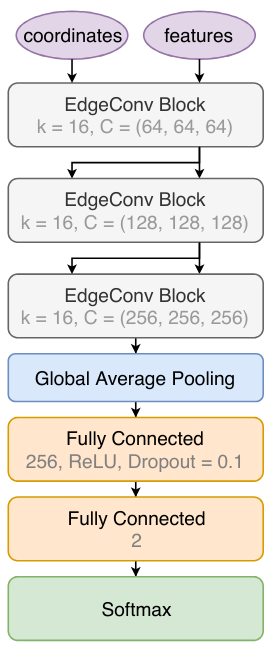
\includegraphics[scale =0.5]{ParticleNet.png}
        \caption{}
        \label{subfig:PNet_architecture}
    \end{subfigure}
    \begin{subfigure}{0.45\textwidth}
        \centering
        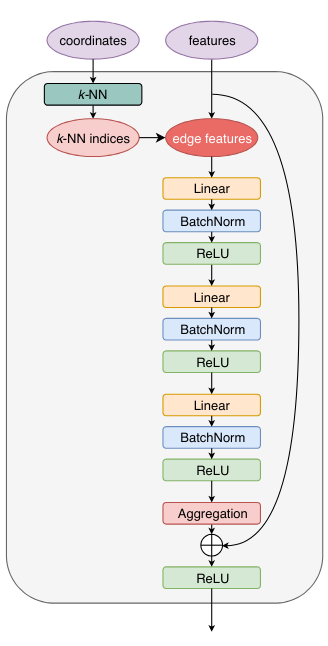
\includegraphics[scale =0.5]{ParticleNet2.png}
        \caption{}
        \label{subfig:PNet_block}
    \end{subfigure}
    
    \caption{(a) The architecture of the ParticleNet. (b) The structure of the EdgeConv block \cite{ParticleNet}}
    \label{fig:PNet}
\end{figure}
\indent The core concept of ParticleNet is the edge convolution operation, referred to as EdgeConv. The EdgeConv is a convolution-like operation for point clouds or in our case, particle clouds, which is realized by applying feature aggregation for each particle and its k nearest particles in the jet. ParticleNet's architecture consists of three EdgeConv blocks as illustrated in Figure \ref{subfig:PNet_architecture}. The specific process of each EdgeConv block is depicted in the Figure \ref{subfig:PNet_block}. It starts by finding the k-nearest neighbors for each particle within the jet. The edge between each particle and its k-nearest neighbors is determined using the input features of each particle. The EdgeConv operation is implemented as a three-layer multilayer perceptron (MLP). Each layer consists of a linear transformation, followed by a batch normalization and then a rectified linear unit (ReLU). Apart from the number of neighbors, an EdgeConv block is also characterized by the number of channels, $C =(C_1,C_2,C_3)$, corresponding to the number of units in each linear transformation layer. In the first EdgeConv block, the spatial coordinates ($\Delta\eta$, $\Delta\phi$) of the particles in the pseudorapidity-azimuth space are used to compute the edge of each pair of particles, while the subsequent EdgeConv blocks use the learned feature vectors as coordinates. The input features, differ from one task to another but generally include kinematic variables constructed with the 4-momentum of each particle, the PID information, the charge, and some impact parameters.\\
\indent After the EdgeConv blocks, a channel-wise global average pooling operation is applied to aggregate the learned features over all particles in the cloud. This is followed by a fully connected layer with 256 units and the ReLU activation. A dropout layer with a drop probability of 0.1 is included to prevent overfitting. A fully connected layer with two units, followed by a softmax function\footnote{The softmax function converts a vector of $K$ real numbers into a probability distribution of K possible outcomes. The softmax function is often used as the last activation function of a neural network to normalize the output of a network to a probability distribution over predicted output classes.}, is used to generate the output for the classification task. We then use this output, which is in the form of scores, corresponding to the cases listed in Table \ref{tab:classes}.
\begin{table}[H]
    \caption{Classes definition for jet tagging}
    \label{tab:classes}
	\centering\small
	\begin{tabular}{lll}\hline
		class & jets, at generator level, \dots & Definition\\ \hline
		bb & with two or more b hadrons & \(\mathrm{nBHadrons} > 1\)\\
		 b  & with exactly one b hadron & \(\mathrm{nBHadrons} =  1\)\\
		cc&  with two or more c, but no b hadrons& \(\mathrm{nBHadrons} = 0 \And 
		\mathrm{nCHadrons} > 1\) \\
		c & with exactly one c, but no b hadrons & \(\mathrm{nBHadrons} = 0 \And
		\mathrm{nCHadrons} = 1\)\\
		uds & induced by  u,  d, or s partons & \(\mathrm{hadronflavor} = 0 \And \left|\text{partonflavor}\right| \in \{1, 2, 3\}\)\\
		g & induced by g partons & \(\mathrm{hadronflavor} = 0 \And \mathrm{partonflavor} = 21\)
	\end{tabular}
\end{table}

From this, we establish two discriminating scores. One differentiates between heavy flavor (HF) jets  (type bb, b, cc or c) and light flavor (LF) jets (type uds or type g):
\[\mathrm{score}[\text{HF vs. LF}] =  \frac{\mathrm{score}[\text{bb}] + \mathrm{score}[\text{b}] + \mathrm{score}[\text{cc}] + \mathrm{score}[\text{c}]}{\mathrm{score}[\text{bb}] + \mathrm{score}[\text{b}] + \mathrm{score}[\text{cc}] + \mathrm{score}[\text{c}] + \mathrm{score}[\text{uds}] + \mathrm{score}[\text{g}]}\]
The second differentiates between charm and bottom induced jets
\[\mathrm{score}[\text{b vs. c}]  = \frac{\mathrm{score}[\text{bb}] + \mathrm{score}[\text{b}]}{ \mathrm{score}[\text{cc}] + \mathrm{score}[\text{c}] + \mathrm{score}[\text{bb}] + \mathrm{score}[\text{b}]}\]
Instead of using the entire score output in our analysis, we divide the two-dimensional plane defined by these two scores into categories enriched in  either LF, c, or b jets. These categories are illustrated in Figure \ref{fig:object:taggingcategories}. Each category is labeled with a letter L, C, or B, representing the dominant flavor (LF, c, or b jets) in that category. The subsequent index increases with higher purity of the corresponding flavor. Additionally, we define a loose, medium, and tight working point, starting at index 0, 1, and 2, respectively.
\begin{figure}[H]
	\centering
	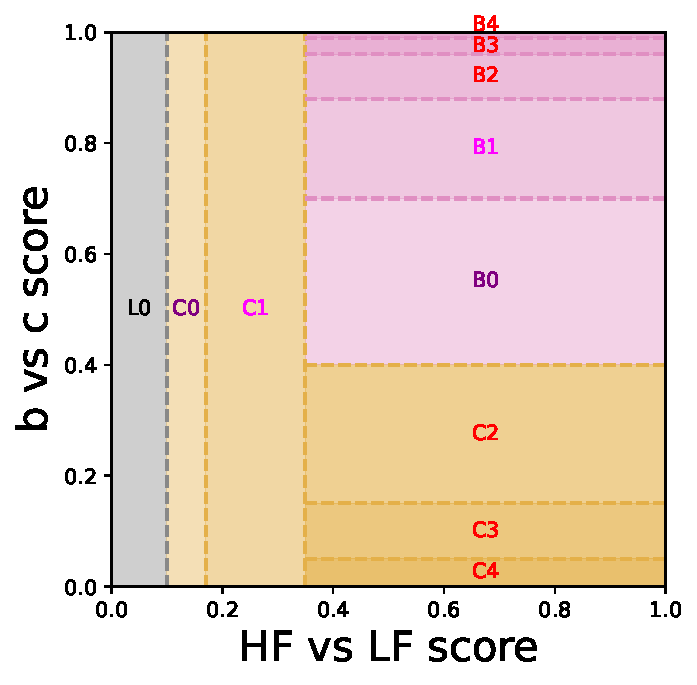
\includegraphics[width=\linewidth, height=0.33\textheight, keepaspectratio]{tagging_categories.pdf}
	\caption{Jet tagging categories used in the analysis. The C and B categories with indices 2 or higher are considered tightly tagged (red), one or higher medium (magenta + red), zero and higher loose (purple + magenta + red).}
	\label{fig:object:taggingcategories}
\end{figure}

\subsection{\label{subsec:ParT}Event classification with Particle Transformer}
\noindent Like ParticleNet, Particle Transformer is a Deep Neural Network (DNN) designed to be invariant under permutations of its input particles. However, there are two main differences between them. First, as its name suggests, Particle Transformer is based on a transformer architecture, whereas ParticleNet, discussed in the previous section, employs a convolutional architecture. Second, while ParticleNet does not explicitly focus on pairwise interactions between particles, Particle Transformer does, and is therefore more sensitive to correlations between them.\\
\indent An overview of the Particle Transformer's architecture is presented in Figure \ref{subfig:ParT_1}. As a Transformer architecture, its fundamental layer is called Attention. In our case, it is specifically the Particle Attention Block, which is illustrated in Figure \ref{subfig:ParT_2}. It consists of two stages. The first stage features a multi-head attention (MHA) module, with a LayerNorm (LN) layer both preceding and following it. The second stage includes a 2-layer MLP, with an LN before each linear layer and a Gaussian Error Linear Unit (GELU)\footnote{The Gaussian Error Linear Unit (GELU) is a neural network activation function that provides a smoother alternative to ReLU.} nonlinearity in between. A stack of $L$ of these particle attention blocks is employed. Following this, two class attention blocks and a global class token $x_{\text{class}}$ are utilized. The class attention block, depicted in Figure \ref{subfig:ParT_3}, has a similar structure as the particle attention block. In this block, the attention between $x_{\text{class}}$ and all the particles is computed using the standard MHA. The class token is then passed through a single-layer MLP, followed by a softmax function, to generate the final classification scores.












\begin{figure}[H]
    \centering
    \begin{subfigure}{1.0\textwidth}
        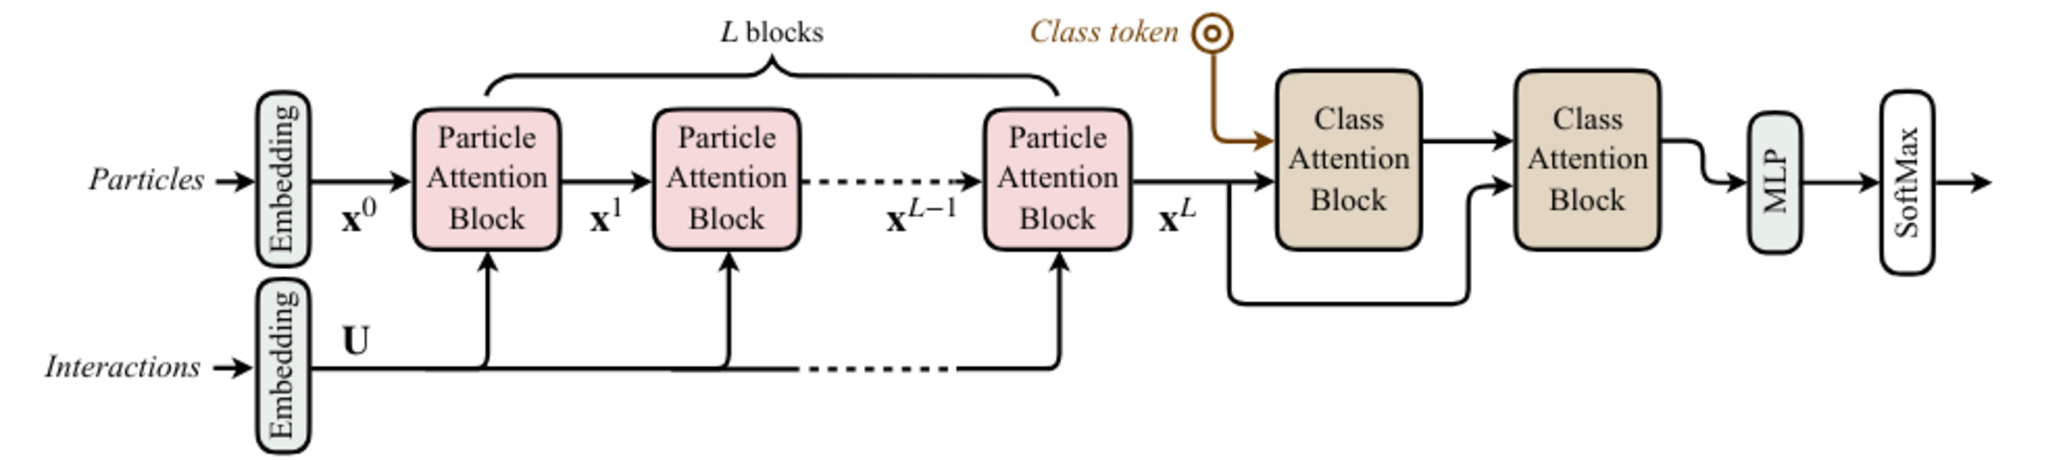
\includegraphics[width=1.0\linewidth]{ParT.pdf}
        \caption{}
        \label{subfig:ParT_1}
    \end{subfigure}

    \vspace{0.1cm}
    
    \begin{subfigure}{0.63\textwidth}
    \centering
        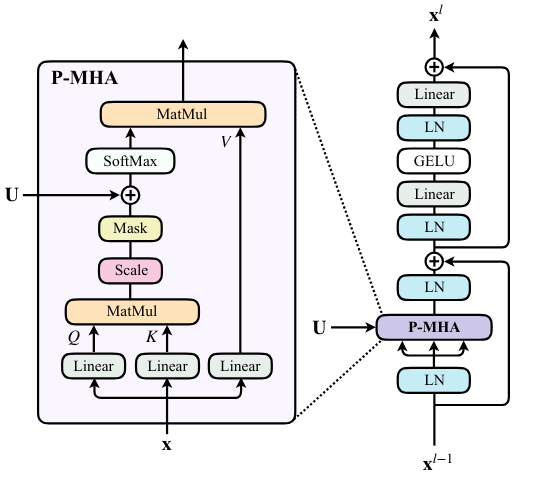
\includegraphics[scale=0.5]{ParT_2.png}
        \caption{}
        \label{subfig:ParT_2}        
    \end{subfigure} 
    \begin{subfigure}{0.33\textwidth}
    \centering
        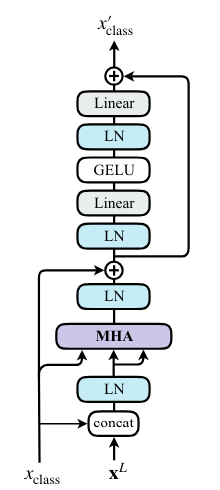
\includegraphics[scale=0.5]{ParT_3.png}
        \caption{}
        \label{subfig:ParT_3}        
    \end{subfigure} 
    \caption{The architecture of (a) Particle Transformer (b) Particle Attention Block (c) Class Attention Block \cite{ParticleTransformer}}
    \label{fig:ParT}
\end{figure}

The Particle Transformer model takes $\ln{p_T}$, $\ln{E}$, $\eta$, and $\phi$ for each lepton and jet, as well as $\ln{E_\text{MET}}$. Additionally, each lepton is given an "isEl/isMu" flag to enable the Particle Transformer to differentiate between the electron and muon streams more effectively. For each event used during training, all highest $p_T$ jets are used up to a channel dependent maximum: 10 for full-hadronic, 8 for single leptonic, and finally 6 for the dilepton channel. Each jet is paired with eight flags indicating which ParticleNet b- and c-tagging score thresholds the jet passes. Events in the training sample are weighted by cross-section, then renormalized such that the sum of the weights in each category is the same.

In the single-lepton and dilepton channels, a total of ten event categories are used during the training, one for each of the following processes:  The five t$\bar{\text{t}}$ backgrounds t$\overline{\text{t}}$+bb, t$\overline{\text{t}}$+bj, t$\overline{\text{t}}$+cc, t$\overline{\text{t}}$+cj and t$\overline{\text{t}}$+lf; the three Z backgrounds t$\bar{\text{t}}$Z(Z$\rightarrow\text{c}\bar{\text{c}}$), t$\bar{\text{t}}$Z(Z$\rightarrow\text{b}\bar{\text{b}}$), and t$\bar{\text{t}}$Z(Z$\rightarrow\text{q}\bar{\text{q}}$); the t$\bar{\text{t}}$H(H$\rightarrow\text{b}\bar{\text{b}}$) background and finally the t$\bar{\text{t}}$H(H$\rightarrow\text{c}\bar{\text{c}}$) signal process. The trained model assigns ten scores that reflect the probability of an event falling into each category, but since the scores must sum to 1, the result is nine independent Particle Transformer scores. The fully hadronic channel uses the same set-up, but adds an additional category for QCD events, bringing the total event category up to eleven and the number of independent scores to 10. The natural next step is to categorize all events based on their Particle Transformer scores by sorting each event into the category corresponding to its largest score. A cut of $(ttH_{cc}+ttH_{bb}+ttZ_{bb}+ttZ_{cc})/(1-ttZ_{qq}) > 0.85$ in these scores, defines the search region of our analysis. In Figure \ref{fig:signalex:FH:SR} an example of the Particle Transformer's output is presented for the t$\bar{\text{t}}$Z and t$\bar{\text{t}}$H categories in case of the FH channel, while the corresponding output for the t$\bar{\text{t}}$+jets categories is shown in Figure \ref{fig:signalex:FH:CR}.
 \begin{figure}[H]
    \centering
\foreach \n in {6,...,9}{
\includegraphics[width=0.41\linewidth, page=\n]{search_region_blinded.pdf}%
}
    \caption{Renormalized scores in the search region with all years combined for the t$\overline{\text{t}}$H categories (top) and the t$\overline{\text{t}}$Z categories (bottom) in the FH channel. Data points are not included because the analysis is blinded.}
    \label{fig:signalex:FH:SR}
\end{figure}

\begin{figure}[H]
    \centering
\foreach \n in {1,...,5}{
\includegraphics[width=0.43\linewidth, page=\n]{search_region_blinded.pdf}%
}
    \caption{Renormalized scores in the search region with all years combined for t$\bar{\text{t}}$+jets categories in the FH channel. Data points are not included because the analysis is blinded.}
    \label{fig:signalex:FH:CR}
\end{figure}

\section{\label{se:analysis_tt+bb}t$\overline{\text{t}}$+b$\overline{\text{b}}$ simulation}
\noindent Many measurements performed at pp collider experiments rely on accurate simulation to estimate background processes with similar signatures in the detectors compared to the process of interest (signal process). In such measurements, a subset of events is selected that contain a large fraction of events stemming from the signal process. In order to determine the contribution of the signal process to a set of selected events, an estimation of known SM-like processes can be performed via simulation of the known processes. As we saw in the previous section, the main background process, in our case, is t$\overline{\text{t}}$+b$\overline{\text{b}}$. Therefore better understanding of the t$\overline{\text{t}}$+b$\overline{\text{b}}$ process is important, as an accurate and reliable description of the t$\overline{\text{t}}$+b$\overline{\text{b}}$ process will allow for a measurement of our signal process with higher accuracy.\\
\indent A detailed study of the t$\overline{\text{t}}$+b$\overline{\text{b}}$ process is also of interest due to the challenging modeling of the process. In summary, the t$\overline{\text{t}}$+b$\overline{\text{b}}$ process is difficult to model accurately as it contains b quarks with low but non-negligible masses, and, by comparison, heavy top quarks. Hence, finding appropriate energy scales for the calculation of t$\overline{\text{t}}$+b$\overline{\text{b}}$ MEs and interfacing the MEs with PS and PDF calculations is a difficulty. Uncertainties related to the choice of renormalization and factorization scales can, in ME calculations at NLO in QCD, lead to uncertainties of up to 50\% in fiducial and differential cross section predictions of t$\overline{\text{t}}$+b$\overline{\text{b}}$ \cite{Tom}. Improved knowledge in this process via fiducial and differential measurements of t$\overline{\text{t}}$+b$\overline{\text{b}}$ is therefore of prime interest in order to validate or discard scale choices made for state-of-the-art simulations.

\subsection{\label{motivation}Motivation}


% One goal of the t$\overline{\text{t}}$+b$\overline{\text{b}}$ measurement in this
% thesis is to gain improved understanding of this important and irreducible background
% process for the two aforementioned measurements and thereby improve the sensitivity
% of the measurements of these processes.

% A detailed study of the t$\overline{\text{t}}$+b$\overline{\text{b}}$ process is also of interest due to the challenging modeling of
% the process. . In summary, the t$\overline{\text{t}}$+b$\overline{\text{b}}$ process is difficult to model accurately as it contains b quarks with low but non-negligible
% masses, and, by comparison, heavy top quarks. Hence, finding appropriate energy scales
% for the calculation of t$\overline{\text{t}}$+b$\overline{\text{b}}$ MEs and interfacing the MEs with PS and pdf calculations is a
% difficulty. Uncertainties related to the choice of renormalization and factorization scales
% can, in ME calculations at NLO in QCD, lead to uncertainties of up to 50\% in fiducial and
% differential cross section predictions of t$\overline{\text{t}}$+b$\overline{\text{b}}$ [137]. Improved knowledge in this process
% via fiducial and differential measurements of t$\overline{\text{t}}$+b$\overline{\text{b}}$ is therefore of prime interest in order
% to validate or discard scale choices made for state-of-the-art simulations. A more accurate
% modeling of the process can then improve the central prediction in the modeling of this
% background process, e.g. in the measurements of the ttH(bb) and tt tt processes, and give
% a better estimate of the uncertainties associated with the modeling of the t$\overline{\text{t}}$+b$\overline{\text{b}}$ process

% The measurements presented in this thesis aim at verifying the t$\overline{\text{t}}$+b$\overline{\text{b}}$ simulation models
% and how these describe the process as a function of selected observables. This measurement consists of fiducial cross section measurements and normalized differential cross
% section measurements. A set of fiducial phase space regions and observables has been
% chosen to be measured and will be detailed in Section 8.2. Previous measurements by the
% ATLAS and CMS Collaborations showed that the cross section of t$\overline{\text{t}}$+b$\overline{\text{b}}$ is under-predicted
% by all simulation approaches tested in these measurements. Differential distributions
% probed in these measurements generally show good agreement but are measured with
% large uncertainties which do not allow for ruling out any of the tested simulation approaches and their modeling choices (such as the renormalization or factorization scales)
\begin{figure}[H]
    \centering
    \begin{subfigure}{0.49\textwidth}
        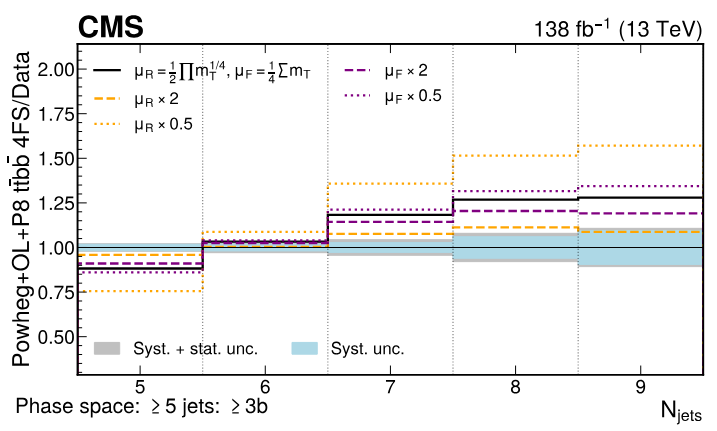
\includegraphics[width=1.0\linewidth]{TOP_1.png}
        \caption{}
    \end{subfigure}
    \begin{subfigure}{0.49\textwidth}
        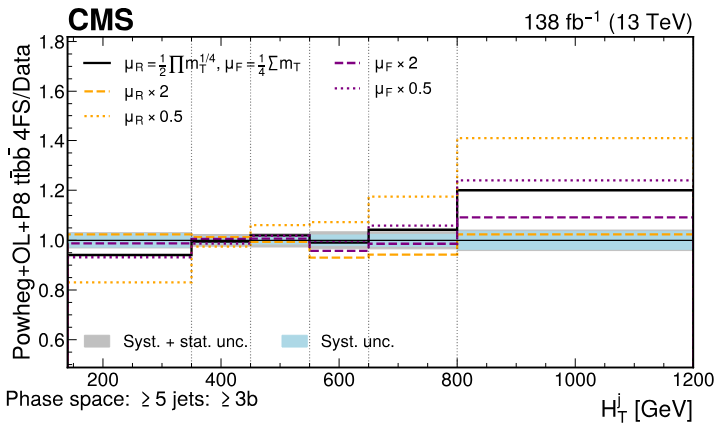
\includegraphics[width=1.0\linewidth]{TOP_2.png}
        \caption{}
    \end{subfigure}
    \caption{Ratio of normalized differential cross section predictions of the \textsc{Powheg}+OL+P8 t$\overline{\text{t}}$+b$\overline{\text{b}}$ \textsc{4fs} modeling approach with different $\mu_R$ and $\mu_F$ scale settings relative to the measured normalized differential cross sections for (a) the number of jets and (b) $H_T$ of jets in the $\geq$5 jets: $\geq$3b phase space \cite{TOP-22-009}}
    \label{fig:TOP-22-009_1}
\end{figure}
\noindent Previous analyses by the CMS Collaboration \cite{TOP-22-009} studied some variations of the t$\overline{\text{t}}$+b$\overline{\text{b}}$ $\mu_R$ and $\mu_F$ scales in order to check their compatibility with the data compared to the nominal model. The results are shown in Figures \ref{fig:TOP-22-009_1}, \ref{fig:TOP-22-009_2}. For these results, the t$\overline{\text{t}}$+b$\overline{\text{b}}$ matrix element was calculated using {\fontfamily{bch}\fontshape{sc}\selectfont{Powheg}} and {\fontfamily{bch}\fontshape{sc}\selectfont{OpenLoops}} (OL) at NLO in QCD, utilizing the four-flavor-scheme ({\fontfamily{bch}\fontshape{sc}\selectfont{4fs}}), where b quarks are not part of the proton PDF, and matched with {\fontfamily{bch}\fontshape{sc}\selectfont{Pythia}}-8 (P8) for parton showering and hadronization. From these results, it is clear that the $\mu_R\times2$ and $\mu_F\times2$ variations improve the description. In addition, a measurement of the fiducial t$\overline{\text{t}}$+b$\overline{\text{b}}$ cross sections was performed \cite{vanderLinden}. In this study, as it is illustrated in \ref{fig:vanderLinden}, we can see that $\mu_R\times2$ and $\mu_F\times2$ variations decrease the fiducial cross section predictions, with $\mu_R\times2$ decreasing too much, beyond what we measure in data, while $\mu_F\times2$ is compatible. Motivated by these results, our study in this thesis, focuses mainly on the $\mu_F\times2$ variation, compared with the nominal, within the context of our t$\overline{\text{t}}$H analysis.
\begin{figure}[H]
    \centering
    \begin{subfigure}{0.49\textwidth}
        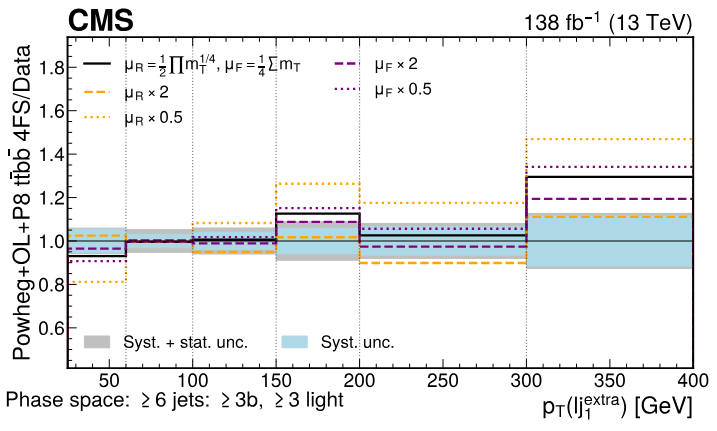
\includegraphics[width=1.0\linewidth]{TOP_3.png}
    \end{subfigure}
    \begin{subfigure}{0.49\textwidth}
        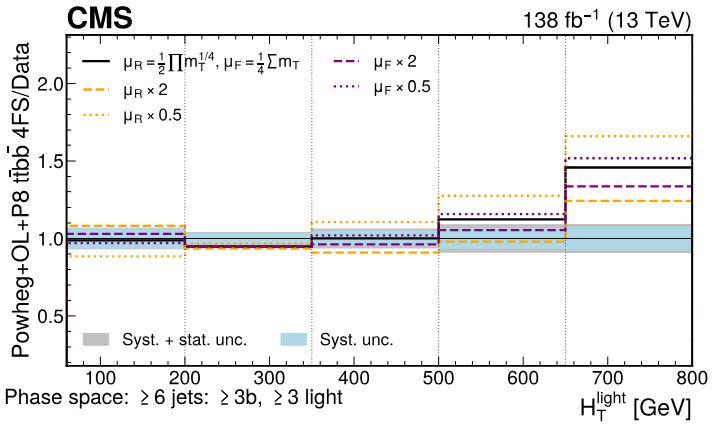
\includegraphics[width=1.0\linewidth]{TOP_4.png}
    \end{subfigure}
    \caption{Ratio of normalized differential cross section predictions of the \textsc{Powheg}+OL+P8 t$\overline{\text{t}}$+b$\overline{\text{b}}$ \textsc{4fs} modeling approach with different $\mu_R$ and $\mu_F$ scale settings relative to the measured normalized differential cross sections for (a) the extra light jet and (b) $H_T$ of light jets in the $\geq$6 jets: $\geq$3b, $\geq$3 light phase space \cite{TOP-22-009}}
    \label{fig:TOP-22-009_2}
\end{figure}
\begin{figure}[H]
    \centering
    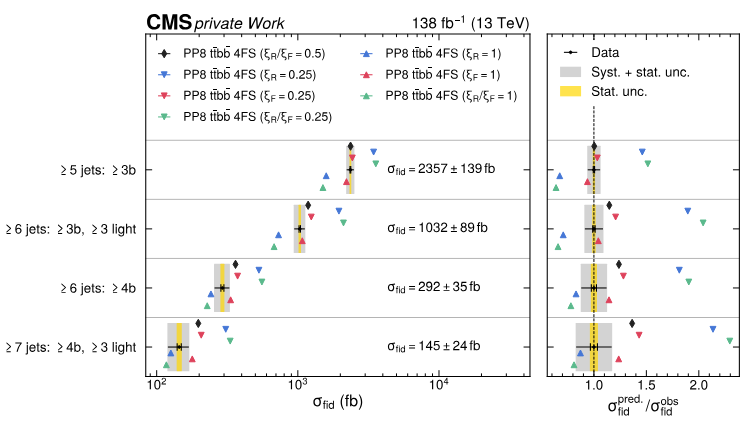
\includegraphics[width=0.6\linewidth]{Jan.png}
    \caption{Fiducial cross sections measurement compared to the \textsc{Powheg}+OL+P8 \textsc{4fs} signal model and alternative $\mu_R$ and $\mu_F$ scale choices. Variations of the $\mu_R$ and $\mu_F$ scales by factors of two up and down are indicated via triangles. The nominal values for $\mu_F$ and $\mu_R$ correspond to $\xi_F = 0.5$, $\xi_R =0.5$ respectively \cite{vanderLinden}.}
    \label{fig:vanderLinden}
\end{figure}

% One thing to note is that this does not remove the trend to predict higher cross sections in more exclusive phase spaces (mostly dominated by the 3b vs 4b fraction mismodeling), so just changing µF is not a solution for everything, but overall improves the picture a bit

\subsection{\label{generator}Generator configuration}
\noindent {\fontfamily{bch}\fontshape{sc}\selectfont{Powheg Box Res}} \cite{Jezo:2015aia} is the main tool used for event simulation of t$\overline{\text{t}}$+b$\overline{\text{b}}$ events in the scope of this thesis. The generator uses the {\fontfamily{bch}\fontshape{sc}\selectfont{Powheg}} method for interfacing PS generators with NLO QCD computations as described in Section \ref{subsec:POWHEG}. {\fontfamily{bch}\fontshape{sc}\selectfont{Powheg Box Res}} requires an input file, in which different variables, dependent on the process, are defined. An example of an input file for the t$\overline{\text{t}}$+b$\overline{\text{b}}$ package can be found in the Appendix \ref{chap:apx_exp_data}. The output of the generator is a Les Houches Event (LHE) File \cite{LHE}, containing the input file as a header, followed by the initialization and state of the Random Number Generator (RNG) and the event data. The information is wrapped in XML\footnote{XML stands for Extensible Markup Language} structure \cite{XML}.\\
\indent {\fontfamily{bch}\fontshape{sc}\selectfont{Powheg Box Res}} generates events through a linear process consisting of four stages. These stages can be executed on a single core or parallelized across multiple cores, which is particularly useful for simulating complex processes or at next-to-leading order (NLO). In this thesis, only the parallelized mode is considered. The main advantage of parallelization in {\fontfamily{bch}\fontshape{sc}\selectfont{Powheg Box Res}} is to increase statistical accuracy rather than reduce runtime. This means that the total computational effort is not distributed across multiple parallel runs but is the result of multiplying the computations of a single run by the number of parallel runs. Each parallel run uses a different random seed, ensuring statistical independence, and their results can be combined.\\ 
\indent In parallel execution mode, the next stage starts only after all parallel computations for the current stage are completed. The output from these computations is written in a file and combined at the beginning of the next stage, ensuring all parallel runs start with the same data. As the necessary information is stored after each stage, the simulation can be resumed at any point.\\
\indent The four stages of computations in a {\fontfamily{bch}\fontshape{sc}\selectfont{Powheg Box Res}} simulation are the following:
\begin{enumerate}
    \item \textbf{Importance sampling grids}. As discussed in Section \ref{sec:MC_method}, MC integration can be improved by importance sampling. {\fontfamily{bch}\fontshape{sc}\selectfont{Powheg Box Res}} implements this method by generating points in a d-dimensional ([0, 1]$\times$[0, 1])-plane, mapped to the actual integral that needs to be estimated. These points constitute the importance sampling grids, in the following simply referred to as sampling grids. The shape of the sampling grids represents their quality. It can be examined in visualizations accessible through a .top\footnote{The name extension .top, indicates that the file format is appropriate for the portable \textsc{Top Drawer} graphics package} file which is only created when the parallel executed computations have been combined either in a next iteration of the first stage or by execution of the second stage. If the shape of the visualized sampling grid is not smooth, this hints at insufficient statistics which then leads to unusable samples as the integral kernel cannot be accurately estimated. {\fontfamily{bch}\fontshape{sc}\selectfont{Powheg Box Res}} provides options to increase the number of sampled phase space points. This can be done directly by increasing the number of parallel runs, by running the first stage multiple times, or by a combination of both. Each iteration of the first stage is treated as a distinct stage, meaning all parallel computations of one iteration must be completed before the next iteration can begin, with results from the previous iteration combined.
    \item \textbf{Cross section computations}. Once the previously constructed sampling grids are combined and the associated .top file is created, a multidimensional step function is calculated and stored on the sampling grid. This function acts as an upper bound on the integrand, aiding in the integral estimation. The number of calls for these computations can be directly set and increased by either running more parallel executions or performing multiple iterations of this stage.
    \item \textbf{Generation of radiation}. In addition to combining the stage 2 computations, additional files are generated, containing all the information from the previous two stages. A human-readable text file with details on the cross section is also created. Subsequently, the upper bounding factors for radiation generation are calculated. These factors are used for simulating the hardest emission at NLO, following the {\fontfamily{bch}\fontshape{sc}\selectfont{Powheg}} method. While the number of calls to the relevant functions can be configured by the user, this stage cannot be repeated for multiple iterations.
    \item \textbf{Event generation}. At this stage, the program loads the previously generated files to produce events, which are then saved in an LHE file. The user determines the number of events, and this number can be increased later by re-executing this stage with new seeds.
\end{enumerate}

\subsubsection{Input parameters}
\noindent As it was mentioned in the previous section, {\fontfamily{bch}\fontshape{sc}\selectfont{Powheg Box Res}} requires an input file, with different variables. Here we present some of the most important ones. First, heavy-quark mass effects are included throughout using 
 \begin{equation}
     m_t = 172.5 \: \text{GeV} \:\:\:\:\: \text{and} \:\:\:\:\:  m_b = 4.75 \: \text{GeV}
 \end{equation}
All other quarks are treated as massless in the perturbative part of the calculations. Since we use massive b-quarks, for the PDF evolution and the running of $\alpha_s$ we adopt the four-flavor-scheme ({\fontfamily{bch}\fontshape{sc}\selectfont{4fs}}). Thus, for consistency, we renormalise $\alpha_s$ in the decoupling scheme, where top- and bottom-quark loops are subtracted at zero momentum transfer. In this way, heavyquark loop contributions to the evolution of the strong coupling are effectively described at first order in $\alpha_s$ through the virtual corrections. \\
\indent For the calculation of hard cross sections at NLO, as well as for the generation of the first {\fontfamily{bch}\fontshape{sc}\selectfont{Powheg}} emission, we use the NNPDF31\_nnlo\_as\_0118\_nf\_4 parton distributions \cite{NNPDF} as implemented in the LHAPDFs \cite{LHAPDF} and the corresponding $\alpha_s^{(4F)}$.
 
\subsubsection{Scale choices}
\noindent Because of its strong interaction origin, the t$\overline{\text{t}}$+b$\overline{\text{b}}$ cross section scales with $a_s^4$, and is therefore highly sensitive to the choice of renormalization scale $\mu_R$ (see Section \ref{subsec:PDF}). As the t$\overline{\text{t}}$+b$\overline{\text{b}}$ process incorporates a top quark and a b quark, in Ref. \cite{Tom} choices of the renormalization scale for an ME-level simulation are recommended as
\begin{equation}
    \mu_R = \frac{1}{2}\sqrt{\mu_{t\overline{t}}\mu_{b\overline{b}}}
\end{equation}
where $\mu_{t\overline{t}}$ and $\mu_{b\overline{b}}$ are defined as the geometric average of the transverse masses of the t$\overline{\text{t}}$ and b$\overline{\text{b}}$ systems,
\begin{equation}
    \mu_{t\overline{t}} = \sqrt{m_T(t)m_T(\overline{t})} \:\:\:\:\:\: \text{and} \:\:\:\:\:\:  \mu_{b\overline{b}} = \sqrt{m_T(b)m_T(\overline{b})}
\end{equation}
resulting in 
\begin{equation}
    \mu_R = \frac{1}{2}\big[m_T(t) \cdot m_T(\overline{t}) \cdot m_T(b) \cdot m_T(\overline{b})\big]^{1/4}
\end{equation}
Here, the transverse mass is defined as $m_T(i) = \sqrt{m^2(i) +p_{T}^2(i)}$. For the factorization scale $\mu_F$, recommended choice is
\begin{equation}
    \mu_F = \frac{1}{4}\big[m_T(t) + m_T(\overline{t}) + m_T(b) + m_T(\overline{b}) + m_T(g)\big]
\end{equation}

\subsubsection{Damping parameter}
\noindent As we saw in Section \ref{subsec:POWHEG}, the master formula for the description of NLO radiation in the {\fontfamily{bch}\fontshape{sc}\selectfont{Powheg}} approach consists of two contributions which arise from the splitting of real emission into singular (S) and finite (F) parts as described by Equation (\ref{eq:Real_cross}). For the splitting of these two parts, we introduced a parameter $h$, or as it is usually called, $h_{damp}$. This freely adjustable parameter in {\fontfamily{bch}\fontshape{sc}\selectfont{Powheg}} represents the matching scale between the ME calculation and the PS. Basically, $h_{damp}$ describes the damping of radiation with a high transverse momentum. It separates the low and the high transverse momentum regions and controls the hardest radiation. \\
\indent In the context of the t$\overline{\text{t}}$+b$\overline{\text{b}}$ simulation, we define this parameter as,
\begin{equation}
    h_{damp} = \sqrt{\frac{1}{2}}\big(m_T(t) + m_T(\overline{t})\big)\cdot \text{dynhdampPF}
\end{equation}
Therefore, any variation in this damping parameter is introduced through the dynhdampPF variable. The nominal value of this variable is set to dynhdampPF  $= 0.5$. For our study we introduce two variations which we will refer to as \textit{hdampUP} and \textit{hdampDOWN} where the dynhdampPF variable is set to $0.835$ and $0.317$ respectively. In Table \ref{tab:number of events} the number of events generated for each one of these variations across the three channels is presented. Specifically, the total number of events generated for the purpose of this thesis is 205 million, since we generate the events presented in Table \ref{tab:number of events} for both $\mu F\times$1 and $\mu F\times$2. The distribution of the events, of course, is not random but mirrors the number of events of the Run 2 samples used in the t$\overline{\text{t}}$H analysis.

\begin{table}[H]
\centering
\caption{Number of events generated for each damping parameter across the three channels}
\label{tab:number of events}
\begin{tabular}{l|ccc}
                   & DL   & SL   & FH   \\ \hline
dynhdampPF = 0.5   & 12 M & 25 M & 19 M \\
dynhdampPF = 0.835 & 8 M  & 10 M & 7 M  \\
dynhdampPF = 0.317 & 7 M  & 10 M & 7 M 
\end{tabular}
\end{table}
\subsection{Observables}
\noindent To investigate the effect of different parameter choices, one needs to perform tests on observables which are sensitive to these parameters. For this MC generator study, all three channels are analyzed. Depending on the channel we have different number of jets in the final state according to the W boson decays. For all channels, we have four b/$\overline{\text{b}}$ quarks, two from the initial process which will refer to as \textit{prompt} and two from the t/$\overline{\text{t}}$ decay.\\
\indent The renormalization scale, factorization scale and the h$_{damp}$ are parameters affecting the kinematics of the hadrons in the system. Observables related to hadron momentum or momentum of a system consisting of two hadrons are sensitive to these parameters. The observables studied are shown in the Table \ref{tab:observables}. In the following sections, only a few selected observables will be presented, while the rest of them can be found in Appendix \ref{chap:apx_B}.
\subsection{\label{DL}Dileptonic channel}
\noindent As it was discussed in Chapter \ref{chap:first}, the dileptonic (DL) channel involves four leptons in the final state, two charged and two neutral, originating from the two W boson decays. It is the easiest channel to model amongst the others due to the lower number of jets. The only jets that appear in the final state are from the four b/$\overline{\text{b}}$ quarks, as it was mentioned in the previous section, as well as the extra emission that is generated for the NLO calculation.\\
\newpage
\clearpage
   \newgeometry{left=0.5cm, right=0.5cm, top=0.5cm, bottom=0.5cm} % new margins
   \thispagestyle{empty}
\begin{table}[ht]
\centering
\small
\caption{Description of all measured observables for each of the three channels}
\label{tab:observables}
\begin{tabular}{lllll}
                              & \multicolumn{1}{c}{Observable}                                            & \multicolumn{1}{c}{DL} & \multicolumn{1}{c}{SL} & \multicolumn{1}{c}{FH} \\ \hline
\multicolumn{5}{l}{Global observables} \\ \hline
$m(t\bar{t}+b\bar{b})$                 & Invariant mass of t$\overline{\text{t}}+$b$\overline{\text{b}}$ system                           & \checkmark             & \checkmark             & \checkmark             \\
$H_T(t\bar{t}+b\bar{b})$                 & Scalar sum of transverse momentum of t$\overline{\text{t}}+$b$\overline{\text{b}}$ system                           & \checkmark             & \checkmark             & \checkmark             \\
\multicolumn{5}{l}{Observables related to top quarks}                                                                                                                                \\ \hline
$E(t,\bar{t})$                & Energy of t/$\overline{\text{t}}$ quarks                                              & \checkmark             & \checkmark             & \checkmark             \\
$p_T(t,\bar{t})$              & Transverse momentum of t/$\overline{\text{t}}$ quarks                                 & \checkmark             & \checkmark             & \checkmark             \\
$m^{reco}(t, \bar{t})$        & Reconstructed mass of t/$\overline{\text{t}}$ quarks                                  & \checkmark             & \checkmark             & \checkmark             \\
$y(t,\bar{t})$                & Rapidity of t/$\overline{\text{t}}$ quarks                                            & \checkmark             & \checkmark             & \checkmark             \\
$\phi(t,\bar{t})$             & Azimuthial angle of t/$\overline{\text{t}}$ quarks                                    & \checkmark             & \checkmark             & \checkmark             \\
$\Delta R(t\bar{t})$          & Angular separation of t$\overline{\text{t}}$ system                       & \checkmark             & \checkmark             & \checkmark             \\
$H_T(t\bar{t})$               & Scalar sum of transverse momentum of t$\overline{\text{t}}$ system        & \checkmark             & \checkmark             & \checkmark             \\
$m(t\bar{t})$                 & Invariant mass of t$\overline{\text{t}}$ system                           & \checkmark             & \checkmark             & \checkmark             \\
$y(t\bar{t})$                 & Rapidity of t$\overline{\text{t}}$ system                                 & \checkmark             & \checkmark             & \checkmark             \\
$p_T(t\bar{t})$                 & Transverse momentum of t$\overline{\text{t}}$ system                                 & \checkmark             & \checkmark             & \checkmark             \\
\multicolumn{5}{l}{Observables considering all pairs of b jets}                                                                                                                      \\ \hline
$E(b,\bar{b}^{all})$          & Energy of b/$\overline{\text{b}}$ quarks                                  & \checkmark             & \checkmark             & \checkmark             \\
$p_T(b,\bar{b}^{all})$        & Transverse momentum of b/$\overline{\text{b}}$ quarks                     & \checkmark             & \checkmark             & \checkmark             \\
$\eta(b,\bar{b}^{all})$       & Pseudorapidity of b/$\overline{\text{b}}$ quarks                          & \checkmark             & \checkmark             & \checkmark             \\
$\phi(b,\bar{b}^{all})$       & Azimuthial angle of b/$\overline{\text{b}}$ quarks                        & \checkmark             & \checkmark             & \checkmark             \\
\multicolumn{5}{l}{Observables related to the pair of b jets from $t\overline{t}$ decay}                                                                                             \\ \hline
$\Delta R(b\bar{b})$          & Angular separation of b$\overline{\text{b}}$ system                       & \checkmark             & \checkmark             & \checkmark             \\
$H_T(b\bar{b})$               & Scalar sum of transverse momentum of b$\overline{\text{b}}$ system        & \checkmark             & \checkmark             & \checkmark             \\
$m(b\bar{b})$                 & Invariant mass of b$\overline{\text{b}}$ system                           & \checkmark             & \checkmark             & \checkmark             \\
$y(b\bar{b})$                 & Rapidity of b$\overline{\text{b}}$ system                                 & \checkmark             & \checkmark             & \checkmark             \\
$p_T(b\bar{b})$                 & Transverse momentum of b$\overline{\text{b}}$ system                                 & \checkmark             & \checkmark             & \checkmark             \\
\multicolumn{5}{l}{Observables related to the pair of b jets not from $t\overline{t}$ decay ($b^{\text{prompt}}$)}                                                                          \\ \hline
$\Delta R(b\bar{b}^{\text{prompt}})$ & Angular separation of prompt b$\overline{\text{b}}$ system                & \checkmark             & \checkmark             & \checkmark             \\
$H_T(b\bar{b}^{\text{prompt}})$      & Scalar sum of transverse momentum of prompt b$\overline{\text{b}}$ system & \checkmark             & \checkmark             & \checkmark             \\
$m(b\bar{b}^{\text{prompt}})$        & Invariant mass of prompt b$\overline{\text{b}}$ system                    & \checkmark             & \checkmark             & \checkmark             \\
$y(b\bar{b}^{\text{prompt}})$        & Rapidity of prompt b$\overline{\text{b}}$ system                          & \checkmark             & \checkmark             & \checkmark             \\
$p_T(b\bar{b}^{\text{prompt}})$        & Transverse momentum of prompt b$\overline{\text{b}}$ system                          & \checkmark             & \checkmark             & \checkmark             \\
\multicolumn{5}{l}{Observables related to light jets from W decay}                                                                                                                   \\ \hline
$E(q_{lf})$                   & Energy of lf-quarks                                            &                        & \checkmark             & \checkmark             \\
$p_T(q_{lf})$                 & Transverse momentum of lf-quarks                               &                        & \checkmark             & \checkmark             \\
$\eta(q_{lf})$                & Pseudorapidity of lf-quarks                                    &                        & \checkmark             & \checkmark             \\
$\phi(q_{lf})$                & Azimuthial angle of lf-quarks                                  &                        & \checkmark             & \checkmark             \\
$\Delta R(q' \bar{q})$        & Angular separation of lf-quarks system                         &                        & \checkmark             & \checkmark             \\
$H_T(q' \bar{q})$             & Scalar sum of transverse momentum of lf-quarks system          &                        & \checkmark             & \checkmark             \\
$m(q' \bar{q})$               & Invariant mass of lf-quarks system                             &                        & \checkmark             & \checkmark             \\
$\eta(q' \bar{q})$            & Pseudorapidity of lf-quarks system                             &                        & \checkmark             & \checkmark             \\
\multicolumn{5}{l}{Observables related to leptons from W decay}                                                                                                                      \\ \hline
$E(l,\nu_l)$                  & Energy of leptons (charged or neutral)                                    & \checkmark             & \checkmark             &                        \\
$p_T(l,\nu_l)$                & Transverse momentum of leptons (charged or neutral)                       & \checkmark             & \checkmark             &                        \\
$\eta(l,\nu_l)$               & Pseudorapidity of leptons (charged or neutral)                            & \checkmark             & \checkmark             &                        \\
$\phi(l,\nu_l)$               & Azimuthial angle of leptons (charged or neutral)                          & \checkmark             & \checkmark             &                        \\
$\Delta R(l^- l^+)$           & Angular separation of charged leptons system                              & \checkmark             &                        &                        \\
$H_T(l^- l^+)$                & Scalar sum of transverse momentum of charged leptons system               & \checkmark             &                        &                        \\
$m(l^- l^+)$                  & Invariant mass of charged leptons system                                  & \checkmark             &                        &                        \\
$\eta(l^- l^+)$               & Pseudorapidity of charge leptons system                                   & \checkmark             &                        &                        \\
\multicolumn{5}{l}{Observables related to extra light jets}                                                                                                                          \\ \hline
$E(l_j^{\text{extra}})$              & Energy of extra light jet                                                 & \checkmark             & \checkmark             & \checkmark             \\
$p_T(l_j^{\text{extra}})$            & Transverse momentum of extra light jet                                    & \checkmark             & \checkmark             & \checkmark             \\
$\eta(l_j^{\text{extra}})$           & Pseudorapidity of extra light jet                                         & \checkmark             & \checkmark             & \checkmark             \\
$\phi(l_j^{\text{extra}})$           & Azimuthial angle of extra light jet                                       & \checkmark             & \checkmark             & \checkmark            
\end{tabular}
\end{table}
\newpage
\clearpage
\restoregeometry % restore the original margins
% \afterpage{
%   \clearpage
%   \newgeometry{left=0.5cm, right=0.5cm, top=0.5cm, bottom=0.5cm} % new margins
%   \thispagestyle{empty}

%   \clearpage
%   \restoregeometry % restore the original margins
% }
\indent As  expected, the observables that were found to be most sensitive to the different parameters used in our simulation, are the ones related to the transverse momentum. Specifically, in Figure \ref{fig:pt_DL}, the distributions of the transverse momentum for the t/$\overline{\text{t}}$ (\ref{subfig:pt(t,tbar)_DL}) and the b/$\overline{\text{b}}$ (\ref{subfig:pt(b_all)_DL}) quarks are presented. It is easy to see from the ratio plots, that the most significant parameter change is the different factorization scale. As the transverse momentum increases, the ratio of the $\mu_F \times 1$ sample over the $\mu_F \times 2$ sample for the nominal damping parameter, also increases for both t/$\overline{\text{t}}$ and b/$\overline{\text{b}}$ quarks. This effect is stronger in the case of t/$\overline{\text{t}}$, reaching up to 10\% difference. On the low $p_T$ spectrum, in case of the t/$\overline{\text{t}}$ quarks, we can see a very small drop in the ratio plot, indicating again, that for $\mu_F \times 2$, the t/$\overline{\text{t}}$ quarks are simulated to be less energetic. \\
\indent As for the h$_{\text{damp}}$ variations, it is obvious, that they basically have no effect. The results for both hdampUP and hdampDOWN variations are identical to the nominal selection for both $\mu_F \times 1$ and $\mu_F \times 2$ samples.
\begin{figure}[H]
    \centering
    \begin{subfigure}{0.49\textwidth}
        \centering
        \includegraphics[width= 1.1\linewidth]{DL/ratio_ttbar_pt.pdf}
        \caption{}
        \label{subfig:pt(t,tbar)_DL}        
    \end{subfigure}
    \hfill
    \begin{subfigure}{0.49\linewidth}
        \centering
        \includegraphics[width= 1.1\textwidth]{DL/ratio_b_all_pt.pdf}
        \caption{}
        \label{subfig:pt(b_all)_DL}
    \end{subfigure}
    \caption{Distribution of the transverse momentum of (a) the t/$\overline{\text{t}}$ and (b) the b/$\overline{\text{b}}$ quarks for the six different settings used in the simulation. The lower panel shows the ratio of the nominal setting to the variations. The shaded bands represent statistical uncertainties. The last bins contain the overflow events.}
    \label{fig:pt_DL}
\end{figure}
\indent Of course, since the transverse momentum is very sensitive to the different factorization scale selection, as we saw from the previous plots, we expect similar results from the H$_{\text{T}}$ variable. In Figure \ref{fig:HT_DL}, the results for the different t$\overline{\text{t}}$ and b$\overline{\text{b}}$ systems are presented. Obviously, the b quarks have been separated into the two different categories, depending on the mother particles that originate from.\\
\indent As expected, in Fig. \ref{subfig:HT(ttbar)_DL}, one can see again the same trend as before for the H$_{\text{T}}$ of the t$\overline{\text{t}}$ system. As for the b$\overline{\text{b}}$ system originating from the top quarks, it is clear that they inherit the same behavior. This, however, is not the case for the prompt b$\overline{\text{b}}$ system (Fig. \ref{subfig:HT(bbbar_prompt)_DL}).\\
\begin{figure}[htb!]
    \centering
    \begin{subfigure}{0.49\textwidth}
        \centering
        \includegraphics[width= 1.1\linewidth]{DL/ratio_tt_system_HT.pdf}
        \caption{}
        \label{subfig:HT(ttbar)_DL}
    \end{subfigure}
    \hfill
    \begin{subfigure}{0.49\textwidth}
        \centering
        \includegraphics[width= 1.1\linewidth]{DL/ratio_prompt_bs_HT.pdf}
        \caption{}
        \label{subfig:HT(bbbar_prompt)_DL}
    \end{subfigure}
    \hfill
    \begin{subfigure}{0.49\textwidth}
        \centering
        \includegraphics[width= 1.1\linewidth]{DL/ratio_bs_from_top_HT.pdf}
        \caption{}
        \label{subfig:HT(bbbar)_DL}
    \end{subfigure}
    \caption{Distribution of H$_{\text{T}}$ for (a) t$\overline{\text{t}}$, (b) prompt b$\overline{\text{b}}$ and (c) b$\overline{\text{b}}$, originating from top quarks, systems for the six different settings used in the simulation. The lower panel shows the ratio of the nominal setting to the variations. The shaded bands represent statistical uncertainties. The last bins contain the overflow events.}
    \label{fig:HT_DL}
\end{figure}
\indent The prompt b quarks, are generated from the initial particles alongside the top quarks. Therefore, due to the larger mass, the top quarks are more boosted, resulting in significant less energy and transverse momentum for the remaining b quarks. Since the different settings affect the higher values of p$_{\text{T}}$ and H$_{\text{T}}$, it is normal to not see any change for the different settings.\\ 
\indent This difference in the features of the two systems can be seen in Figure \ref{fig:dR_DL}, where the angular separation is presented. More specifically, as we can see from Fig. \ref{subfig:dR(ttbar)_DL}, there is a peak in the distribution of the angular separation of the t$\overline{\text{t}}$ system which represents that the two top quarks are predominally produced centrally ($\Delta\eta \sim 0$) and back-to-back ($\Delta\phi \sim \pi$). This of course happens, due to the fact that, the two top quarks carry most of the momentum transferred from the initial to the final state. On the other hand, the angular separation of prompt b$\overline{\text{b}}$ system, presented in \ref{subfig:dR(bbbar_prompt)_DL}, shows that most of the b quarks are close to each other due to the low momentum with only a small fraction of them being generated to be back-to-back.\\
\indent As far as the different settings, we can see that angular separation as well as all the angle related variables, are insensitive to them. We can only see a really small trend in Fig. \ref{subfig:dR(ttbar)_DL}, towards higher values of $\Delta R$ but nothing significant. The same can also be said for the prompt  b$\overline{\text{b}}$ system in Figure \ref{subfig:dR(bbbar_prompt)_DL}, but the fluctuations are large due to low statistics.
\begin{figure}[H]
    \centering
    \begin{subfigure}{0.49\textwidth}
        \centering
        \includegraphics[width= 1.1\linewidth]{DL/ratio_tt_system_dR.pdf}
        \caption{}
        \label{subfig:dR(ttbar)_DL}        
    \end{subfigure}
    \hfill
    \begin{subfigure}{0.49\linewidth}
        \centering
        \includegraphics[width= 1.1\linewidth]{DL/ratio_prompt_bs_dR.pdf}
        \caption{}
        \label{subfig:dR(bbbar_prompt)_DL}
    \end{subfigure}
    \caption{Distribution of the angular separation of (a) t$\overline{\text{t}}$ and (b) prompt b$\overline{\text{b}}$ systems for the six different settings used in the simulation. The lower panel shows the ratio of the nominal setting to the variations. The shaded bands represent statistical uncertainties. The last bins contain the overflow events.}
    \label{fig:dR_DL}
\end{figure}

\begin{figure}[H]
    \centering
    \begin{subfigure}{0.49\textwidth}
        \centering
        \includegraphics[width= 1.1\linewidth]{DL/ratio_invariant_mass_hist.pdf}
        \caption{}
        \label{subfig:m(ttbb)_DL}        
    \end{subfigure}
    \hfill
    \begin{subfigure}{0.49\linewidth}
        \centering
        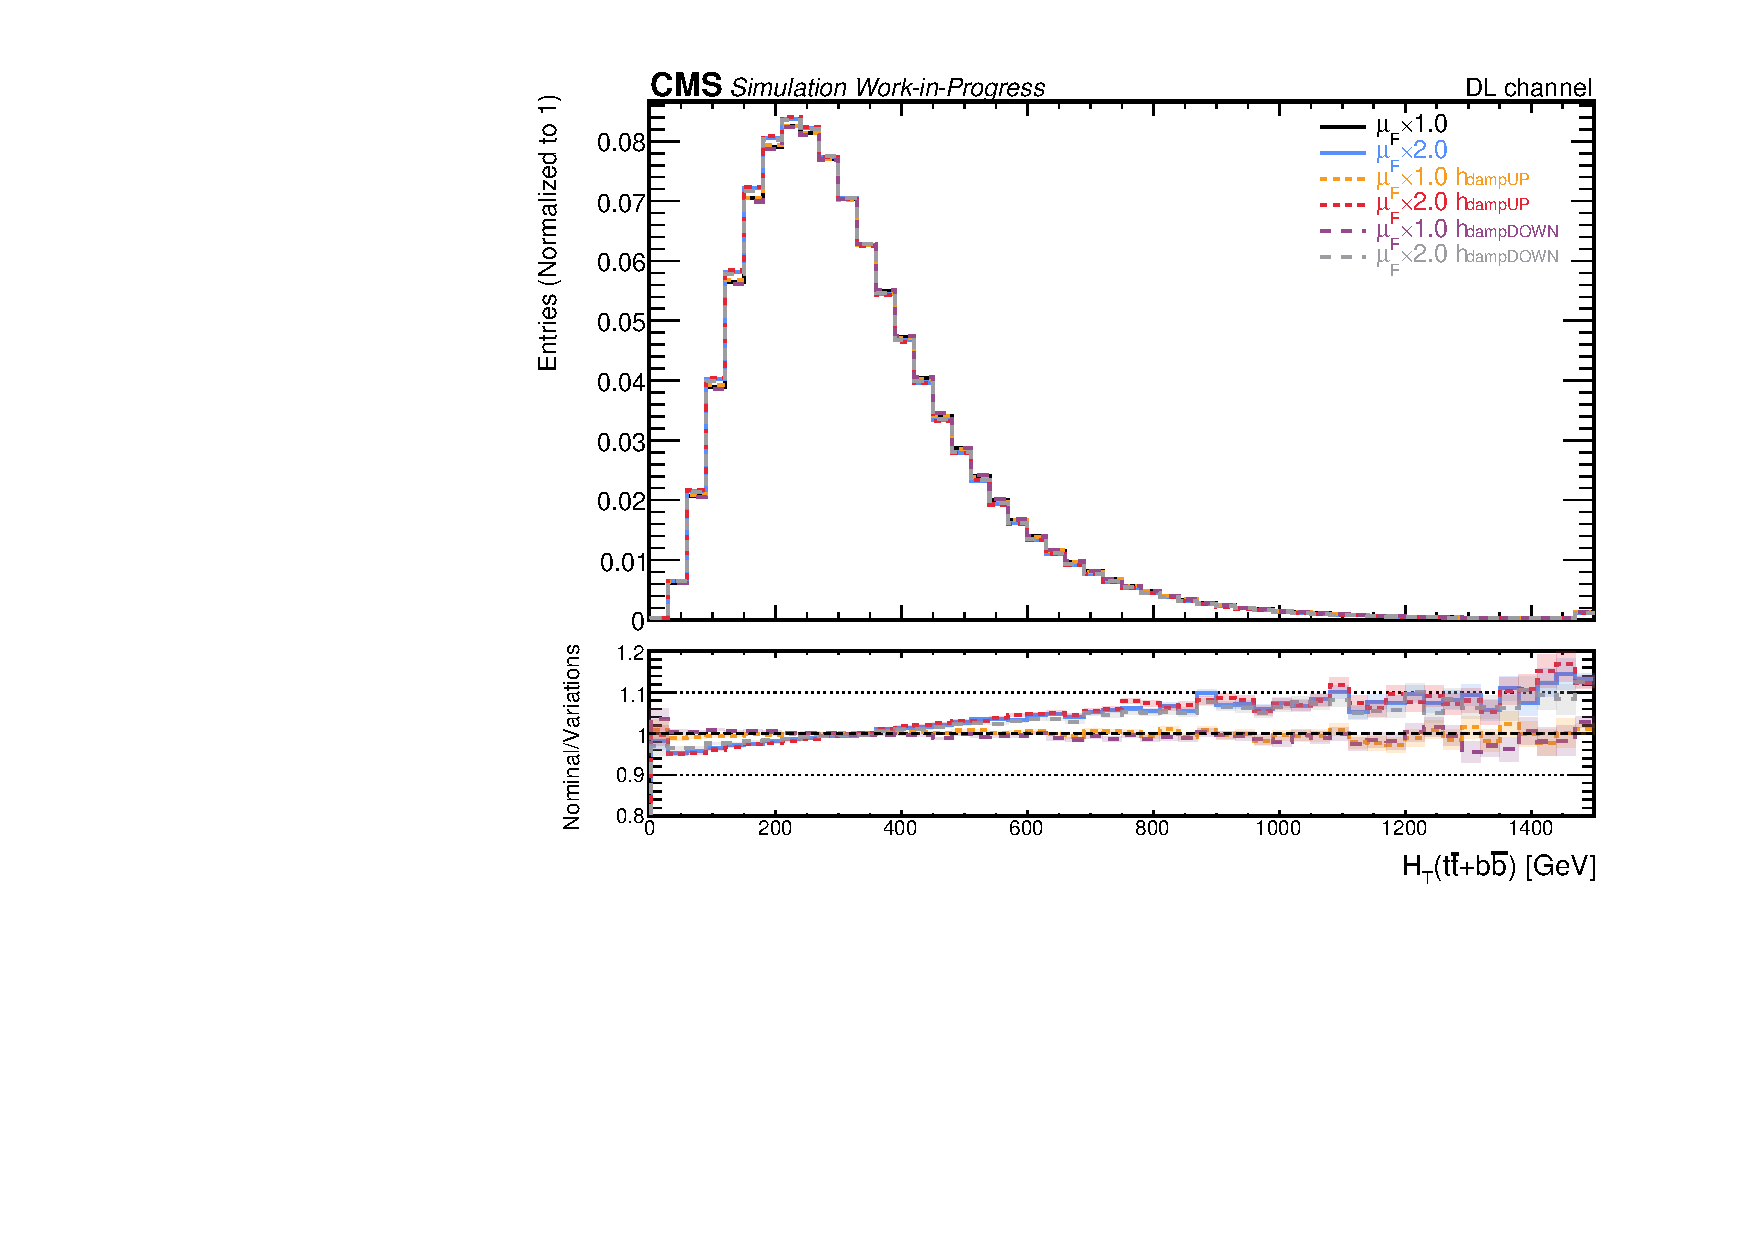
\includegraphics[width= 1.1\linewidth]{DL/ratio_Ht_hist.pdf}
        \caption{}
        \label{subfig:HT(ttbb)_DL}
    \end{subfigure}
    \caption{Distributions of (a) invariant mass and (b) H$_{\text{T}}$ of the t$\overline{\text{t}}$+b$\overline{\text{b}}$ system for the six different settings used in the simulation. The lower panel shows the ratio of the nominal setting to the variations. The shaded bands represent statistical uncertainties. The last bins contain the overflow events.}
    \label{fig:ttbb_DL}
\end{figure}
\begin{figure}[H]
    \centering
    \begin{subfigure}{0.49\textwidth}
        \centering
        \includegraphics[width= 1.1\linewidth]{DL/ratio_leptons_pt.pdf}
        \caption{}
        \label{subfig:pt(leptons)_DL}        
    \end{subfigure}
    \hfill
    \begin{subfigure}{0.49\linewidth}
        \centering
        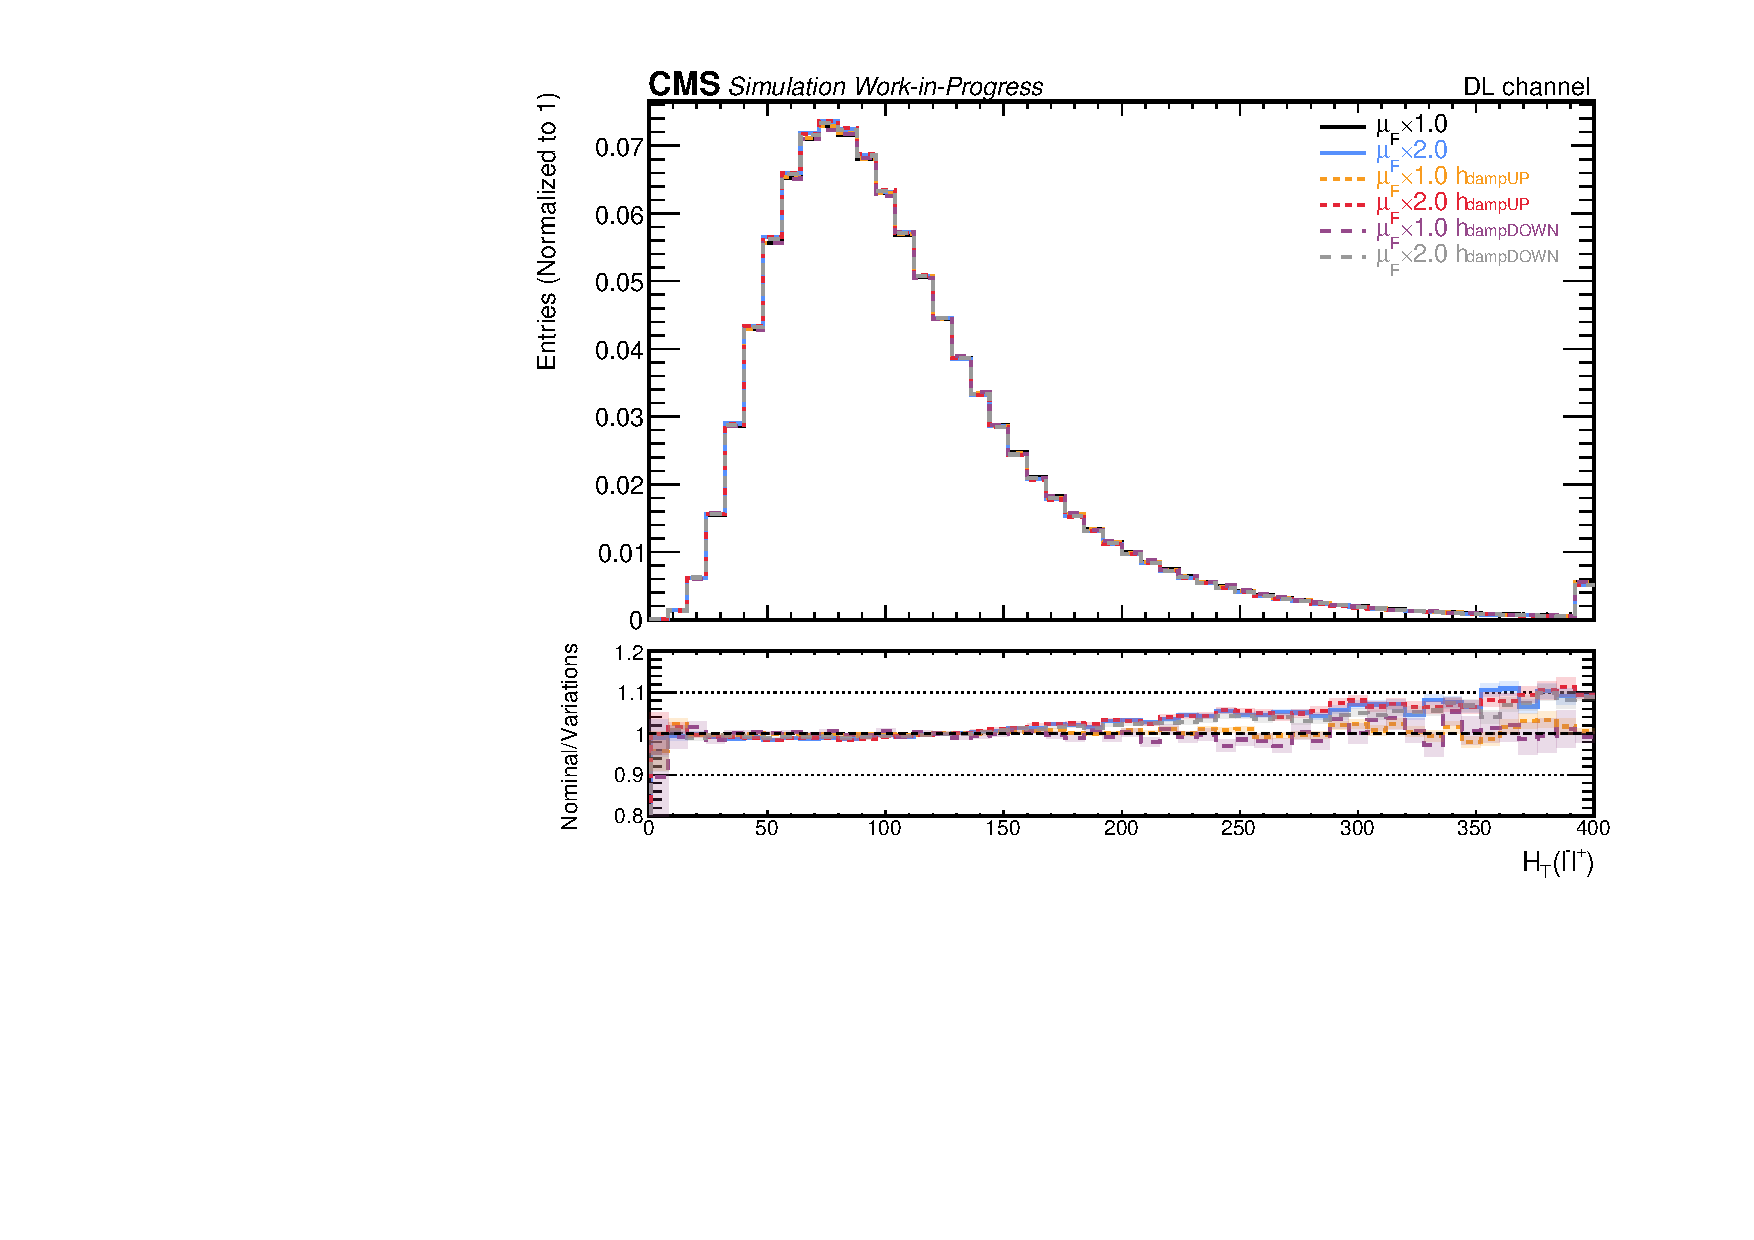
\includegraphics[width= 1.1\linewidth]{DL/ratio_ll_system_HT.pdf}
        \caption{}
        \label{subfig:HT(ll)_DL}
    \end{subfigure}
    \caption{Distribution of (a) the transverse momentum of all the leptons (charged and neutral) and (b) the H$_{\text{T}}$ of $\ell^-\ell^+$ system for the six different settings used in the simulation. The lower panel shows the ratio of the nominal setting to the variations. The shaded bands represent statistical uncertainties. The last bins contain the overflow events.}
    \label{fig:leptons_DL}
\end{figure}
\begin{figure}[H]
    \centering
    \begin{subfigure}{0.32\textwidth}
        \centering
        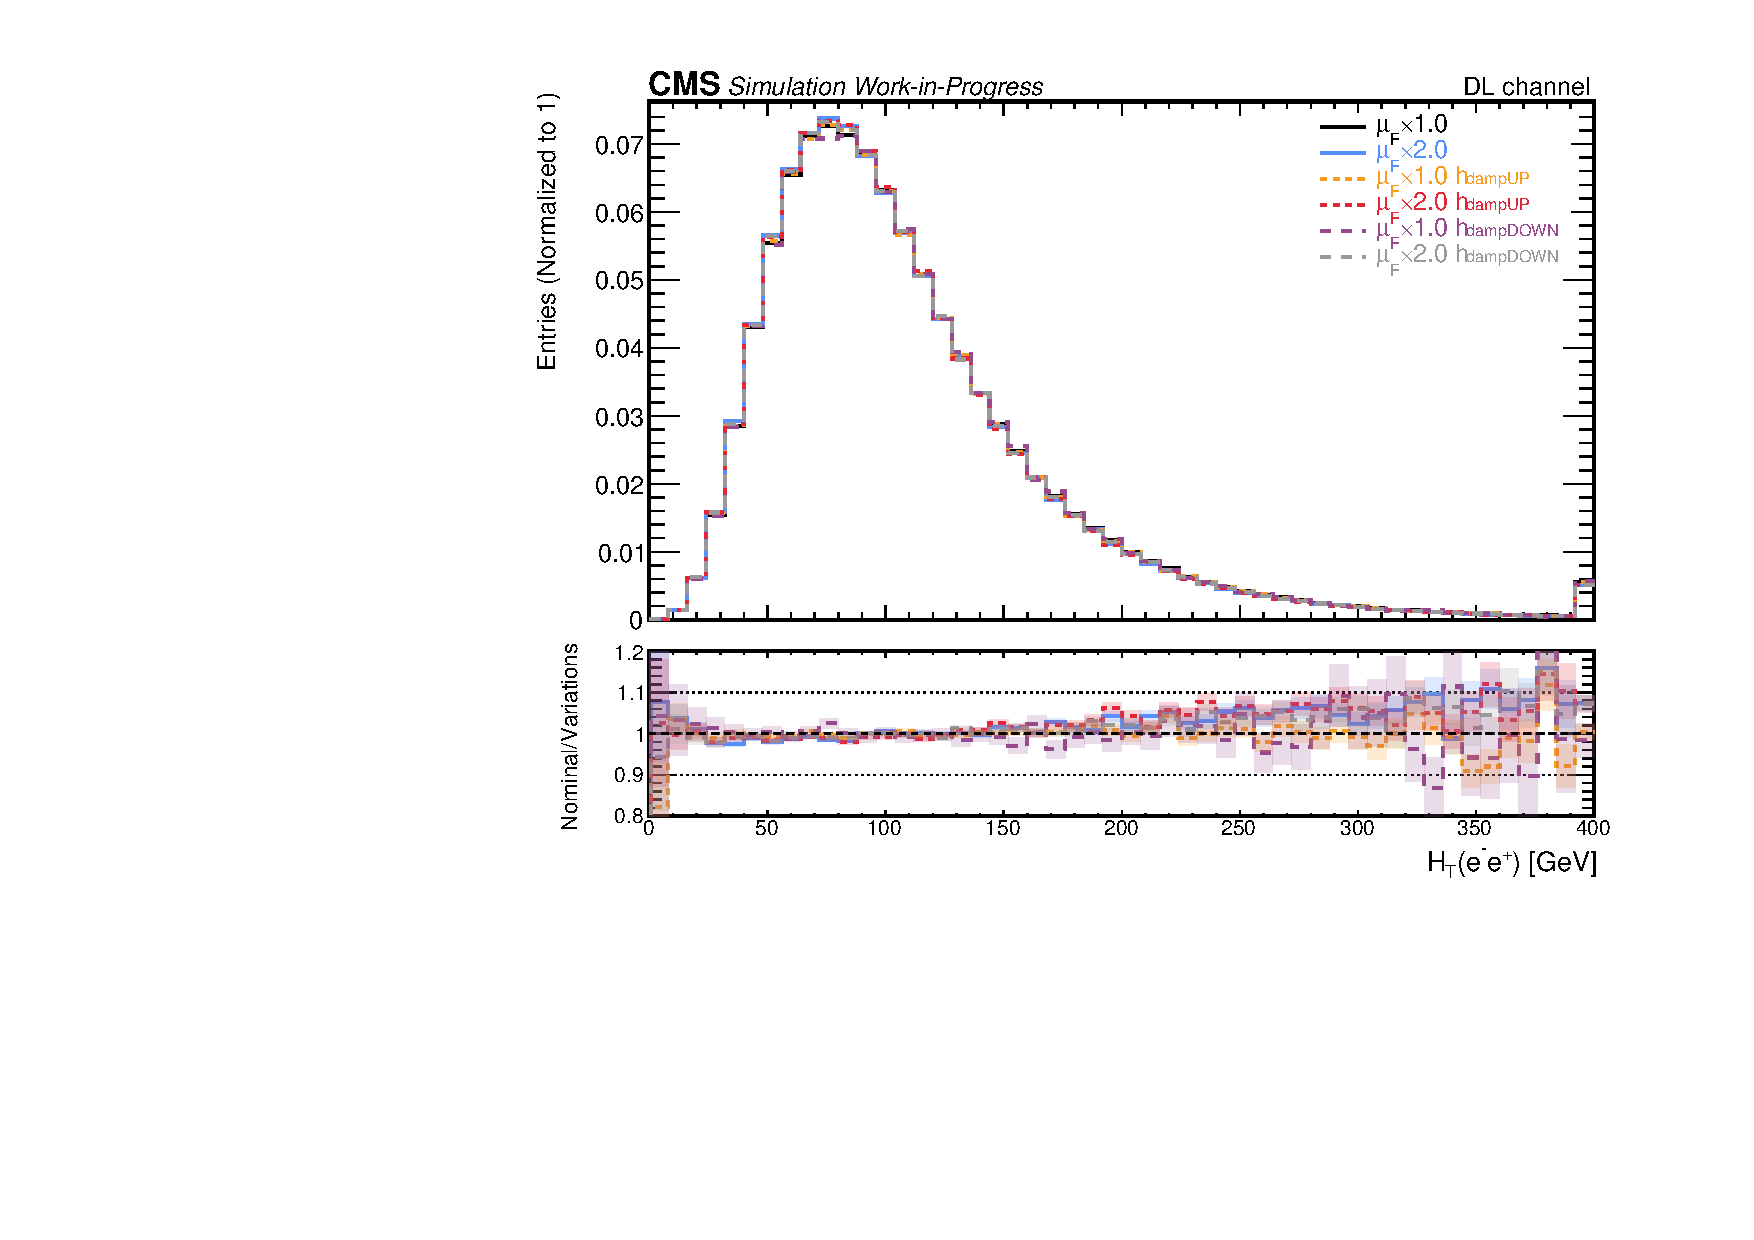
\includegraphics[width= 1.0\linewidth]{DL/ratio_ee_system_HT.pdf}
        \caption{}
        \label{subfig:HT(ee)_DL}
    \end{subfigure}
\hfill
    \begin{subfigure}{0.32\textwidth}
        \centering
        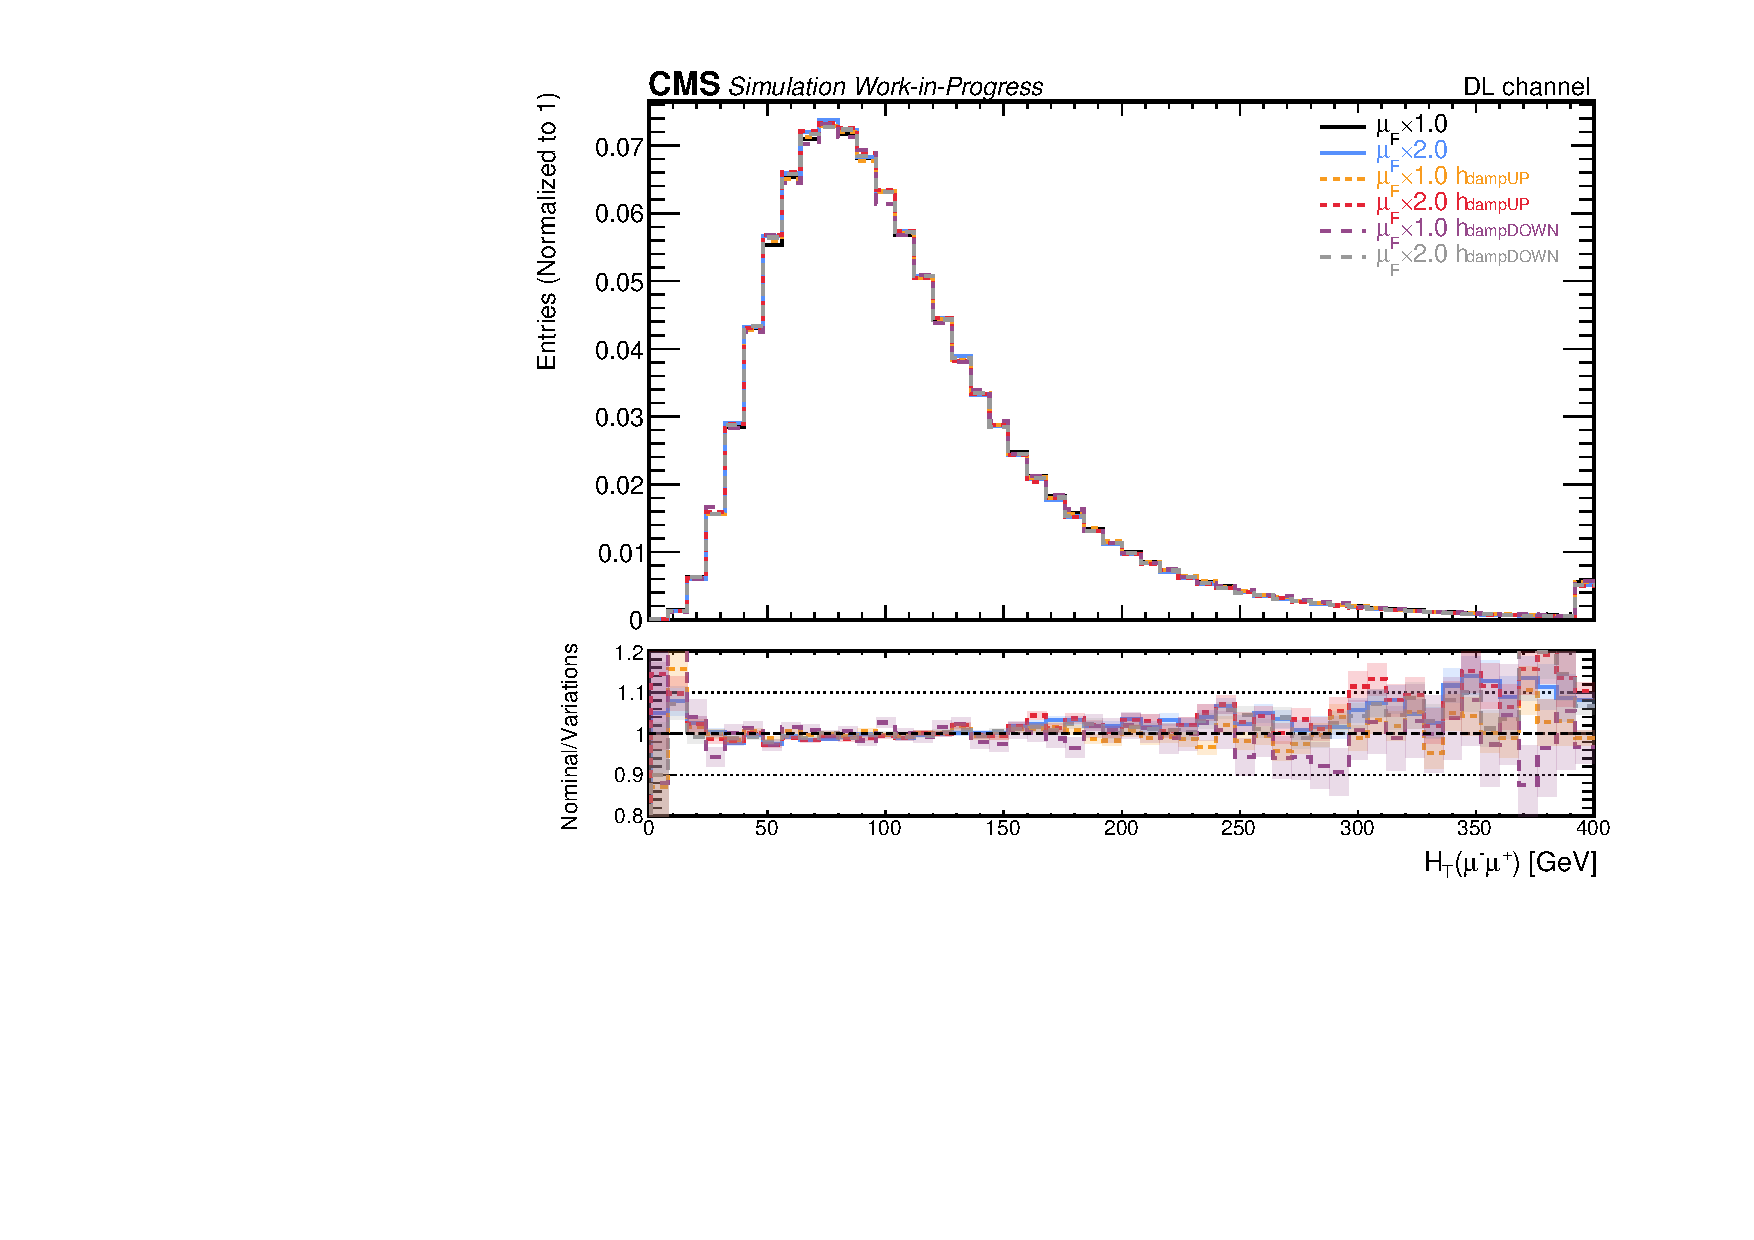
\includegraphics[width= 1.0\linewidth]{DL/ratio_mm_system_HT.pdf}
        \caption{}
        \label{subfig:HT(mm)_DL}
    \end{subfigure}
\hfill
    \begin{subfigure}{0.32\textwidth}
        \centering
        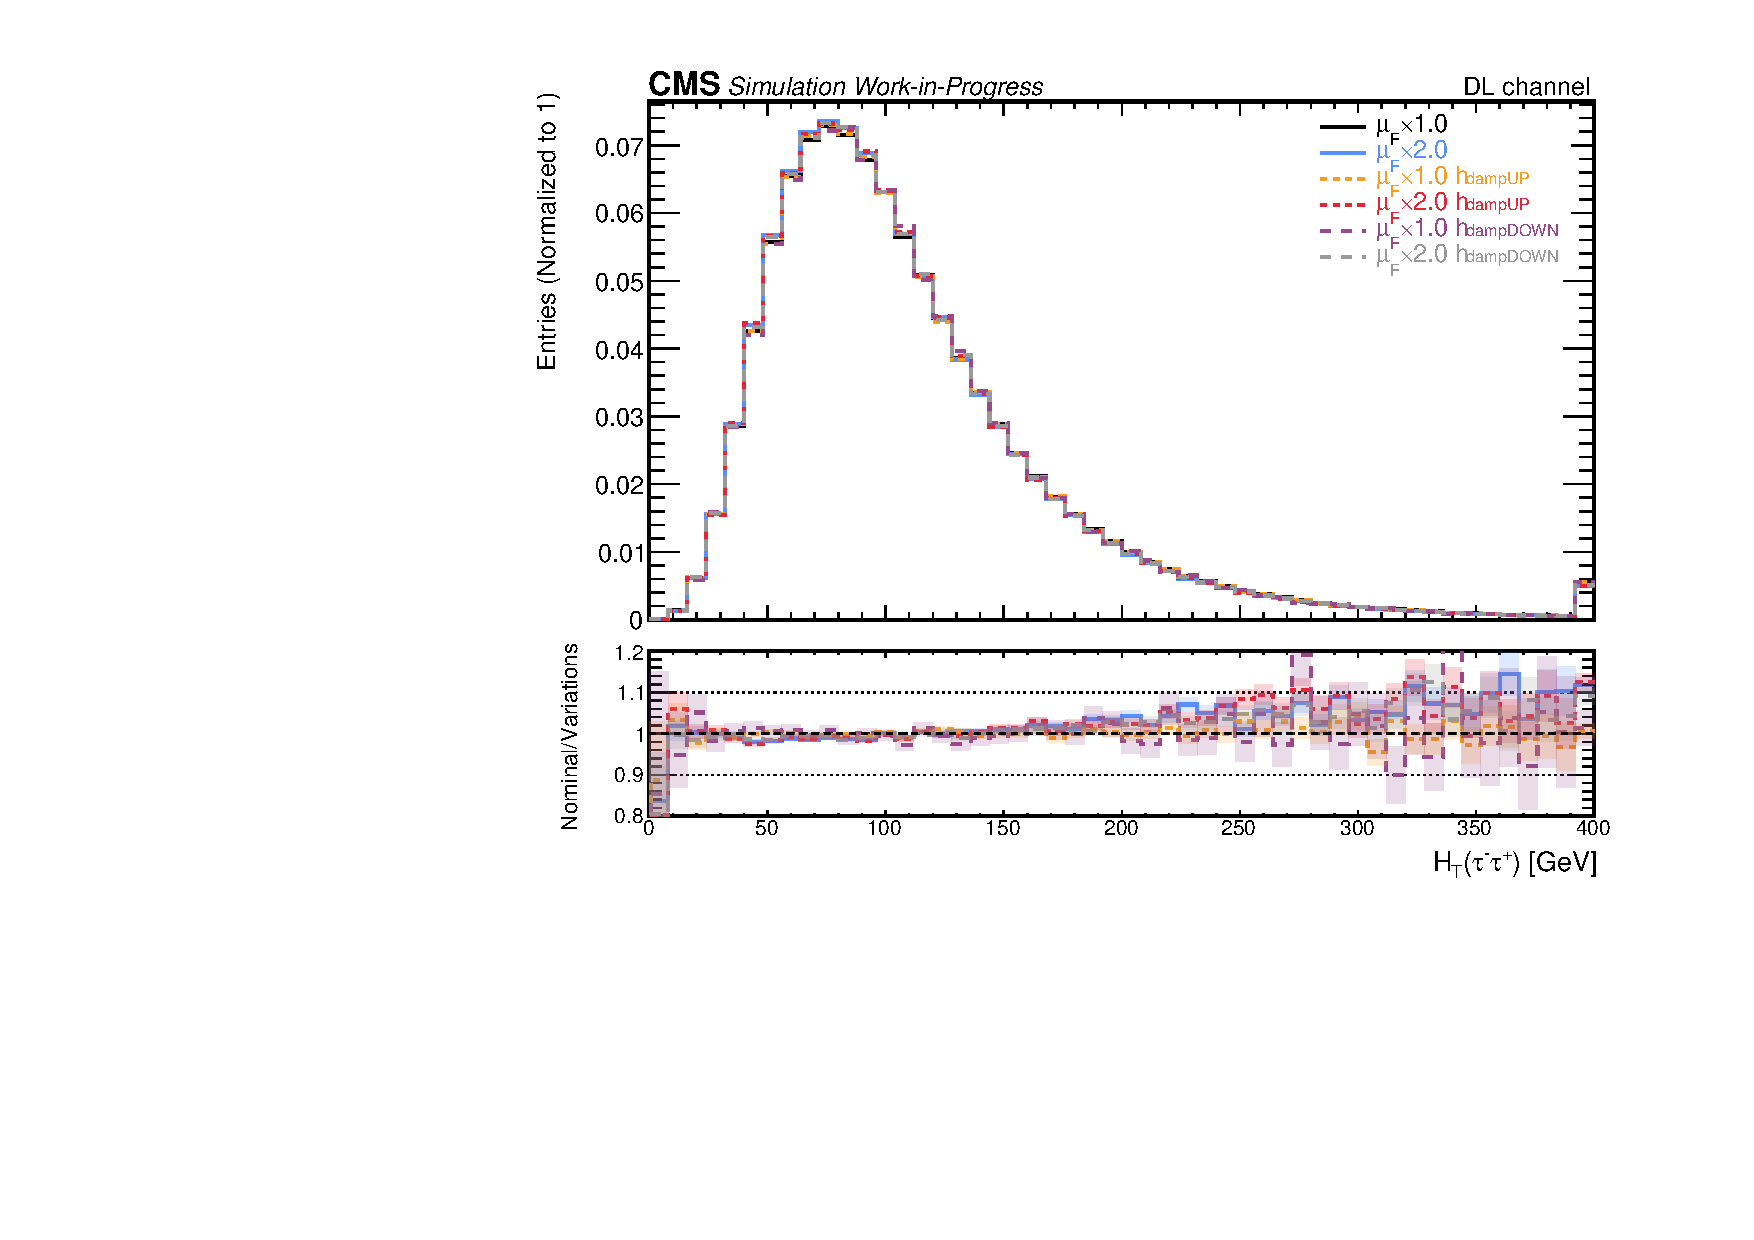
\includegraphics[width= 1.0\linewidth]{DL/ratio_tautau_system_HT.pdf}
        \caption{}
        \label{subfig:HT(tt)_DL}
    \end{subfigure}

    \vspace{0.2cm}

    \begin{subfigure}{0.32\textwidth}
        \centering
        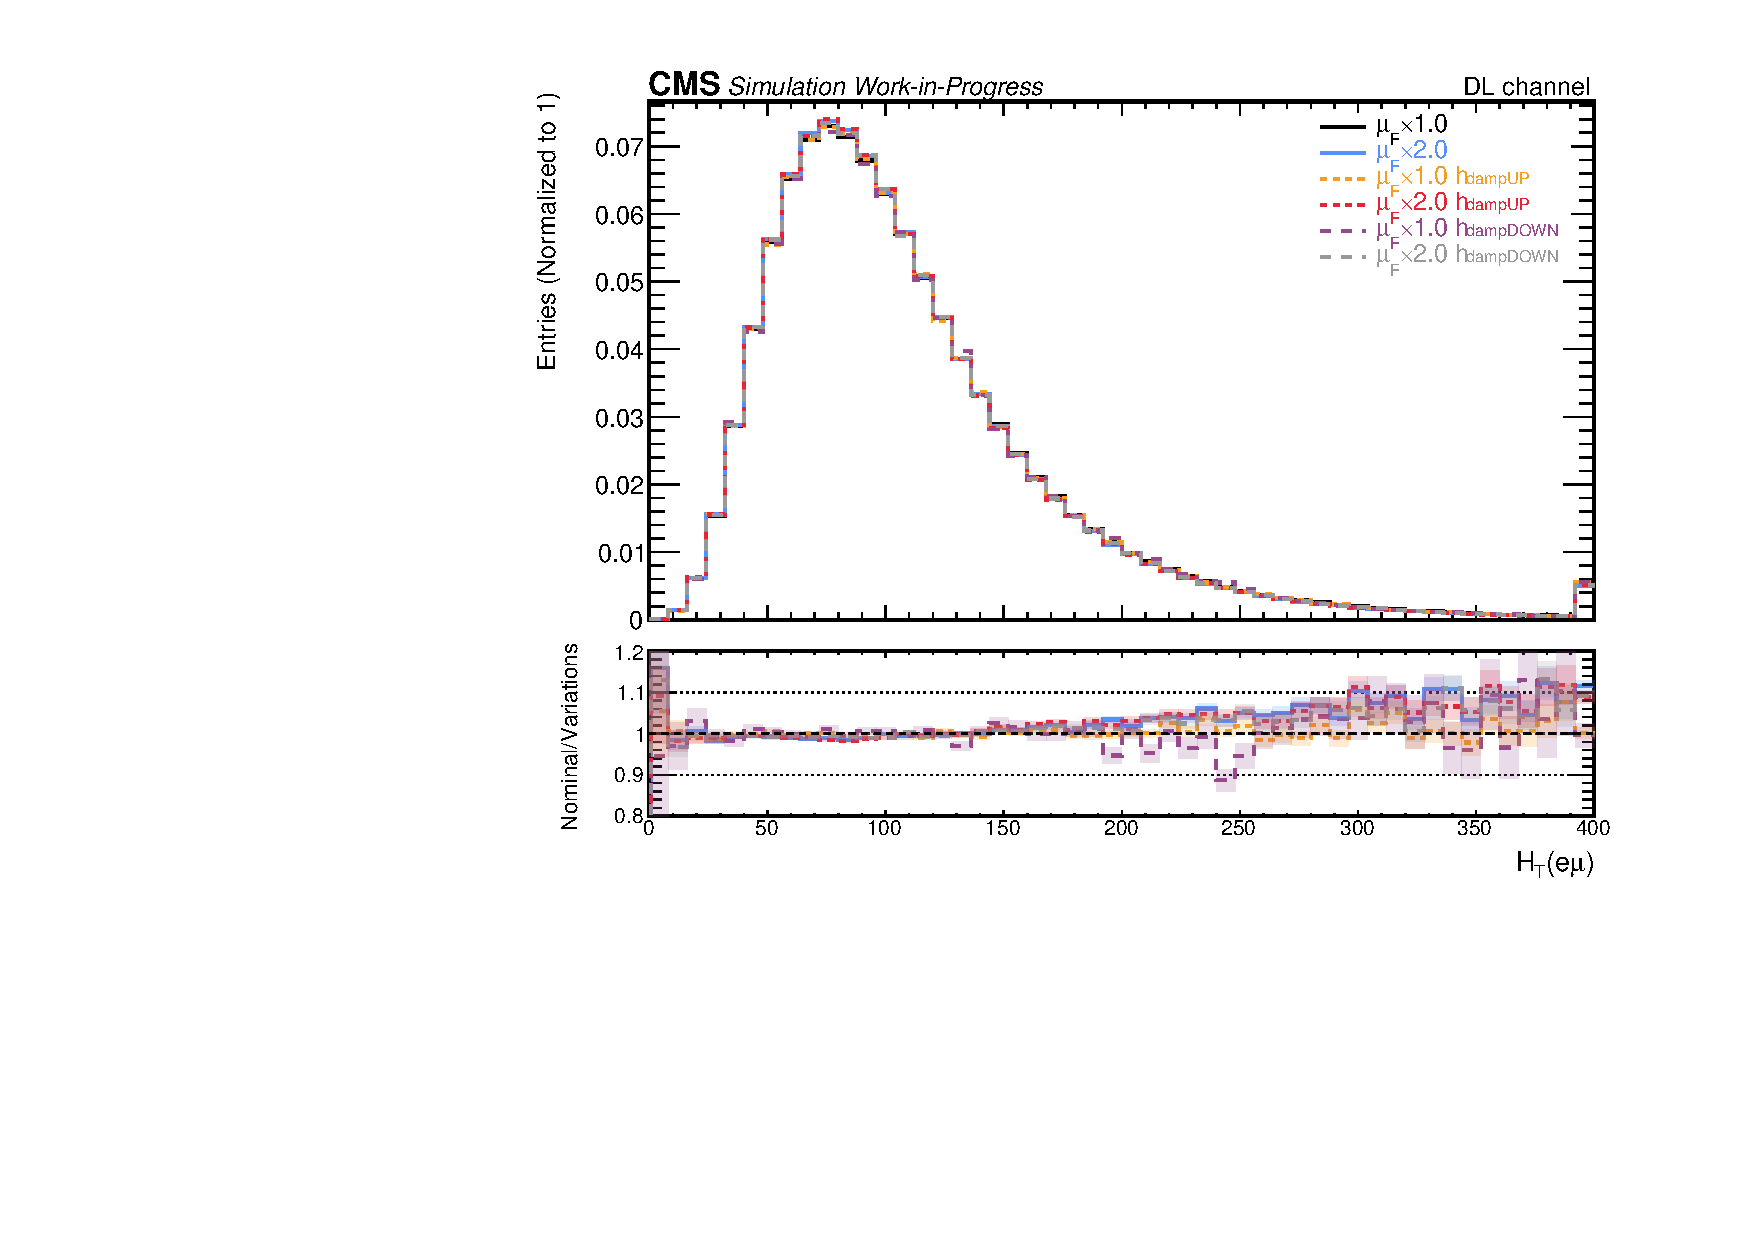
\includegraphics[width= 1.0\linewidth]{DL/ratio_em_system_HT.pdf}
        \caption{}
        \label{subfig:HT(em)_DL}
    \end{subfigure}
\hfill
    \begin{subfigure}{0.32\textwidth}
        \centering
        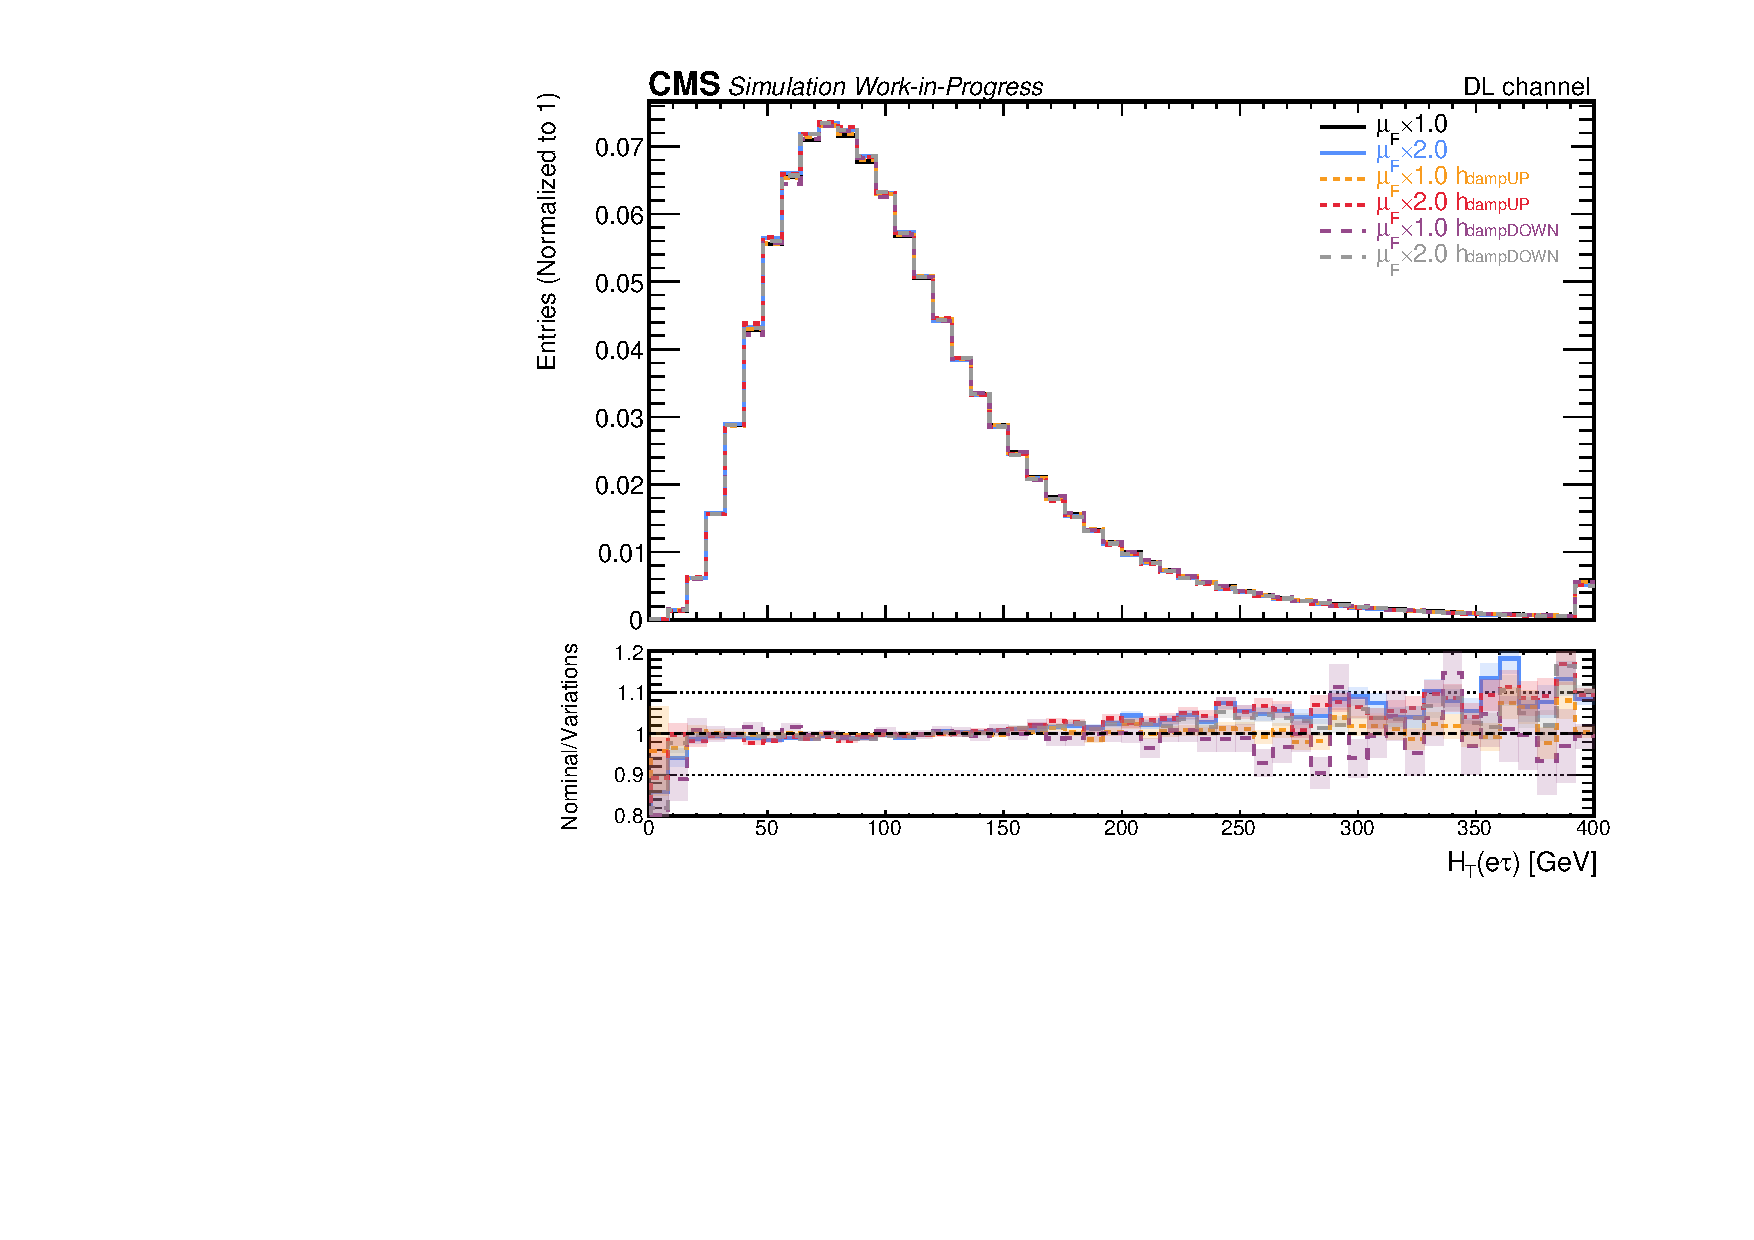
\includegraphics[width= 1.0\linewidth]{DL/ratio_et_system_HT.pdf}
        \caption{}
        \label{subfig:HT(et)_DL}
    \end{subfigure}
\hfill
    \begin{subfigure}{0.32\textwidth}
        \centering
        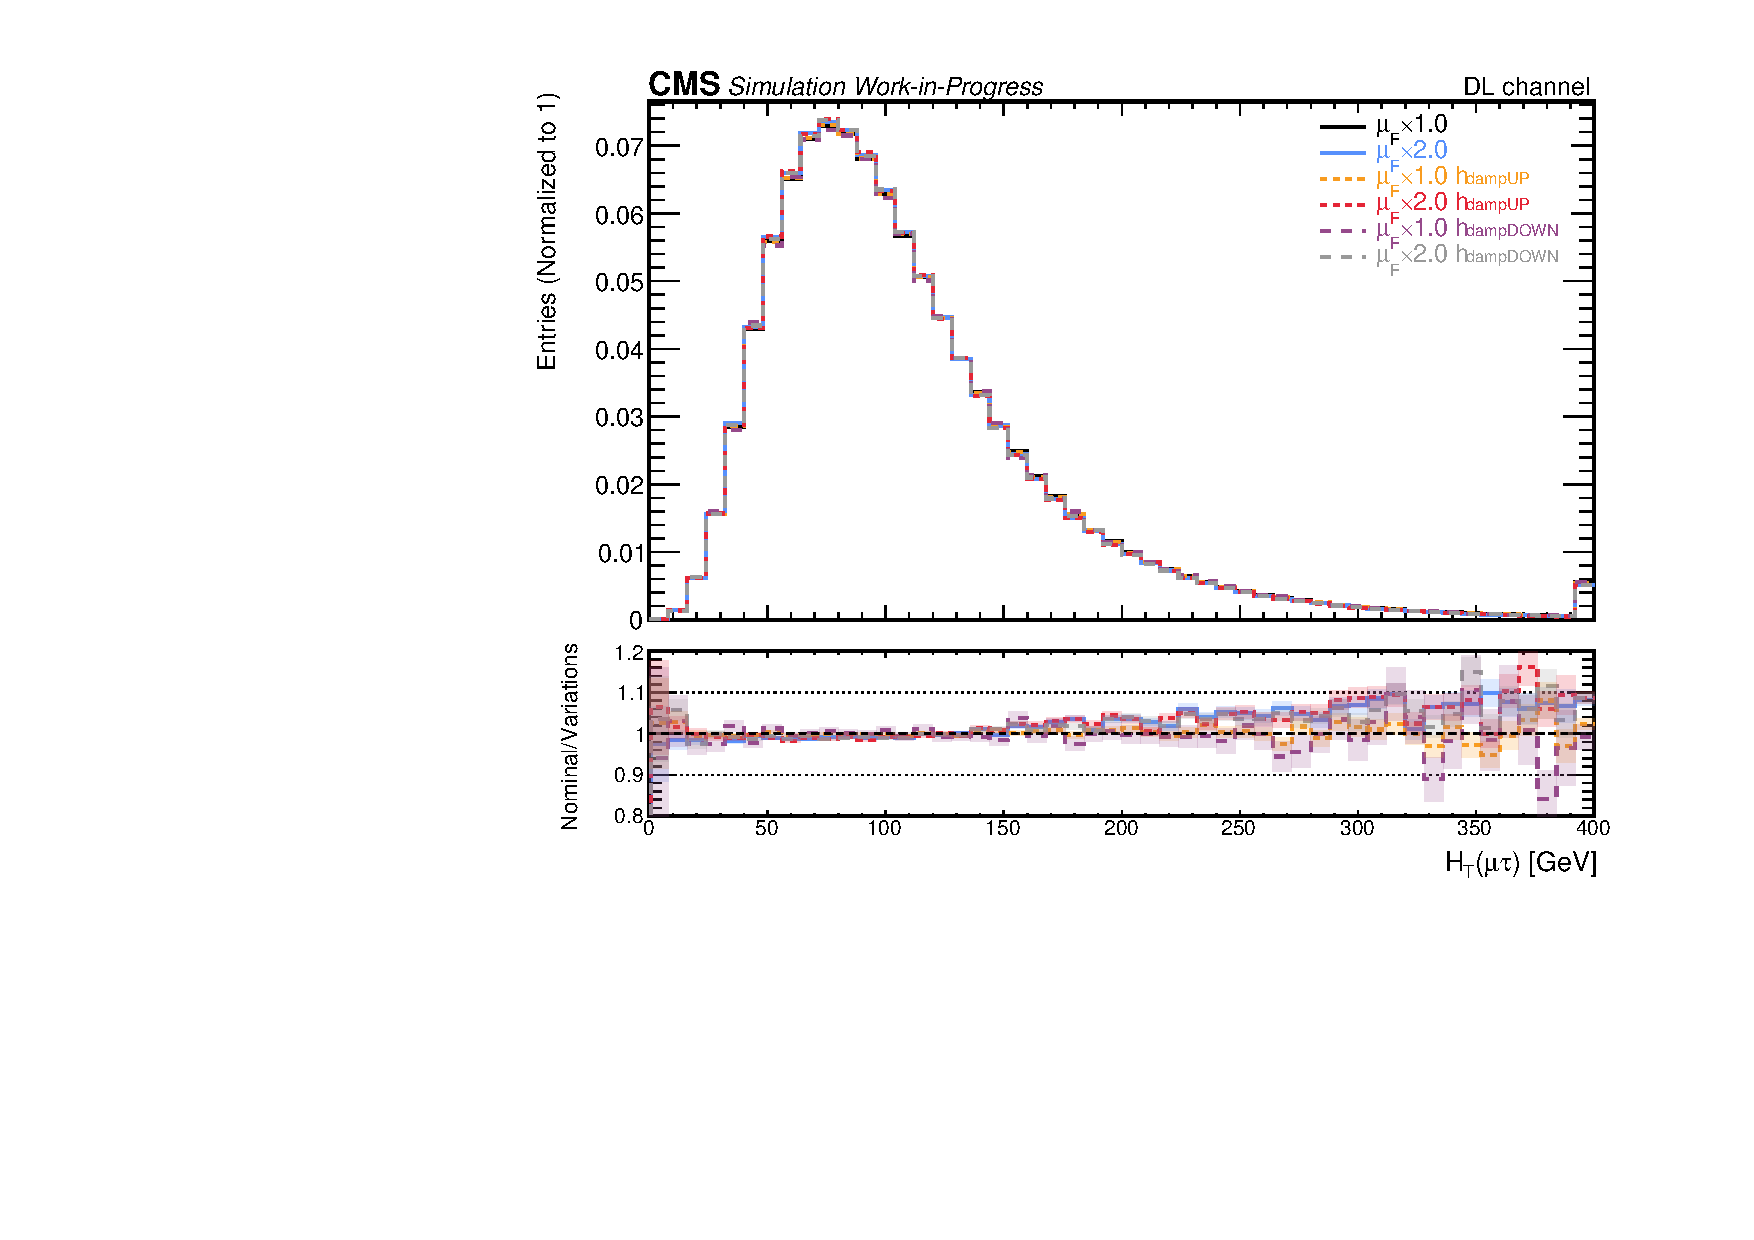
\includegraphics[width= 1.0\linewidth]{DL/ratio_mt_system_HT.pdf}
        \caption{}
        \label{subfig:HT(mt)_DL}
    \end{subfigure}
    \caption{Distribution of H$_\text{T}$ for (a) $e^-e^+$, (b) $\mu^-\mu^+$, (c) $\tau^-\tau^+$, (d) $e\mu$ (e) $e\tau$ and (f) $\mu\tau$ systems for the six different settings used in the simulation. The lower panel shows the ratio of the nominal setting to the variations. The shaded bands represent statistical uncertainties. }
    \label{fig:HT(ll_all)_DL}
\end{figure}
\indent The results, for the combination of the two separate systems, i.e. the t$\overline{\text{t}}$ and the prompt b$\overline{\text{b}}$ systems, are shown in Figure \ref{fig:ttbb_DL}. It is clear that, the effect of the  factorization scale remains the same in the distribution of H$_\text{T}$ for the inclusive t$\overline{\text{t}}$+b$\overline{\text{b}}$ system. The same can be said, also, for its invariant mass, with the effect, even being, stronger for values above 2000 GeV. In fact, for these high values of the invariant mass, there is also a separation between the different damping settings, reaching up to $20 \%$ difference for the sample with hdampDOWN and $\mu_F \times 2$ settings.\\
\indent As for the other final state particles, which in this case are leptons, the results are shown in Figure \ref{fig:leptons_DL}. Similarly to the previous results from the quarks, both the transverse momentum of leptons (\ref{subfig:pt(leptons)_DL}) and H$_{\text{T}}$ of the $\ell^-\ell^+$ system (\ref{subfig:HT(ll)_DL}) are sensitive to the change of the factorization scale.\\
For completeness, the distributions of the H$_{\text{T}}$ variable for the six different leptons combinations are presented in Figure \ref{fig:HT(ll_all)_DL}. The results are similar with the combination of all, but due to this separation, there is low statistics in high H$_{\text{T}}$ values, resulting in some bigger fluctuations.\\
\indent Finally, the last particle of interest is the hardest emission generated from the {\fontfamily{bch}\fontshape{sc}\selectfont{Powheg}} method. We would expect that this extra light jet will be the most sensitive particle to the choice of  h$_{damp}$, since it regulates the hardness of this radiation. As it is shown in Figure \ref{fig:radiation_DL}, this is true for the hdampDOWN variation. For both factorization scales, the hdampDOWN variation is consistently above, in the ratio plot. To be more specific, this effect appears to be larger in case of the $\mu_F \times 1$, reaching up to 8 \% difference in the high $p_{\text{T}}$ spectrum. Of course, the change of the factorization scale again affects significantly the distribution for high $p_{\text{T}}$ values, where with the combination of the hdampDOWN, we observe almost 12 \% difference.
\begin{figure}[htb!]
    \centering
    \includegraphics[width= 0.54\linewidth]{DL/ratio_radiation_pt.pdf}
    \caption{Distribution of the transverse momentum of the extra light jet for the six different settings used in the simulation. The lower panel shows the ratio of the nominal setting to the variations. The shaded bands represent statistical uncertainties. The last bins contain the overflow events.}
    \label{fig:radiation_DL}
\end{figure}
\newpage
\subsection{\label{SL}Semileptonic channel}
\noindent In the semileptonic channel, as the name suggests, only one W boson decays into leptons with the other decaying hadronically. The appearance of more jets in the final state makes this channel a little more challenging to model in comparison with the DL channel, but due to the significantly larger branching ratio, it is more promising for the search of the Yukawa coupling.\\
\indent As was the case for the DL, the observables that were found to be more sensitive to the choice of the different settings are the transverse momentum and H$_{\text{T}}$. In Figure \ref{fig:HT_SL}, the distributions of H$_{\text{T}}$ for the t$\overline{\text{t}}$ and the two different b$\overline{\text{b}}$ systems are presented, while in Figure \ref{fig:pt_SL}, the transverse momentum for t/$\overline{\text{t}}$ and the b/$\overline{\text{b}}$ quarks is presented.\\
\begin{figure}[H]
    \centering
    \begin{subfigure}{0.49\textwidth}
        \centering
        \includegraphics[width= 1.05\linewidth]{SL/ratio_tt_system_HT.pdf}
        \caption{}
        \label{subfig:HT(ttbar)_SL}
    \end{subfigure}
    \hfill
    \begin{subfigure}{0.49\textwidth}
        \centering
        \includegraphics[width= 1.05\linewidth]{SL/ratio_prompt_bs_HT.pdf}
        \caption{}
        \label{subfig:HT(bbbar_prompt)_SL}
    \end{subfigure}
    \hfill
    \begin{subfigure}{0.49\textwidth}
        \centering
        \includegraphics[width= 1.05\linewidth]{SL/ratio_bs_from_top_HT.pdf}
        \caption{}
        \label{subfig:HT(bbbar)_SL}
    \end{subfigure}
    \caption{Distribution of H$_{\text{T}}$ for (a) t$\overline{\text{t}}$, (b) prompt b$\overline{\text{b}}$ and (c) b$\overline{\text{b}}$, originating from top quarks, systems for the six different settings used in the simulation. The lower panel shows the ratio of the nominal setting to the variations. The shaded bands represent statistical uncertainties. The last bins contain the overflow events.}
    \label{fig:HT_SL}
\end{figure}
\indent With no surprise the results are identical to the ones in the DL channel. There is a strong trend in the high p$_{\text{T}}$ spectrum for the $\mu_F \times 2$ setting, especially for the t/$\overline{\text{t}}$ quarks in Figure \ref{subfig:pt(t,tbar)_SL}. The same can be said for the H$_{\text{T}}$ distributions for the quark-antiquark systems with the exception of the prompt b$\overline{\text{b}}$ system in Fig. \ref{subfig:HT(bbbar_prompt)_SL}. There are little to no deviations for the different h$_{\text{damp}}$ parameters for the two different factorization scales.\\
\begin{figure}[H]
    \centering
    \begin{subfigure}{0.49\textwidth}
        \centering
        \includegraphics[width= 1.1\linewidth]{SL/ratio_ttbar_pt.pdf}
        \caption{}
        \label{subfig:pt(t,tbar)_SL}        
    \end{subfigure}
    \hfill
    \begin{subfigure}{0.49\linewidth}
        \centering
        \includegraphics[width= 1.1\textwidth]{SL/ratio_b_all_pt.pdf}
        \caption{}
        \label{subfig:pt(b_all)_SL}
    \end{subfigure}
    \caption{Distribution of the transverse momentum of (a) the t/$\overline{\text{t}}$ and (b) the b/$\overline{\text{b}}$ quarks for the six different settings used in the simulation. The lower panel shows the ratio of the nominal setting to the variations. The shaded bands represent statistical uncertainties. The last bins contain the overflow events.}
    \label{fig:pt_SL}
\end{figure}




\begin{figure}[H]
    \centering
    \begin{subfigure}{0.49\textwidth}
        \centering
        \includegraphics[width= 1.1\linewidth]{SL/ratio_invariant_mass_hist.pdf}
        \caption{}
        \label{subfig:m(ttbb)_SL}        
    \end{subfigure}
    \hfill
    \begin{subfigure}{0.49\linewidth}
        \centering
        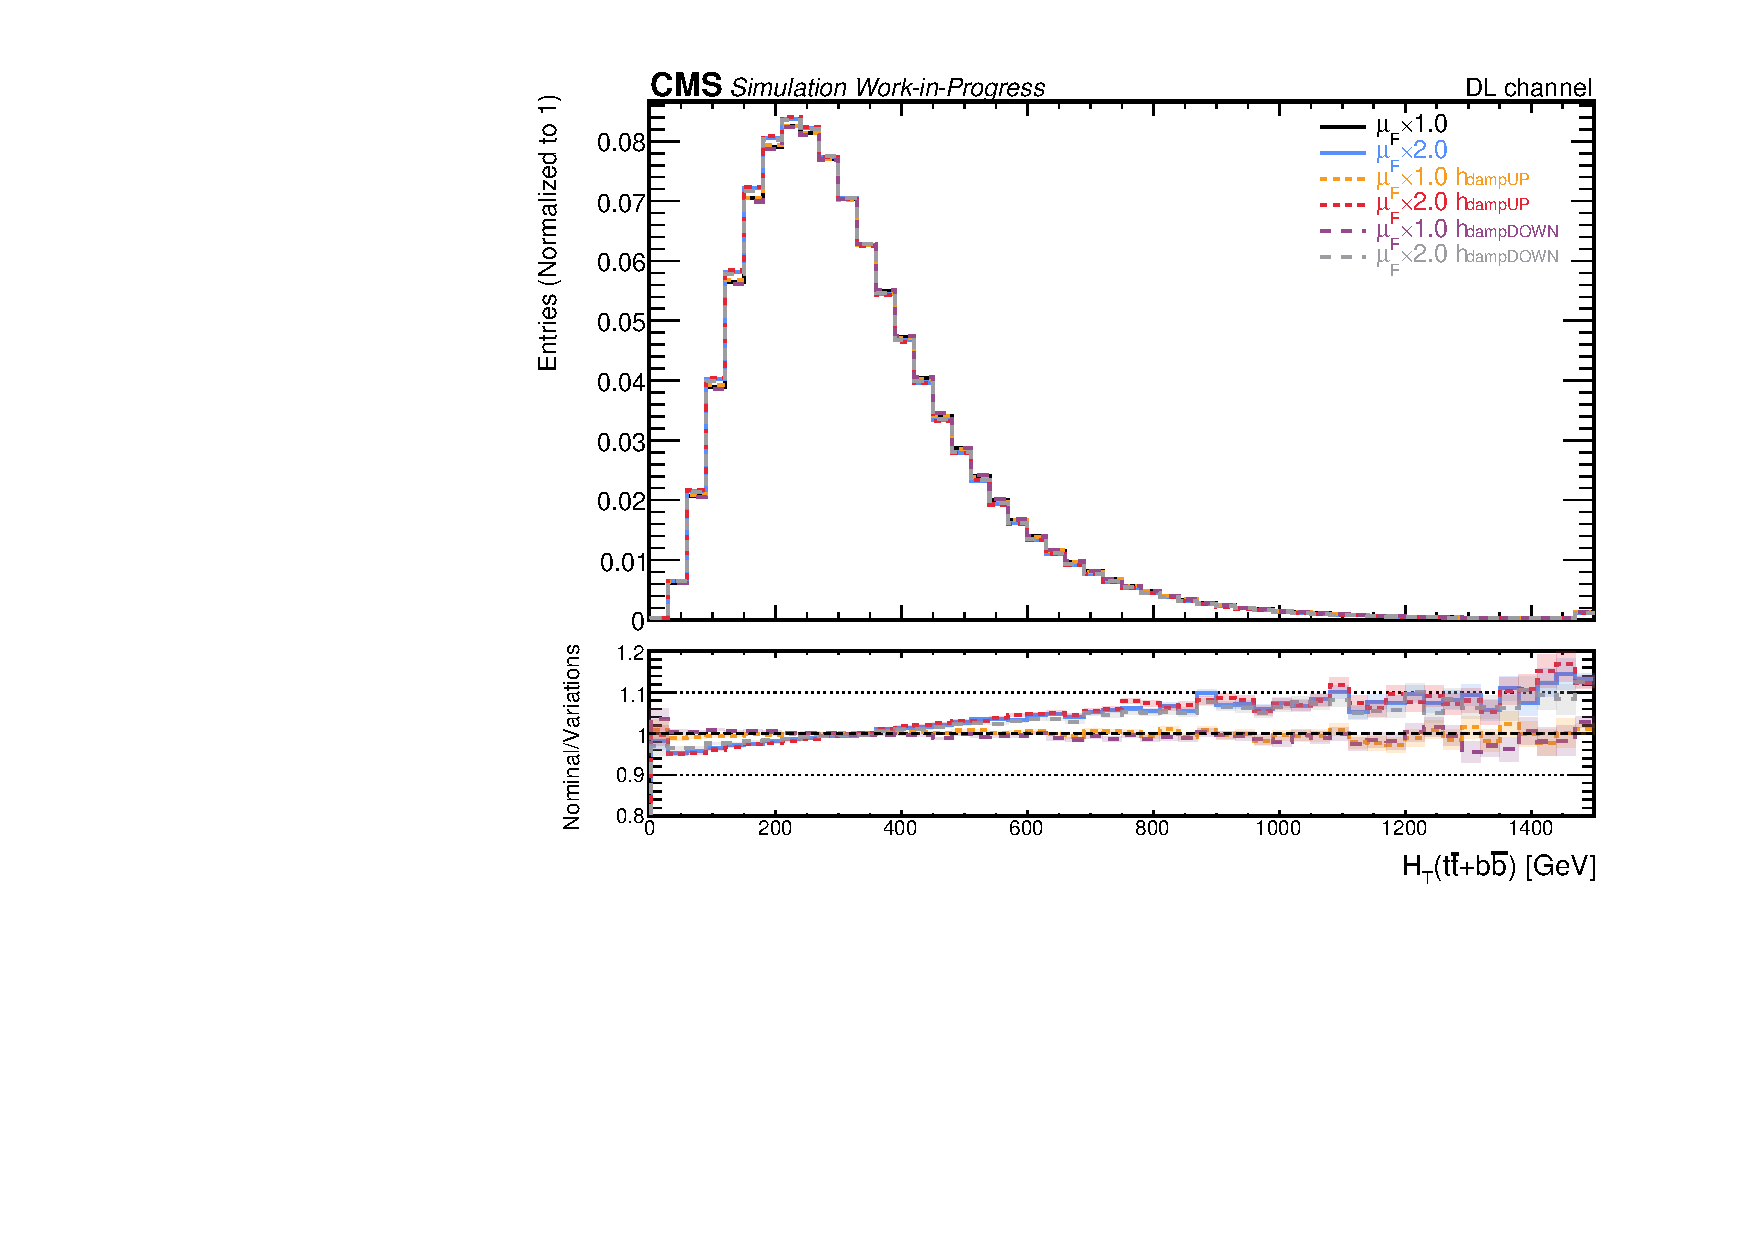
\includegraphics[width= 1.1\linewidth]{DL/ratio_Ht_hist.pdf}
        \caption{}
        \label{subfig:HT(ttbb)_SL}
    \end{subfigure}
    \caption{Distribution of (a) invariant mass and (b) H$_{\text{T}}$ for the t$\overline{\text{t}}$+b$\overline{\text{b}}$ system for the six different settings used in the simulation. The lower panel shows the ratio of the nominal setting to the variations. The shaded bands represent statistical uncertainties. The last bins contain the overflow events.}
    \label{fig:ttbb_SL}
\end{figure}
In Figure \ref{fig:ttbb_SL}, the distributions of the invariant mass and the H$_{\text{T}}$ for the t$\overline{\text{t}}$+b$\overline{\text{b}}$ system are shown. There is a strong effect for the samples with $\mu_F \times 2$ for both distributions, as was the case in the DL channel. As for the different damping parameters, there is basically no difference between them for the H$_{\text{T}}$. However, this is not the case for the invariant mass where, there are some significant deviations at very high values, especially in the case of the hdampDOWN setting 
\begin{figure}[H]
    \centering
    \begin{subfigure}{0.49\textwidth}
        \centering
        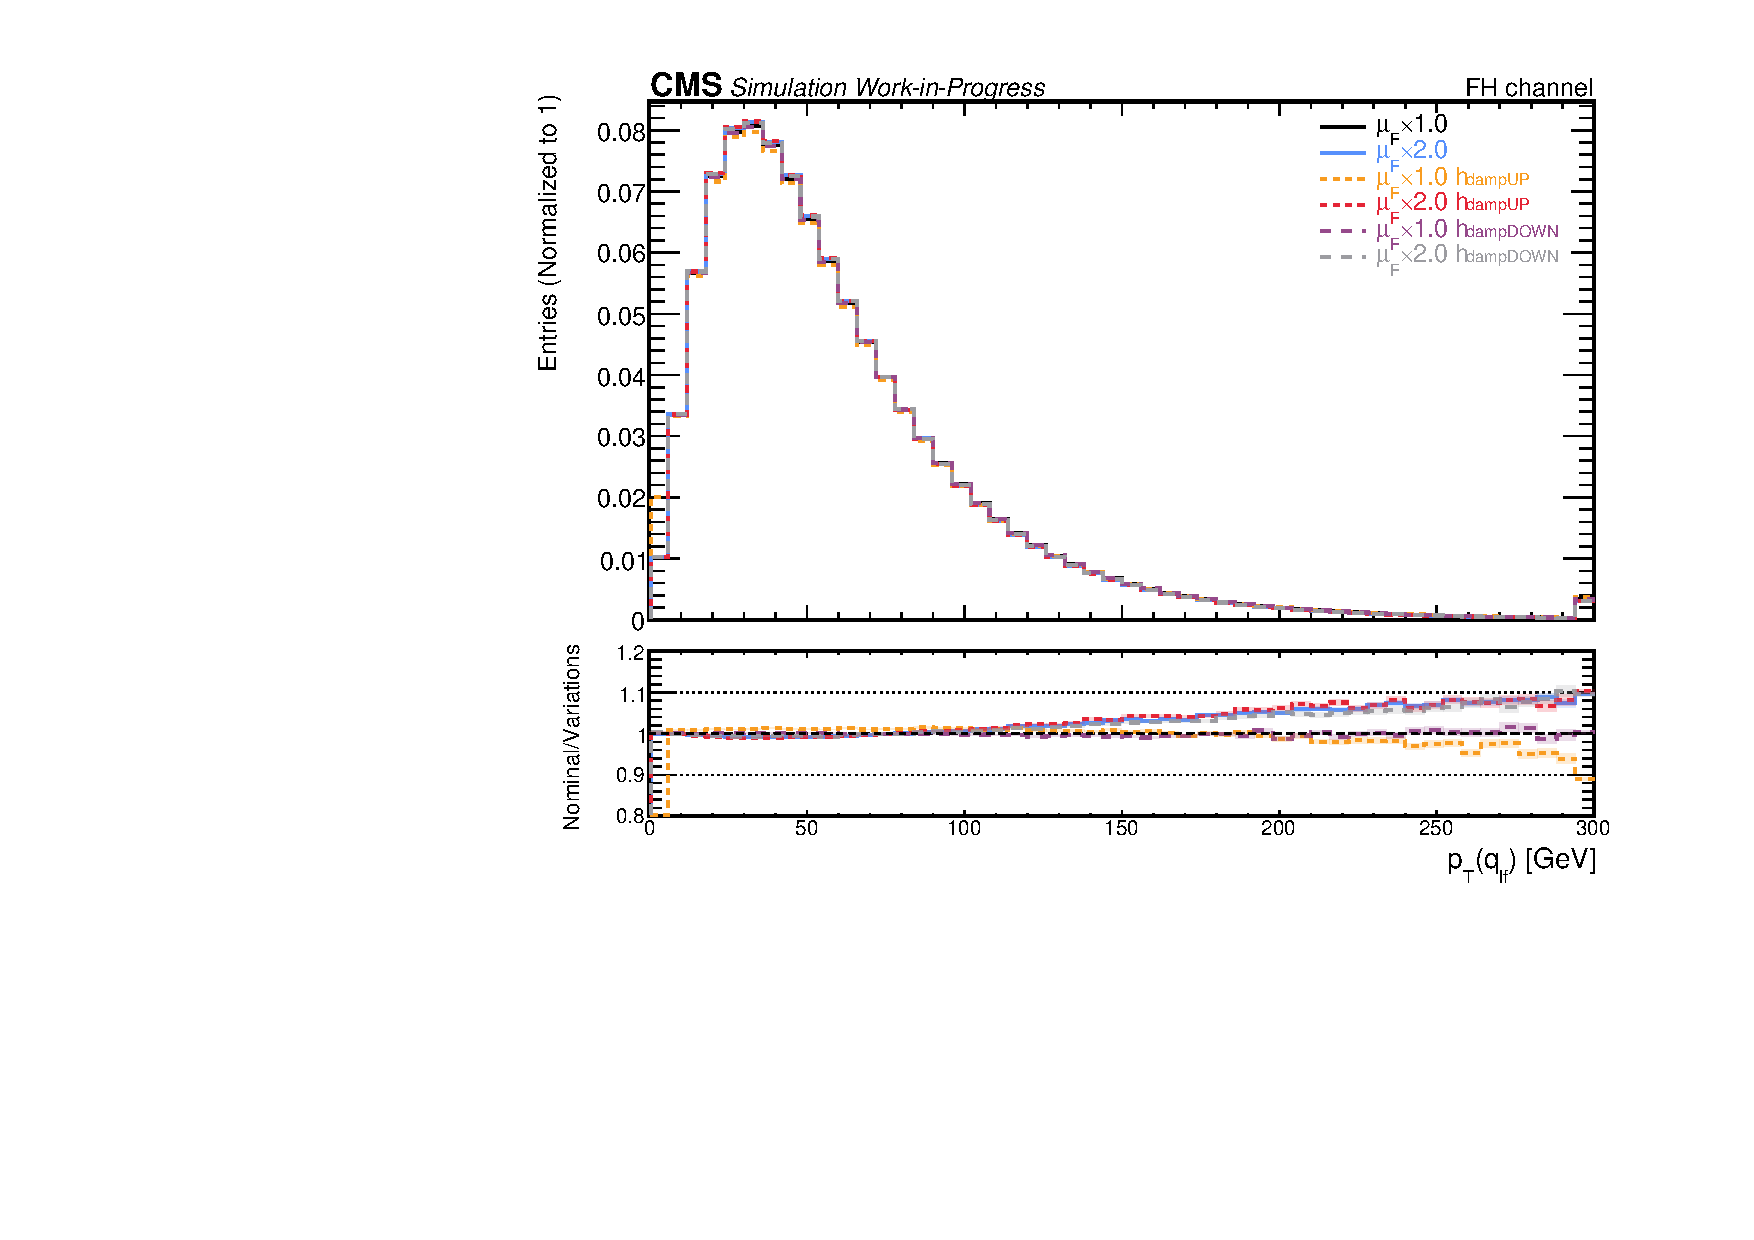
\includegraphics[width= 1.05\linewidth]{SL/ratio_quarks_pt.pdf}
        \caption{}
        \label{subfig:pt(quarks)_SL}        
    \end{subfigure}
    \hfill
    \begin{subfigure}{0.49\linewidth}
        \centering
        \includegraphics[width= 1.05\linewidth]{SL/ratio_leptons_pt.pdf}
        \caption{}
        \label{subfig:pt(leptons)_SL}
    \end{subfigure}
    \hfill
    \begin{subfigure}{0.49\linewidth}
        \centering
        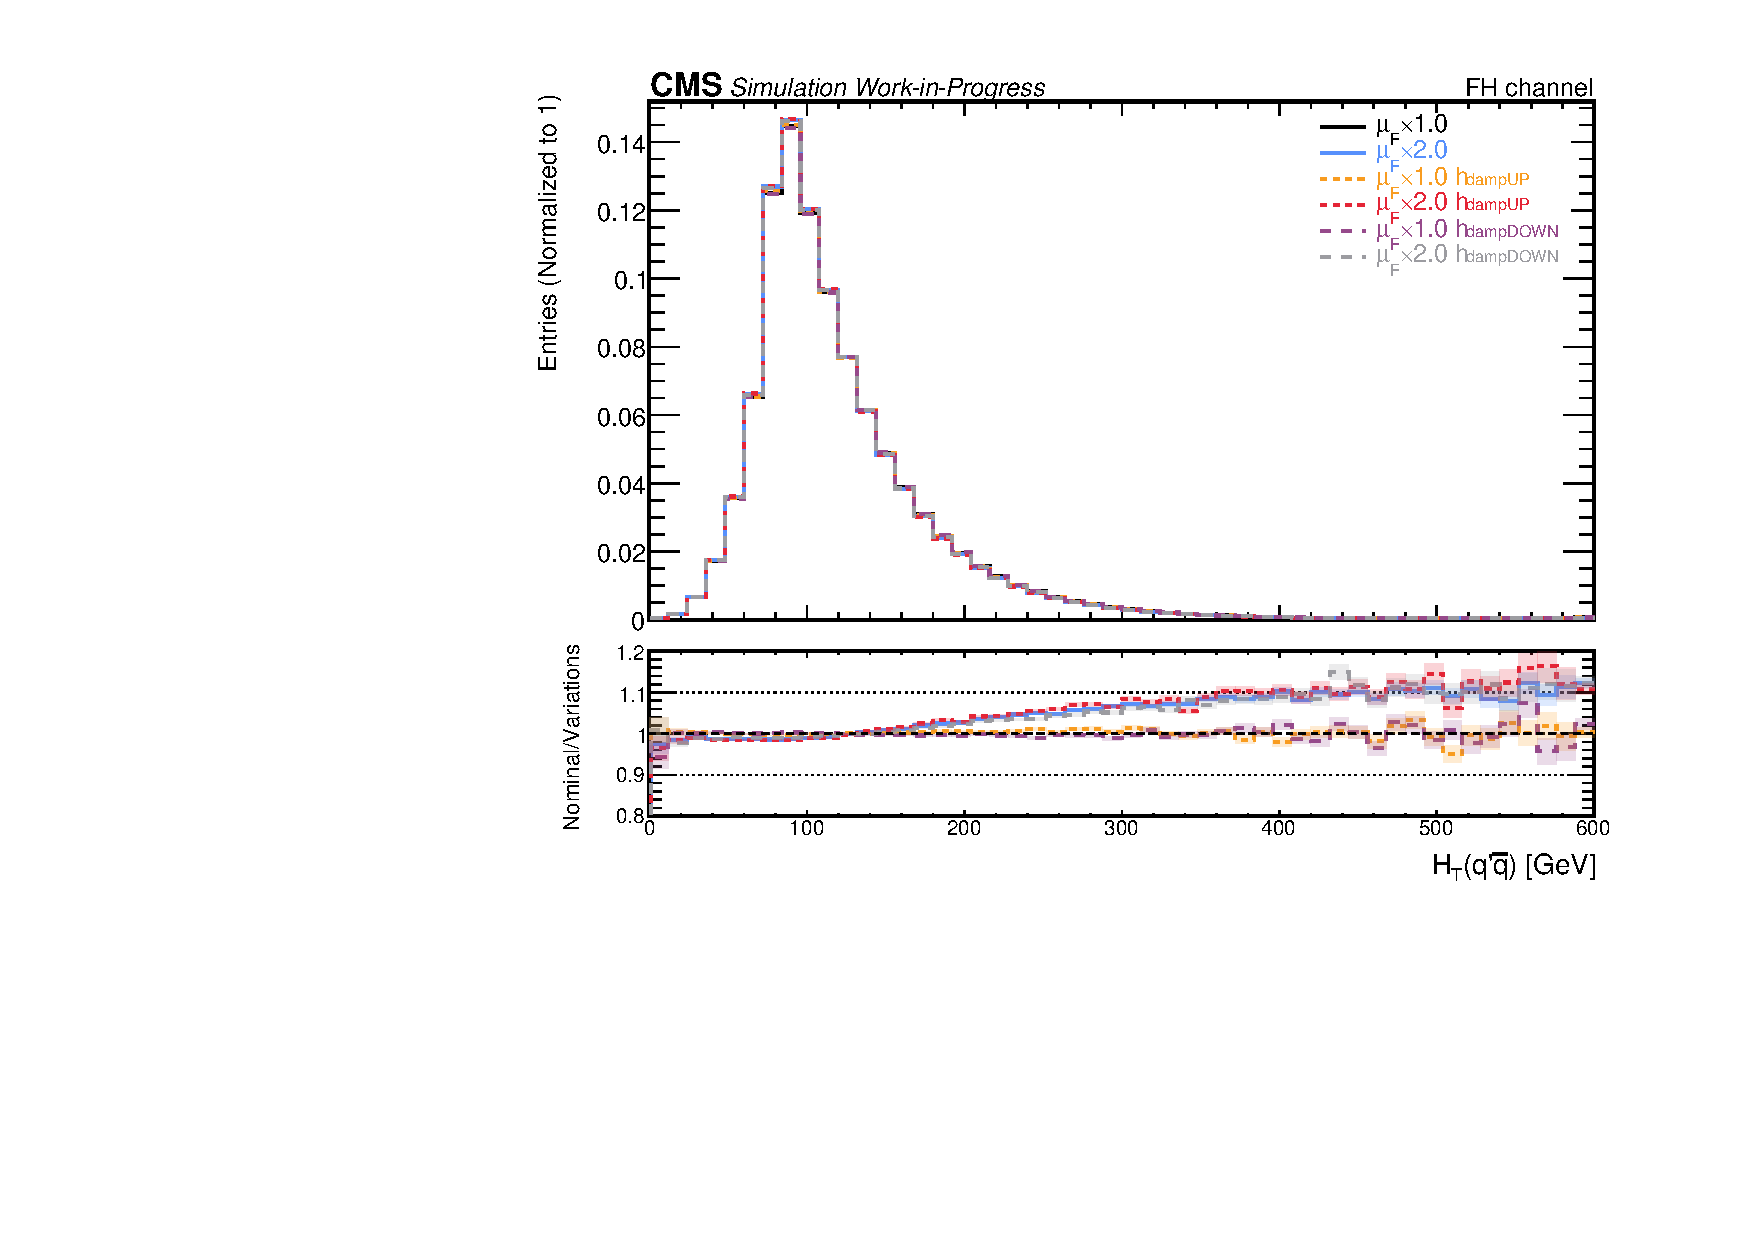
\includegraphics[width= 1.05\linewidth]{SL/ratio_quarks_system_HT.pdf}
        \caption{}
        \label{subfig:HT(qq)_SL}
    \end{subfigure}
    \caption{Distribution of the transverse momentum of (a) light flavor quarks and (b) leptons, and (c) the H$_{\text{T}}$ of $\overline{\text{q}}$q' system for the six different settings used in the simulation. The lower panel shows the ratio of the nominal setting to the variations. The shaded bands represent statistical uncertainties. The last bins contain the overflow events.}
    \label{fig:quarks_leptons_SL}
\end{figure}
\indent The difference from the DL channel, lies in the final state particles, whose variables of interest are illustrated in Figure \ref{fig:quarks_leptons_SL}. Specifically, in Figure \ref{subfig:pt(quarks)_SL} the distribution of the transverse momentum of the light flavor quarks originating from W boson decays is presented, whereas in Figure \ref{subfig:pt(leptons)_SL} the corresponding plot for the leptons is shown. In both figures, we observe the same behavior as before, significant difference towards higher p$_{\text{T}}$ values for $\mu_F \times 2$ with very small deviations from the different $h_{\text{damp}}$ settings. The same can be said also for the H$_{\text{T}}$ of the $\overline{\text{q}}$q' systems originating from the hadronic W decay presented in Figure \ref{subfig:HT(qq)_SL}. The separation of this plot into the four different quark-antiquark pairs combinations is depicted in Figure \ref{fig:quarks_SL}. It is obvious, that the two Cabibbo suppressed quark-antiquark pairs, in the two bottom plots (\ref{subfig:HT(us)_SL}, \ref{subfig:HT(cd)_SL}), have very low statistics, resulting in constant fluctuations. The other two plots (\ref{subfig:HT(ud)_SL}, \ref{subfig:HT(cs)_SL}), as it is expected have the same trend as the aggregated plot.\\
% Angular Separation plot
% \begin{figure}[H]
%     \centering
%     \begin{subfigure}{0.49\textwidth}
%         \centering
%         \includegraphics[width= 1.1\linewidth]{SL/ratio_tt_system_dR.pdf}
%         \caption{}
%         \label{subfig:dR(ttbar)_SL}        
%     \end{subfigure}
%     \hfill
%     \begin{subfigure}{0.49\linewidth}
%         \centering
%         \includegraphics[width= 1.1\linewidth]{SL/ratio_prompt_bs_dR.pdf}
%         \caption{}
%         \label{subfig:dR(bbbar_prompt)_SL}
%     \end{subfigure}
%     \caption{Distribution of the angular separation of (a) t$\overline{\text{t}}$ and (b) prompt b$\overline{\text{b}}$ systems for the six different settings used in the simulation. The lower panel shows the ratio of the nominal setting to the variations. The shaded bands represent statistical uncertainties. The last bins contain the overflow events.}
%     \label{fig:dR_SL}
% \end{figure}

\begin{figure}[H]
    \centering
    \begin{subfigure}{0.49\textwidth}
        \centering
        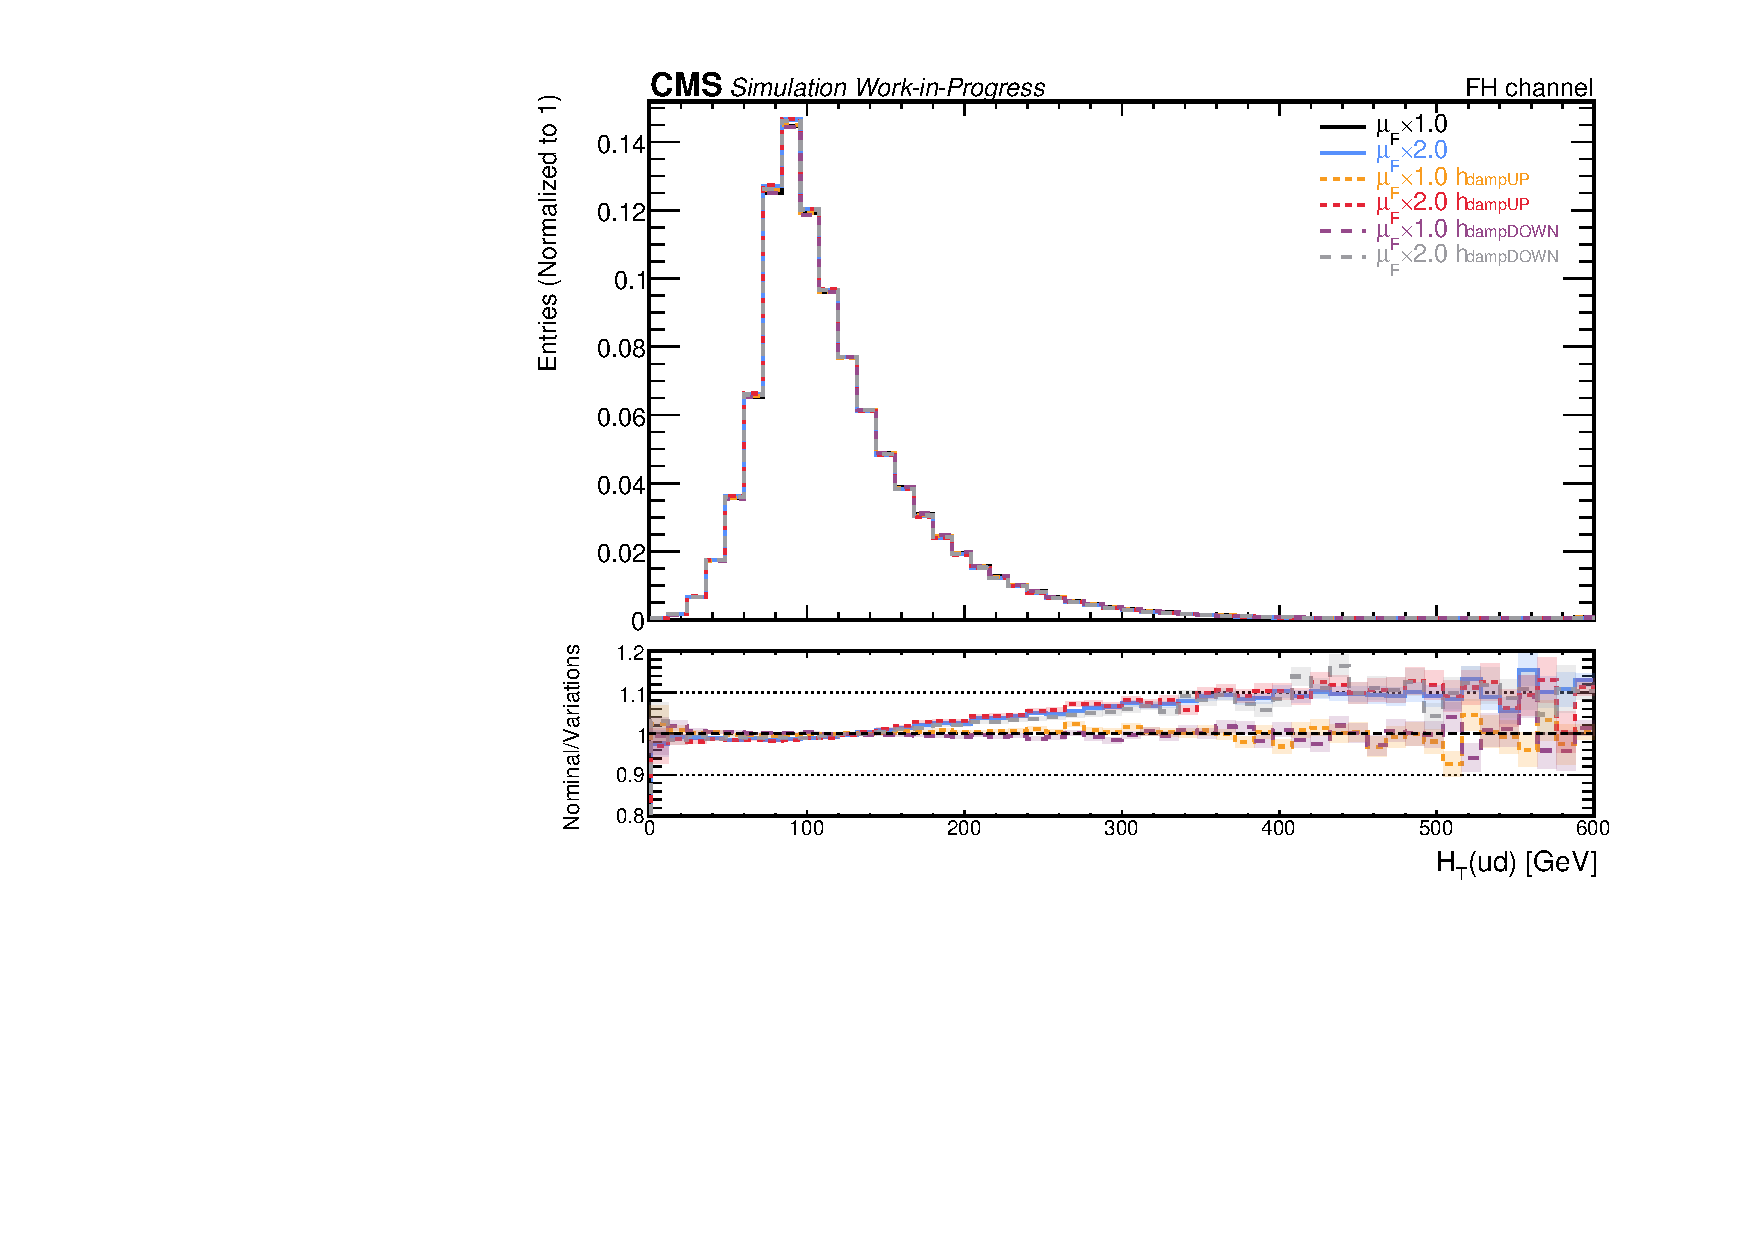
\includegraphics[width= 1.05\linewidth]{SL/ratio_ud_pairs_system_HT.pdf}
        \caption{}
        \label{subfig:HT(ud)_SL}        
    \end{subfigure}
    \hfill
    \begin{subfigure}{0.49\textwidth}
        \centering
        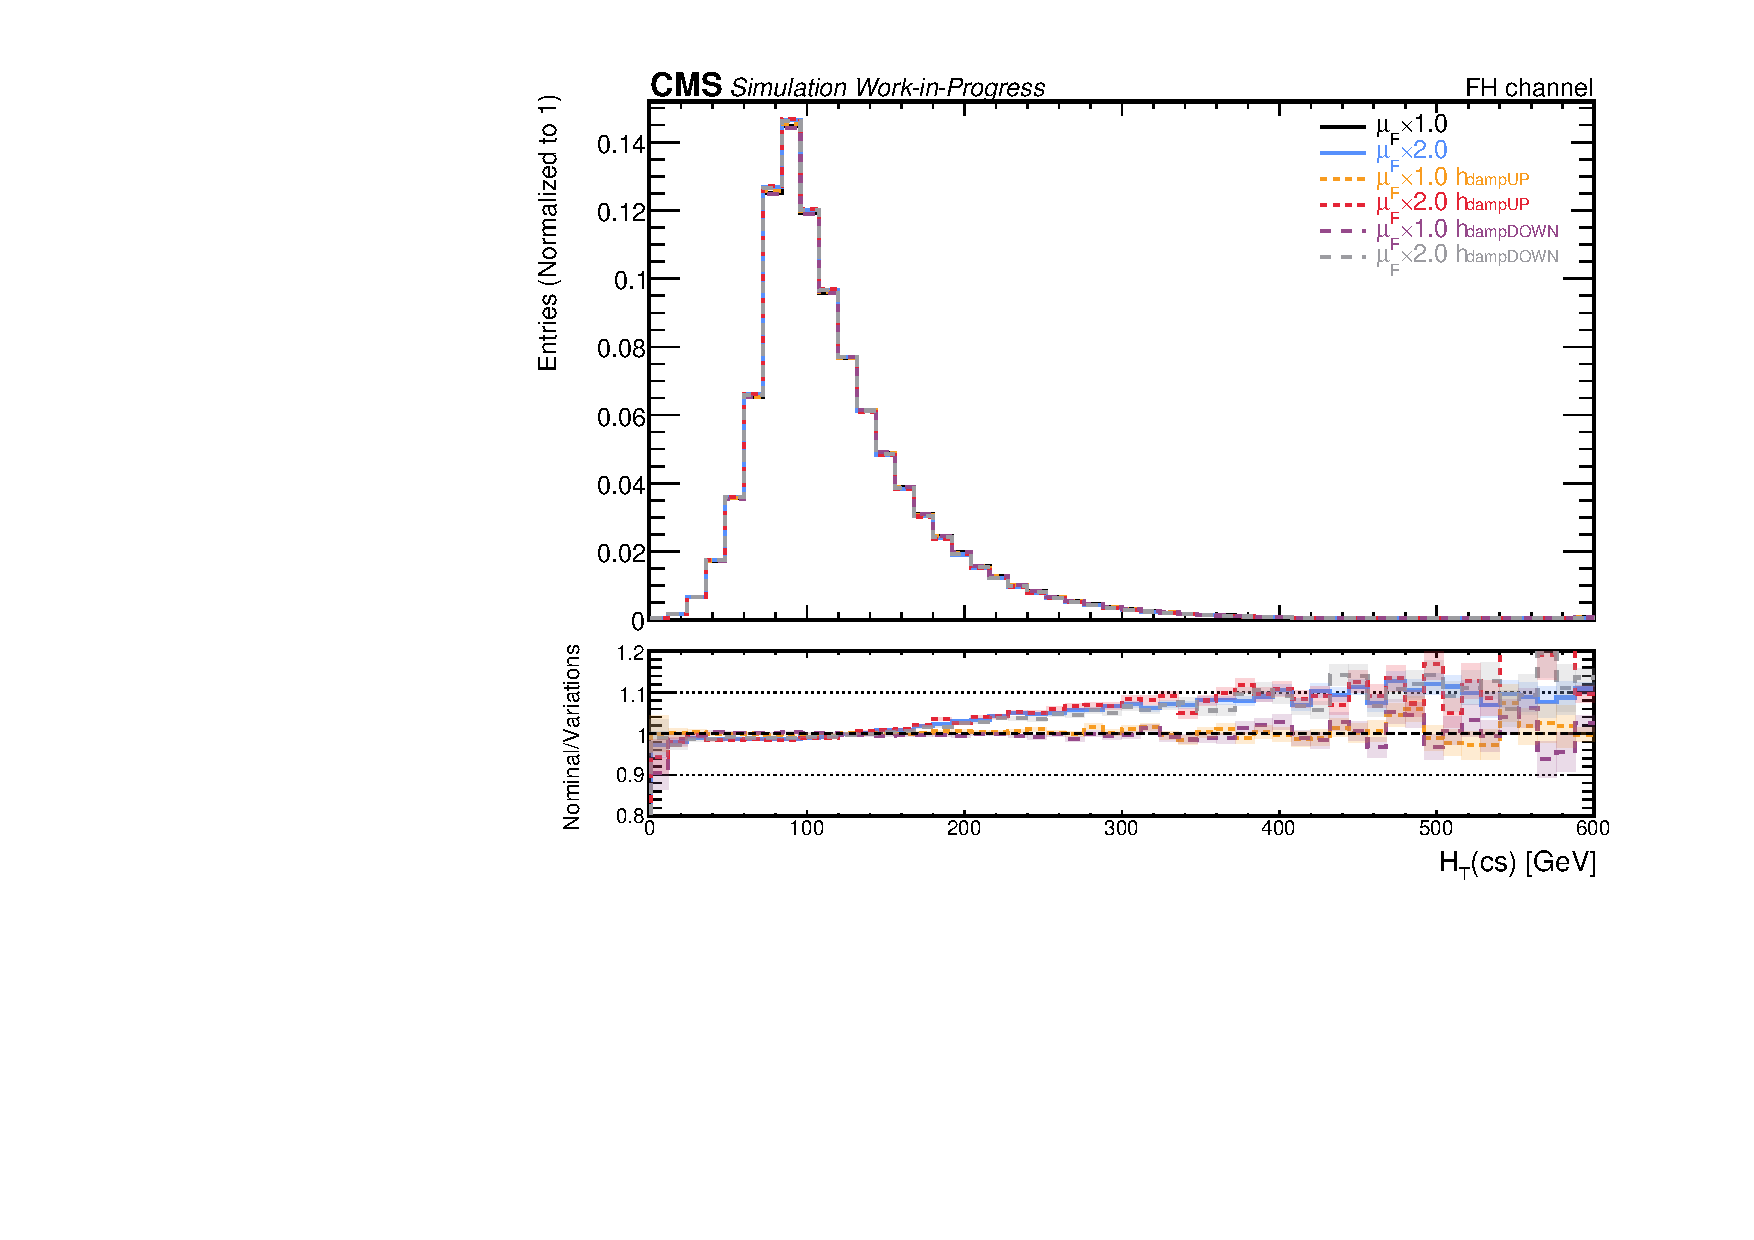
\includegraphics[width= 1.05\linewidth]{SL/ratio_sc_pairs_system_HT.pdf}
        \caption{}
        \label{subfig:HT(cs)_SL}        
    \end{subfigure}
    \hfill
        \begin{subfigure}{0.49\textwidth}
        \centering
        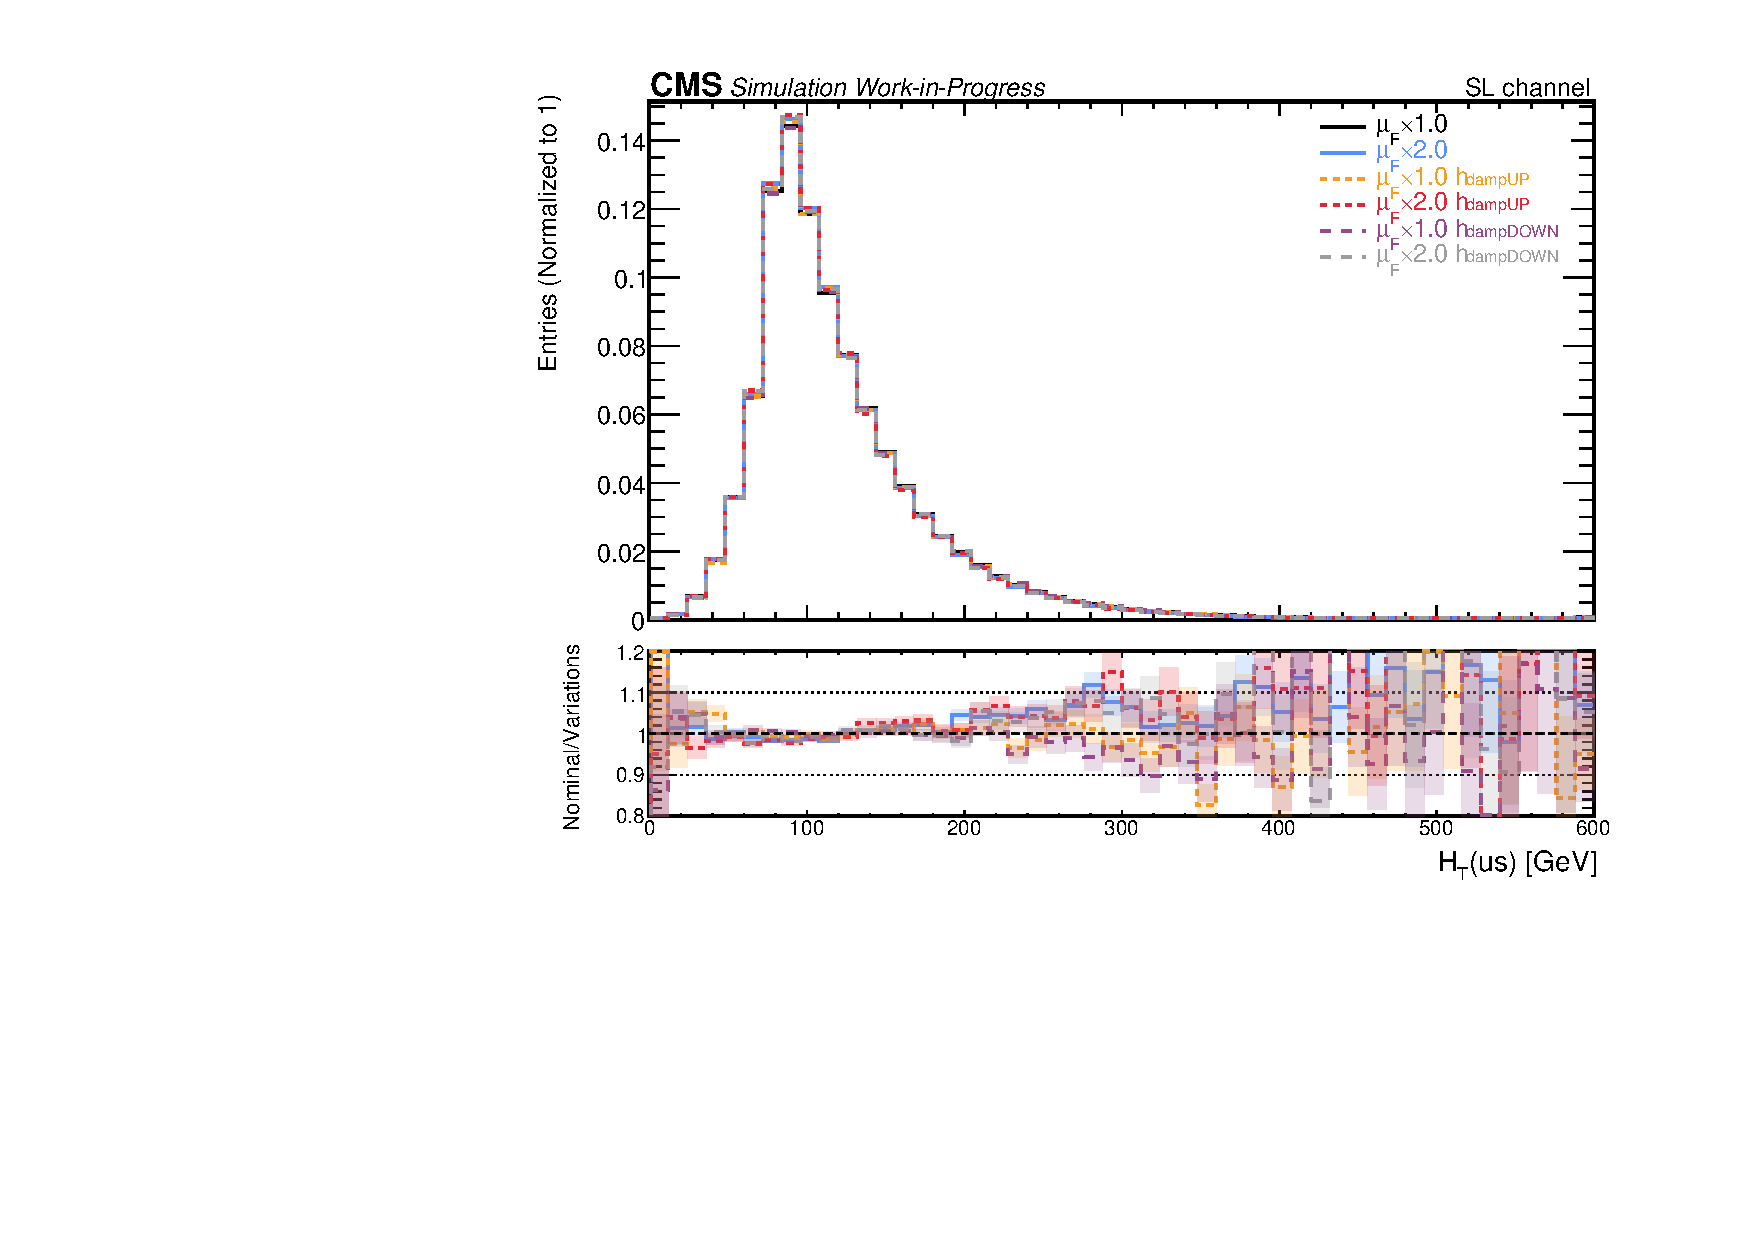
\includegraphics[width= 1.05\linewidth]{SL/ratio_su_pairs_system_HT.pdf}
        \caption{}
        \label{subfig:HT(us)_SL}        
    \end{subfigure}
    \hfill
    \begin{subfigure}{0.49\textwidth}
        \centering
        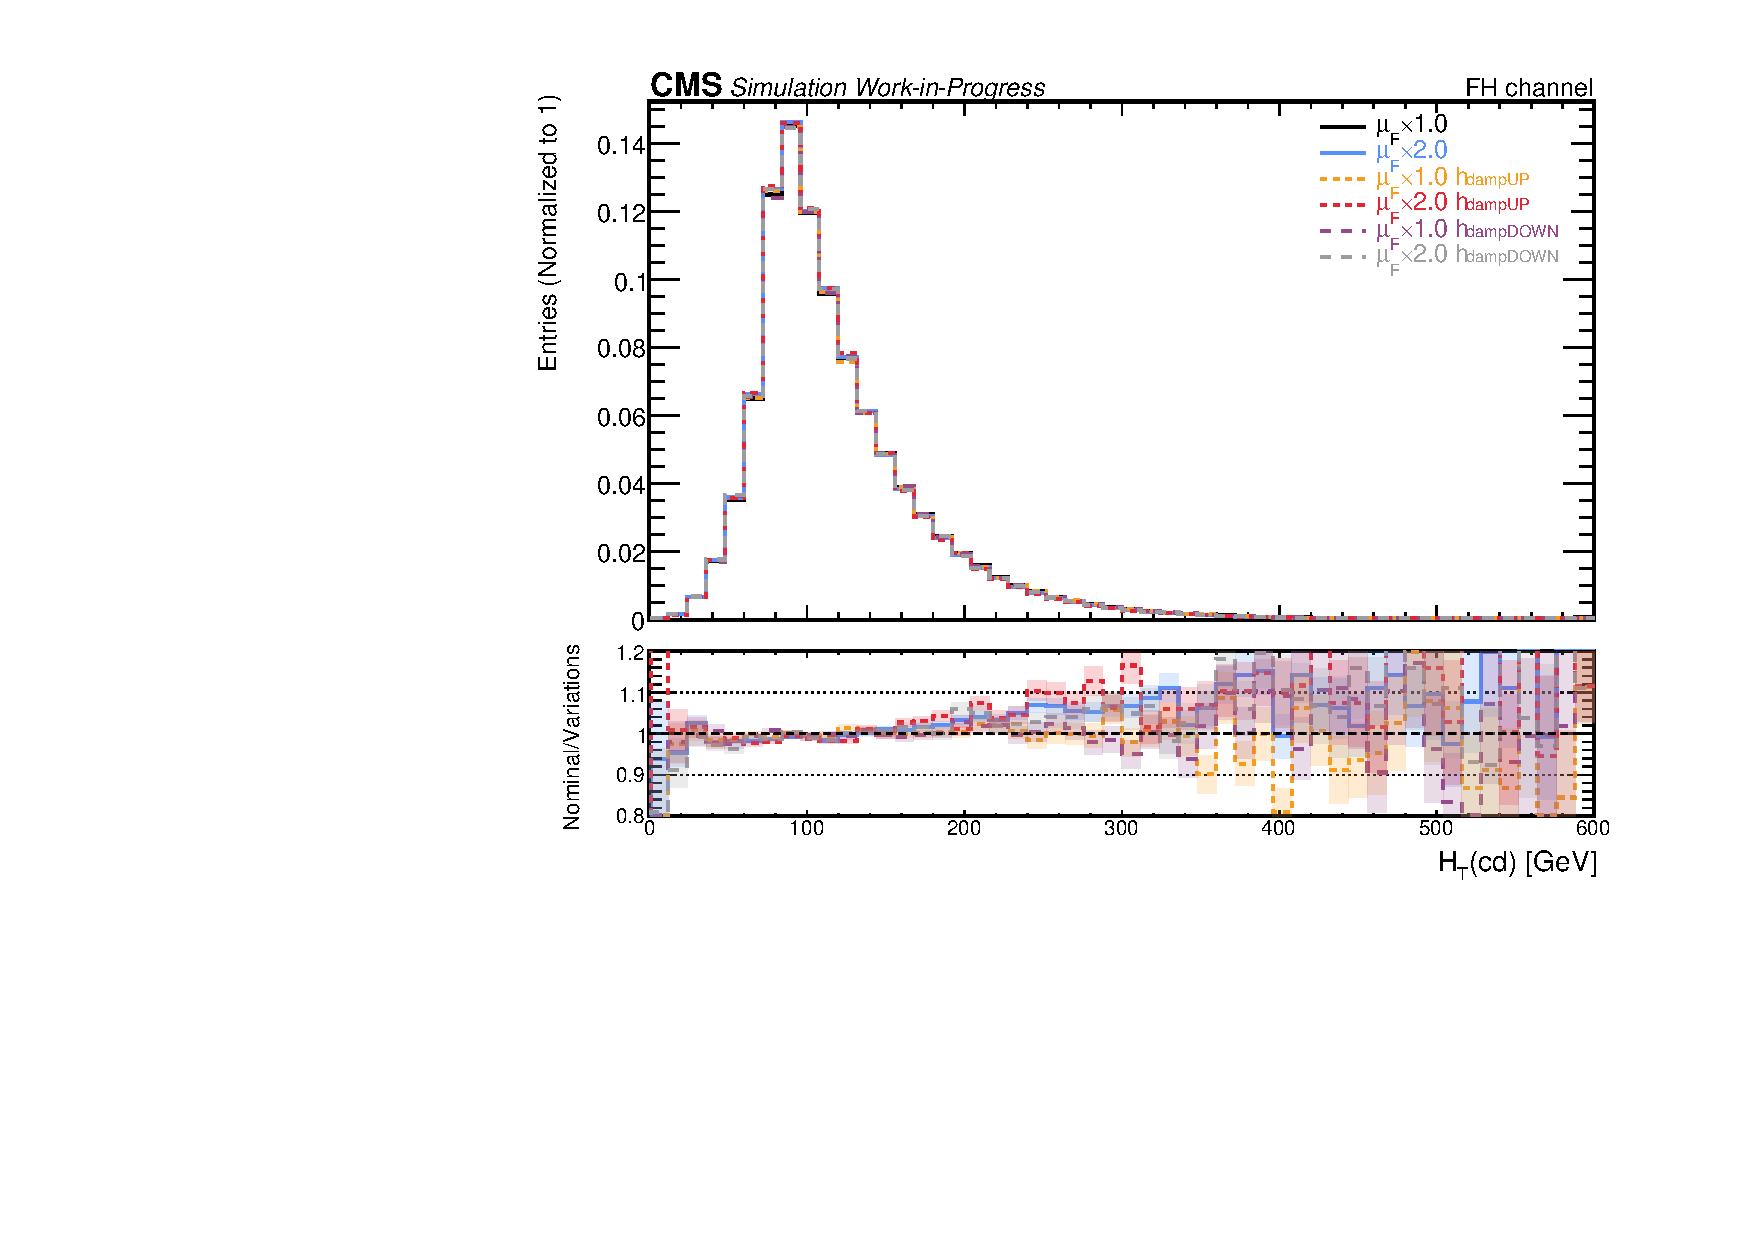
\includegraphics[width= 1.05\linewidth]{SL/ratio_cd_pairs_system_HT.pdf}
        \caption{}
        \label{subfig:HT(cd)_SL}        
    \end{subfigure}
    \caption{Distribution of H$_{\text{T}}$ for (a) ud (b) cs (c) us and (d) cd systems for the six different settings used in the simulation. The lower panel shows the ratio of the nominal setting to the variations. The shaded bands represent statistical uncertainties. The last bins contain the overflow events.}
    \label{fig:quarks_SL}
\end{figure}
\indent As for the extra light jet that is being emitted, similar to the DL channel, it is the most sensitive particle to the different h$_{\text{damp}}$ variations and in particular the hdampDOWN variation as it can be seen from Figure \ref{fig:radiation_SL}. As for the factorization scale, we observe again the same increase towards high p$_{\text{T}}$ values.
\begin{figure}[H]
    \centering
    \includegraphics[width= 0.54\linewidth]{SL/ratio_radiation_pt.pdf}
    \caption{Distribution of the transverse momentum of the extra light jet for the six different settings used in the simulation. The lower panel shows the ratio of the nominal setting to the variations. The shaded bands represent statistical uncertainties. The last bin contains the overflow events.}
    \label{fig:radiation_SL}
\end{figure}

\subsection{\label{FH}Fully hadronic channel}
\noindent For the fully hadronic channel, the final state comprises of four light flavor jets originating from the W boson decays, one extra emission of a light flavor jet from the initial particles as well as the standard four b quarks. This jet enriched final state is obviously the most difficult to model amongst the three channels.\\
\begin{figure}[H]
    \centering
    \begin{subfigure}{0.49\textwidth}
        \centering
        \includegraphics[width= 1.1\linewidth]{FH/ratio_ttbar_pt.pdf}
        \caption{}
        \label{subfig:pt(t,tbar)_FH}        
    \end{subfigure}
    \hfill
    \begin{subfigure}{0.49\linewidth}
        \centering
        \includegraphics[width= 1.1\textwidth]{FH/ratio_b_all_pt.pdf}
        \caption{}
        \label{subfig:pt(b_all)_FH}
    \end{subfigure}
    \caption{Distribution of the transverse momentum of (a) the t/$\overline{\text{t}}$ and (b) the b/$\overline{\text{b}}$ quarks for the six different settings used in the simulation. The lower panel shows the ratio of the nominal setting to the variations. The shaded bands represent statistical uncertainties. The last bins contain the overflow events.}
    \label{fig:pt_FH}
\end{figure}
\indent Naturally, as in the previous channels, here too the  interesting observables are the transverse momentum and H$_{\text{T}}$. The results for these variables for the heavy quarks in the event are presented in Figures \ref{fig:pt_FH} and \ref{fig:HT_FH}. Again, the most significant parameter change is the factorization scale. We can see that for both t/$\overline{\text{t}}$ and b/$\overline{\text{b}}$ quarks, the ratio is increasing as the transverse momentum increases. This basically, indicates that by increasing the factorization scale, the heavy quarks are generated less energetic in comparison to the nominal setting.
\begin{figure}[H]
    \centering
    \begin{subfigure}{0.49\textwidth}
        \centering
        \includegraphics[width= 1.1\linewidth]{FH/ratio_tt_system_HT.pdf}
        \caption{}
        \label{subfig:HT(ttbar)_FH}
    \end{subfigure}
    \hfill
    \begin{subfigure}{0.49\textwidth}
        \centering
        \includegraphics[width= 1.1\linewidth]{FH/ratio_prompt_bs_HT.pdf}
        \caption{}
        \label{subfig:HT(bbbar_prompt)_FH}
    \end{subfigure}
    \hfill
    \begin{subfigure}{0.49\textwidth}
        \centering
        \includegraphics[width= 1.1\linewidth]{FH/ratio_bs_from_top_HT.pdf}
        \caption{}
        \label{subfig:HT(bbbar)_FH}
    \end{subfigure}
    \caption{Distribution of H$_{\text{T}}$ for (a) t$\overline{\text{t}}$, (b) prompt b$\overline{\text{b}}$ and (c) b$\overline{\text{b}}$, originating from top quarks, systems for the six different settings used in the simulation. The lower panel shows the ratio of the nominal setting to the variations. The shaded bands represent statistical uncertainties. The last bins contain the overflow events.}
    \label{fig:HT_FH}
\end{figure}
The same can also be said for the H$_{\text{T}}$ of the particle systems, t$\overline{\text{t}}$ and the subsequent b$\overline{\text{b}}$ system from the top decays. For the t$\overline{\text{t}}$ system especially, we observe a small drop at the ratio plot in the low H$_{\text{T}}$ values that reaches up to 8 \% difference and slowly moving up, reaching the other end of the H$_{\text{T}}$ spectrum with an up to 10 \% difference, this time above the line corresponding to the nominal setting. The b$\overline{\text{b}}$ system that comes from the top quarks, exhibit the same behavior but to a lesser extent. The results for the prompt b$\overline{\text{b}}$ system are again different. This system seems to be almost unaffected by any different setting. Only a small deviation at very low H$_{\text{T}}$ values is observed for the different factorization scale settings, while the rest of the spectrum seems to be consistent with the nominal settings with only small differences of 2\%  being observed. \\
\begin{figure}[H]
    \centering
    \begin{subfigure}{0.49\textwidth}
        \centering
        \includegraphics[width= 1.1\linewidth]{FH/ratio_invariant_mass_hist.pdf}
        \caption{}
        \label{subfig:m(ttbb)_FH}        
    \end{subfigure}
    \hfill
    \begin{subfigure}{0.49\linewidth}
        \centering
        \includegraphics[width= 1.1\linewidth]{FH/ratio_Ht_hist.pdf}
        \caption{}
        \label{subfig:HT(ttbb)_FH}
    \end{subfigure}
    \caption{Distribution of (a) invariant mass and (b) H$_{\text{T}}$ for the t$\overline{\text{t}}$+b$\overline{\text{b}}$ system for the six different settings used in the simulation. The lower panel shows the ratio of the nominal setting to the variations. The shaded bands represent statistical uncertainties. The last bins contain the overflow events.}
    \label{fig:ttbb_FH}
\end{figure}
\begin{figure}[H]
    \centering
    \begin{subfigure}{0.49\textwidth}
        \centering
        \includegraphics[width= 1.1\linewidth]{FH/ratio_quarks_pt.pdf}
        \caption{}
        \label{subfig:pt(quarks)_FH}        
    \end{subfigure}
    \hfill
    \begin{subfigure}{0.49\linewidth}
        \centering
        \includegraphics[width= 1.1\linewidth]{FH/ratio_quarks_system_HT.pdf}
        \caption{}
        \label{subfig:HT(qq)_FH}
    \end{subfigure}
    \caption{Distribution of (a) the transverse momentum of all the quarks and (b) the H$_{\text{T}}$ of $\overline{\text{q}}$q' system for the six different settings used in the simulation. The lower panel shows the ratio of the nominal setting to the variations. The shaded bands represent statistical uncertainties. The last bins contain the overflow events.}
    \label{fig:quarks_all_FH}
\end{figure}
\indent Figure \ref{fig:ttbb_FH}, illustrates the distributions of the invariant mass and the H${\text{T}}$ for the t$\overline{\text{t}}$+b$\overline{\text{b}}$ system. The samples with $\mu_F \times 2$ exhibit a significant impact on both distributions, similar to what was observed in the other two channels. Regarding the various damping parameters, there is virtually no difference among them for H${\text{T}}$. However, this consistency does not hold for the invariant mass, which shows notable deviations at very high values, particularly in the hdampDOWN setting.\\
\begin{figure}[H]
    \centering
    \begin{subfigure}{0.49\textwidth}
        \centering
        \includegraphics[width= 1.1\linewidth]{FH/ratio_ud_pairs_system_HT.pdf}
        \caption{}
        \label{subfig:HT(ud)_FH}        
    \end{subfigure}
    \hfill
    \begin{subfigure}{0.49\textwidth}
        \centering
        \includegraphics[width= 1.1\linewidth]{FH/ratio_sc_pairs_system_HT.pdf}
        \caption{}
        \label{subfig:HT(cs)_FH}        
    \end{subfigure}
    \hfill
        \begin{subfigure}{0.49\textwidth}
        \centering
        \includegraphics[width= 1.1\linewidth]{FH/ratio_su_pairs_system_HT.pdf}
        \caption{}
        \label{subfig:HT(us)_FH}        
    \end{subfigure}
    \hfill
    \begin{subfigure}{0.49\textwidth}
        \centering
        \includegraphics[width= 1.1\linewidth]{FH/ratio_cd_pairs_system_HT.pdf}
        \caption{}
        \label{subfig:HT(cd)_FH}        
    \end{subfigure}
    \caption{Distribution of H$_{\text{T}}$ for (a) ud (b) cs (c) us and (d) cd systems for the six different settings used in the simulation. The lower panel shows the ratio of the nominal setting to the variations. The shaded bands represent statistical uncertainties. The last bins contain the overflow events.}
    \label{fig:quarks_FH}
\end{figure}
\indent As for the light flavor quarks, the distributions for the transverse momentum and the H$_{\text{T}}$ are illustrated in Figures \ref{subfig:pt(quarks)_FH} and \ref{subfig:HT(qq)_FH} respectively. As expected, the trend observed in these plots is similar to the heavier quarks. In particular, there is a strong deviation to the change of the factorization scale, while again, the different h$_{damp}$ variations do not affect in significant manner the distributions. As for the different quark-antiquark combinations, the distribution of their H$_{\text{T}}$ is presented in Figure \ref{fig:quarks_FH}. Similar to the SL channel, the results from the two Cabibbo suppressed pairs us (\ref{subfig:HT(us)_FH}) and cd (\ref{subfig:HT(cd)_FH}), due to low statistics have significant fluctuations, while the other two, favored quark-antiquark pairs, ud (\ref{subfig:HT(ud)_FH}) and cs (\ref{subfig:HT(cs)_FH}), obviously exhibit the same behavior with the aggregated plot.
% \begin{figure}[H]
%     \centering
%     \begin{subfigure}{0.49\textwidth}
%         \centering
%         \includegraphics[width= 1.1\linewidth]{FH/ratio_tt_system_dR.pdf}
%         \caption{}
%         \label{subfig:dR(ttbar)_FH}        
%     \end{subfigure}
%     \hfill
%     \begin{subfigure}{0.49\linewidth}
%         \centering
%         \includegraphics[width= 1.1\linewidth]{FH/ratio_prompt_bs_dR.pdf}
%         \caption{}
%         \label{subfig:dR(bbbar_prompt)_FH}
%     \end{subfigure}
%     \caption{Distribution of the angular separation of (a) t$\overline{\text{t}}$ and (b) prompt b$\overline{\text{b}}$ systems for the six different settings used in the simulation. The lower panel shows the ratio of the nominal setting to the variations. The shaded bands represent statistical uncertainties. The last bins contain the overflow events.}
%     \label{fig:dR_FH}
% \end{figure} 
\begin{figure}[H]
    \centering
    \includegraphics[width= 0.54\linewidth]{FH/ratio_radiation_pt.pdf}
    \caption{Distribution of the transverse momentum of the extra light jet for the six different settings used in the simulation. The lower panel shows the ratio of the nominal setting to the variations. The shaded bands represent statistical uncertainties. The last bins contain the overflow events.}
    \label{fig:radiation_FH}
\end{figure}
\indent Finally, for the extra radiated particle, as we can see from \ref{fig:radiation_FH}, it displays similar results to the other two channels. Specifically, for this particle's transverse momentum, there is a strong trend not only in the selection of the factorization scale but also in the hdampDOWN variation. In fact, the hdampDOWN variation with $\mu_F \times 1$, has similar deviations as the $\mu_F \times 2$. As for the hdampUP variations, again, there isn't a significant deviation from the nominal settings. 
% \begin{figure}[H]
%     \centering
%     \begin{subfigure}{0.32\textwidth}
%         \centering
%         \includegraphics[width= 1.0\linewidth]{FH/ratio_ee_system_HT.pdf}
%         \caption{}
%         \label{subfig:HT(ee)_FH}
%     \end{subfigure}
% \hfill
%     \begin{subfigure}{0.32\textwidth}
%         \centering
%         \includegraphics[width= 1.0\linewidth]{FH/ratio_mm_system_HT.pdf}
%         \caption{}
%         \label{subfig:HT(mm)_FH}
%     \end{subfigure}
% \hfill
%     \begin{subfigure}{0.32\textwidth}
%         \centering
%         \includegraphics[width= 1.0\linewidth]{FH/ratio_tautau_system_HT.pdf}
%         \caption{}
%         \label{subfig:HT(tt)_FH}
%     \end{subfigure}

%     \vspace{0.2cm}

%     \begin{subfigure}{0.32\textwidth}
%         \centering
%         \includegraphics[width= 1.0\linewidth]{FH/ratio_em_system_HT.pdf}
%         \caption{}
%         \label{subfig:HT(em)_FH}
%     \end{subfigure}
% \hfill
%     \begin{subfigure}{0.32\textwidth}
%         \centering
%         \includegraphics[width= 1.0\linewidth]{FH/ratio_et_system_HT.pdf}
%         \caption{}
%         \label{subfig:HT(et)_FH}
%     \end{subfigure}
% \hfill
%     \begin{subfigure}{0.32\textwidth}
%         \centering
%         \includegraphics[width= 1.0\linewidth]{FH/ratio_mt_system_HT.pdf}
%         \caption{}
%         \label{subfig:HT(mt)_FH}
%     \end{subfigure}
%     \caption{Distribution of H$_\text{T}$ for (a) $e^-e^+$, (b) $\mu^-\mu^+$, (c) $\tau^-\tau^+$, (d) $e\mu$ (e) $e\tau$ and (f) $\mu\tau$ systems for the six different settings used in the simulation. The lower panel shows the ratio of the nominal setting to the variations. The shaded bands represent statistical uncertainties. }
%     \label{fig:HT(ll_all)_FH}
% \end{figure}


















% \begin{figure}[H]
%     \centering
%     \begin{subfigure}{0.7\textwidth}
%         \centering
%         \includegraphics[width= 1.0\linewidth]{DL/ratio_tt_system_HT.pdf}
%         \caption{}
%         \label{subfig:HT(ttbar)_DL}
%     \end{subfigure}
    
%     \vspace{0.2cm}
        
%     \begin{subfigure}{0.7\textwidth}
%         \centering
%         \includegraphics[width= 1.0\linewidth]{DL/ratio_tt_system_dR.pdf}
%         \caption{}
%         \label{subfig:dR(ttbar)_DL}
%     \end{subfigure}
    
%     \caption{Distributions of (a) H$_{\text{T}}$ and (b) angular separation of the t$\overline{\text{t}}$ system for the six different settings used in the simulation. The lower panel shows the ratio of the nominal setting to the variations. The shaded bands represent statistical uncertainties. The last bins contain the overflow events.}
%     \label{fig:ttbar_DL}
% \end{figure}


% \begin{figure}[H]
%     \centering
%     \includegraphics[width= 1.0\linewidth]{DL/ratio_b_all_pt.pdf}
%     \caption{Distribution of the transverse momentum of all the b/$\overline{\text{b}}$ quarks for the six different settings used in the simulation. The lower panel shows the ratio of the nominal setting to the variations. The shaded bands represent statistical uncertainties. The last bins contain the overflow events.}
%     \label{fig:b_all_DL}
% \end{figure}

% \begin{figure}[H]
%     \centering
%     \begin{subfigure}{0.7\textwidth}
%         \centering
%         \includegraphics[width= 1.0\linewidth]{DL/ratio_bs_from_top_HT.pdf}
%         \caption{}
%         \label{subfig:HT(bbbar)_DL}
%     \end{subfigure}
    
%     \vspace{0.2cm}
        
%     \begin{subfigure}{0.7\textwidth}
%         \centering
%         \includegraphics[width= 1.0\linewidth]{DL/ratio_bs_from_top_dR.pdf}
%         \caption{}
%         \label{subfig:dR(bbbar)_DL}
%     \end{subfigure}
    
%     \caption{Distributions of (a) H$_{\text{T}}$ and (b) angular separation of the b$\overline{\text{b}}$ system, related to top quarks, for the six different settings used in the simulation. The lower panel shows the ratio of the nominal setting to the variations. The shaded bands represent statistical uncertainties. The last bins contain the overflow events.}
%     \label{fig:ttbar_DL}
% \end{figure}


% \begin{figure}[H]
%     \centering
%     \begin{subfigure}{0.7\textwidth}
%         \centering
%         \includegraphics[width= 1.0\linewidth]{DL/ratio_prompt_bs_HT.pdf}
%         \caption{}
%         \label{subfig:HT(bbbar_prompt)_DL}
%     \end{subfigure}
    
%     \vspace{0.2cm}
        
%     \begin{subfigure}{0.7\textwidth}
%         \centering
%         \includegraphics[width= 1.0\linewidth]{DL/ratio_prompt_bs_dR.pdf}
%         \caption{}
%         \label{subfig:dR(bbbar_prompt)_DL}
%     \end{subfigure}
    
%     \caption{Distributions of (a) H$_{\text{T}}$ and (b) angular separation of the prompt b$\overline{\text{b}}$ system for the six different settings used in the simulation. The lower panel shows the ratio of the nominal setting to the variations. The shaded bands represent statistical uncertainties. The last bins contain the overflow events.}
%     \label{fig:ttbar_DL}
% \end{figure}


% \begin{figure}[H]
%     \centering
%     \includegraphics[width= 0.7\linewidth]{DL/ratio_leptons_pt.pdf}
%     \caption{Distribution of the transverse momentum of all the leptons (charged or neutral) for the six different settings used in the simulation. The lower panel shows the ratio of the nominal setting to the variations. The shaded bands represent statistical uncertainties. The last bins contain the overflow events.}
%     \label{fig:leptons_DL}
% \end{figure}



% \begin{figure}[H]
%     \centering
%     \begin{subfigure}{0.7\textwidth}
%         \centering
%         \includegraphics[width= 1.0\linewidth]{DL/ratio_ll_system_HT.pdf}
%         \caption{}
%         \label{subfig:HT(ll)_DL}
%     \end{subfigure}
    
% \hfill
        
%     \begin{subfigure}{0.7\textwidth}
%         \centering
%         \includegraphics[width= 1.0\linewidth]{DL/ratio_ll_system_dR.pdf}
%         \caption{}
%         \label{subfig:dR(ll)_DL}
%     \end{subfigure}
    
%     \caption{Distributions of (a) H$_{\text{T}}$ and (b) angular separation of the $\ell^-\ell^+$ system for the six different settings used in the simulation. The lower panel shows the ratio of the nominal setting to the variations. The shaded bands represent statistical uncertainties. The last bins contain the overflow events.}
%     \label{fig:ttbar_DL}
% \end{figure}






% \begin{figure}[H]
%     \centering
%     \includegraphics[width= 1.0\linewidth]{DL/ratio_radiation_pt.pdf}
%     \caption{Distribution of the transverse momentum of the extra light jet for the six different settings used in the simulation. The lower panel shows the ratio of the nominal setting to the variations. The shaded bands represent statistical uncertainties. The last bins contain the overflow events.}
%     \label{fig:radiation_DL}
% \end{figure}


% %================================================================


% 

% \begin{figure}[H]
%     \centering
%     \begin{subfigure}{0.7\textwidth}
%         \centering
%         \includegraphics[width= 1.0\linewidth]{SL/ratio_ttbar_pt.pdf}
%         \caption{}
%         \label{subfig:pt(t,tbar)_SL}
%     \end{subfigure}

%     \vspace{0.2cm}
    
%     \begin{subfigure}{0.7\textwidth}
%         \centering
%         \includegraphics[width= 1.0\linewidth]{SL/ratio_ttbar_reco_mass.pdf}
%         \caption{}
%         \label{subfig:m(t,tbar)_SL}
%     \end{subfigure}
    
%     \caption{Distributions of (a) transverse momentum and (b) reconstructed mass of the t/$\overline{\text{t}}$ quarks for the six different settings used in the simulation. The lower panel shows the ratio of the nominal setting to the variations. The shaded bands represent statistical uncertainties. The last bins contain the overflow events.}
%     \label{fig:t,tbar_SL}
% \end{figure}



% \begin{figure}[H]
%     \centering
%     \begin{subfigure}{0.7\textwidth}
%         \centering
%         \includegraphics[width= 1.0\linewidth]{SL/ratio_tt_system_HT.pdf}
%         \caption{}
%         \label{subfig:HT(ttbar)_SL}
%     \end{subfigure}
    
%     \vspace{0.2cm}
        
%     \begin{subfigure}{0.7\textwidth}
%         \centering
%         \includegraphics[width= 1.0\linewidth]{SL/ratio_tt_system_dR.pdf}
%         \caption{}
%         \label{subfig:dR(ttbar)_SL}
%     \end{subfigure}
    
%     \caption{Distributions of (a) H$_{\text{T}}$ and (b) angular separation of the t$\overline{\text{t}}$ system for the six different settings used in the simulation. The lower panel shows the ratio of the nominal setting to the variations. The shaded bands represent statistical uncertainties. The last bins contain the overflow events.}
%     \label{fig:ttbar_SL}
% \end{figure}


% \begin{figure}[H]
%     \centering
%     \includegraphics[width= 1.0\linewidth]{SL/ratio_b_all_pt.pdf}
%     \caption{Distribution of the transverse momentum of all the b/$\overline{\text{b}}$ quarks for the six different settings used in the simulation. The lower panel shows the ratio of the nominal setting to the variations. The shaded bands represent statistical uncertainties. The last bins contain the overflow events.}
%     \label{fig:b_all_SL}
% \end{figure}

% \begin{figure}[H]
%     \centering
%     \begin{subfigure}{0.7\textwidth}
%         \centering
%         \includegraphics[width= 1.0\linewidth]{SL/ratio_bs_from_top_HT.pdf}
%         \caption{}
%         \label{subfig:HT(bbbar)_SL}
%     \end{subfigure}
    
%     \vspace{0.2cm}
        
%     \begin{subfigure}{0.7\textwidth}
%         \centering
%         \includegraphics[width= 1.0\linewidth]{SL/ratio_bs_from_top_dR.pdf}
%         \caption{}
%         \label{subfig:dR(bbbar)_SL}
%     \end{subfigure}
    
%     \caption{Distributions of (a) H$_{\text{T}}$ and (b) angular separation of the b$\overline{\text{b}}$ system, related to top quarks, for the six different settings used in the simulation. The lower panel shows the ratio of the nominal setting to the variations. The shaded bands represent statistical uncertainties. The last bins contain the overflow events.}
%     \label{fig:ttbar_SL}
% \end{figure}


% \begin{figure}[H]
%     \centering
%     \begin{subfigure}{0.7\textwidth}
%         \centering
%         \includegraphics[width= 1.0\linewidth]{SL/ratio_prompt_bs_HT.pdf}
%         \caption{}
%         \label{subfig:HT(bbbar_prompt)_SL}
%     \end{subfigure}
    
%     \vspace{0.2cm}
        
%     \begin{subfigure}{0.7\textwidth}
%         \centering
%         \includegraphics[width= 1.0\linewidth]{SL/ratio_prompt_bs_dR.pdf}
%         \caption{}
%         \label{subfig:dR(bbbar_prompt)_SL}
%     \end{subfigure}
    
%     \caption{Distributions of (a) H$_{\text{T}}$ and (b) angular separation of the prompt b$\overline{\text{b}}$ system for the six different settings used in the simulation. The lower panel shows the ratio of the nominal setting to the variations. The shaded bands represent statistical uncertainties. The last bins contain the overflow events.}
%     \label{fig:ttbar_SL}
% \end{figure}


% \begin{figure}[H]
%     \centering
%     \includegraphics[width= 0.7\linewidth]{SL/ratio_leptons_pt.pdf}
%     \caption{Distribution of the transverse momentum of all the leptons (charged or neutral) for the six different settings used in the simulation. The lower panel shows the ratio of the nominal setting to the variations. The shaded bands represent statistical uncertainties. The last bins contain the overflow events.}
%     \label{fig:leptons_SL}
% \end{figure}




% \begin{figure}[H]
%     \centering
%     \includegraphics[width= 1.0\linewidth]{SL/ratio_radiation_pt.pdf}
%     \caption{Distribution of the transverse momentum of the extra light jet for the six different settings used in the simulation. The lower panel shows the ratio of the nominal setting to the variations. The shaded bands represent statistical uncertainties. The last bins contain the overflow events.}
%     \label{fig:radiation_SL}
% \end{figure}







% \subsection{\label{FH}Fully hadronic channel}


% \begin{figure}[H]
%     \centering
%     \begin{subfigure}{0.7\textwidth}
%         \centering
%         \includegraphics[width= 1.0\linewidth]{FH/ratio_ttbar_pt.pdf}
%         \caption{}
%         \label{subfig:pt(t,tbar)_FH}
%     \end{subfigure}

%     \vspace{0.2cm}
    
%     \begin{subfigure}{0.7\textwidth}
%         \centering
%         \includegraphics[width= 1.0\linewidth]{FH/ratio_ttbar_reco_mass.pdf}
%         \caption{}
%         \label{subfig:m(t,tbar)_FH}
%     \end{subfigure}
    
%     \caption{Distributions of (a) transverse momentum and (b) reconstructed mass of the t/$\overline{\text{t}}$ quarks for the six different settings used in the simulation. The lower panel shows the ratio of the nominal setting to the variations. The shaded bands represent statistical uncertainties. The last bins contain the overflow events.}
%     \label{fig:t,tbar_FH}
% \end{figure}



% \begin{figure}[H]
%     \centering
%     \begin{subfigure}{0.7\textwidth}
%         \centering
%         \includegraphics[width= 1.0\linewidth]{FH/ratio_tt_system_HT.pdf}
%         \caption{}
%         \label{subfig:HT(ttbar)_FH}
%     \end{subfigure}
    
%     \vspace{0.2cm}
        
%     \begin{subfigure}{0.7\textwidth}
%         \centering
%         \includegraphics[width= 1.0\linewidth]{FH/ratio_tt_system_dR.pdf}
%         \caption{}
%         \label{subfig:dR(ttbar)_FH}
%     \end{subfigure}
    
%     \caption{Distributions of (a) H$_{\text{T}}$ and (b) angular separation of the t$\overline{\text{t}}$ system for the six different settings used in the simulation. The lower panel shows the ratio of the nominal setting to the variations. The shaded bands represent statistical uncertainties. The last bins contain the overflow events.}
%     \label{fig:ttbar_FH}
% \end{figure}


% \begin{figure}[H]
%     \centering
%     \includegraphics[width= 1.0\linewidth]{FH/ratio_b_all_pt.pdf}
%     \caption{Distribution of the transverse momentum of all the b/$\overline{\text{b}}$ quarks for the six different settings used in the simulation. The lower panel shows the ratio of the nominal setting to the variations. The shaded bands represent statistical uncertainties. The last bins contain the overflow events.}
%     \label{fig:b_all_FH}
% \end{figure}

% \begin{figure}[H]
%     \centering
%     \begin{subfigure}{0.7\textwidth}
%         \centering
%         \includegraphics[width= 1.0\linewidth]{FH/ratio_bs_from_top_HT.pdf}
%         \caption{}
%         \label{subfig:HT(bbbar)_FH}
%     \end{subfigure}
    
%     \vspace{0.2cm}
        
%     \begin{subfigure}{0.7\textwidth}
%         \centering
%         \includegraphics[width= 1.0\linewidth]{FH/ratio_bs_from_top_dR.pdf}
%         \caption{}
%         \label{subfig:dR(bbbar)_FH}
%     \end{subfigure}
    
%     \caption{Distributions of (a) H$_{\text{T}}$ and (b) angular separation of the b$\overline{\text{b}}$ system, related to top quarks, for the six different settings used in the simulation. The lower panel shows the ratio of the nominal setting to the variations. The shaded bands represent statistical uncertainties. The last bins contain the overflow events.}
%     \label{fig:ttbar_FH}
% \end{figure}


% \begin{figure}[H]
%     \centering
%     \begin{subfigure}{0.7\textwidth}
%         \centering
%         \includegraphics[width= 1.0\linewidth]{FH/ratio_prompt_bs_HT.pdf}
%         \caption{}
%         \label{subfig:HT(bbbar_prompt)_FH}
%     \end{subfigure}
    
%     \vspace{0.2cm}
        
%     \begin{subfigure}{0.7\textwidth}
%         \centering
%         \includegraphics[width= 1.0\linewidth]{FH/ratio_prompt_bs_dR.pdf}
%         \caption{}
%         \label{subfig:dR(bbbar_prompt)_FH}
%     \end{subfigure}
    
%     \caption{Distributions of (a) H$_{\text{T}}$ and (b) angular separation of the prompt b$\overline{\text{b}}$ system for the six different settings used in the simulation. The lower panel shows the ratio of the nominal setting to the variations. The shaded bands represent statistical uncertainties. The last bins contain the overflow events.}
%     \label{fig:ttbar_FH}
% \end{figure}


% \begin{figure}[H]
%     \centering
%     \includegraphics[width= 1.0\linewidth]{FH/ratio_radiation_pt.pdf}
%     \caption{Distribution of the transverse momentum of the extra light jet for the six different settings used in the simulation. The lower panel shows the ratio of the nominal setting to the variations. The shaded bands represent statistical uncertainties. The last bins contain the overflow events.}
%     \label{fig:radiation_FH}
% \end{figure}








% %===========================================================================================================

% %--------------quarks

% \begin{figure}[H]
%     \centering
%     \begin{subfigure}{0.49\textwidth}
%         \centering
%         \includegraphics[width= 1.0\linewidth]{FH/ratio_quarks_energy.pdf}
%         \caption{}
%         \label{subfig:E(quarks)_FH}
%     \end{subfigure}
%     \begin{subfigure}{0.49\textwidth}
%         \centering
%         \includegraphics[width= 1.0\linewidth]{FH/ratio_quarks_pt.pdf}
%         \caption{}
%         \label{subfig:pt(quarks)_FH}
%     \end{subfigure}

%     \vspace{0.2cm}
    
%     \begin{subfigure}{0.49\textwidth}
%         \centering
%         \includegraphics[width= 1.0\linewidth]{FH/ratio_quarks_phi.pdf}
%         \caption{}
%         \label{subfig:phi(quarks)_FH}
%     \end{subfigure}
%     \begin{subfigure}{0.49\textwidth}
%         \centering
%         \includegraphics[width= 1.0\linewidth]{FH/ratio_quarks_pseudorapidity.pdf}
%         \caption{}
%         \label{subfig:eta(quarks)_FH}
%     \end{subfigure}
%     \caption{Distributions of (a) energy, (b) transverse momentum,  (c) azimuthial angle and (d) pseudorapidity of the light flavor quarks, related to W bosons, for the six different settings used in the simulation. The lower panel shows the ratio of the nominal setting to the variations. The shaded bands represent statistical uncertainties. The last bins contain the overflow events.}
%     \label{fig:quarks_FH}
% \end{figure}


% \begin{figure}[H]
%     \centering
%     \begin{subfigure}{0.49\textwidth}
%         \centering
%         \includegraphics[width= 1.0\linewidth]{FH/ratio_quarks_system_HT.pdf}
%         \caption{}
%         \label{subfig:HT(qq)_FH}
%     \end{subfigure}
%     \begin{subfigure}{0.49\textwidth}
%         \centering
%         \includegraphics[width= 1.0\linewidth]{FH/ratio_quarks_system_invariant_mass.pdf}
%         \caption{}
%         \label{subfig:m(qq)_FH}
%     \end{subfigure}

%     \vspace{0.2cm}
    
%     \begin{subfigure}{0.49\textwidth}
%         \centering
%         \includegraphics[width= 1.0\linewidth]{FH/ratio_quarks_system_dR.pdf}
%         \caption{}
%         \label{subfig:dR(qq)_FH}
%     \end{subfigure}
%     \begin{subfigure}{0.49\textwidth}
%         \centering
%         \includegraphics[width= 1.0\linewidth]{FH/ratio_quarks_system_pseudorapidity.pdf}
%         \caption{}
%         \label{subfig:y(qq)_FH}
%     \end{subfigure}
%     \caption{Distributions of (a) H$_\text{T}$, (b) invariant mass,  (c) angular separation and (d) rapidity of the q'$\overline{\text{q}}$ system for the six different settings used in the simulation. The lower panel shows the ratio of the nominal setting to the variations. The shaded bands represent statistical uncertainties. The last bins contain the overflow events.}
%     \label{fig:qqbar_FH}
% \end{figure}



% \begin{figure}[H]
%     \centering
%     \begin{subfigure}{0.49\textwidth}
%         \centering
%         \includegraphics[width= 1.0\linewidth]{FH/ratio_ud_pairs_system_HT.pdf}
%         \caption{}
%         \label{subfig:HT(ud)_FH}
%     \end{subfigure}
%     \begin{subfigure}{0.49\textwidth}
%         \centering
%         \includegraphics[width= 1.0\linewidth]{FH/ratio_ud_pairs_system_invariant_mass.pdf}
%         \caption{}
%         \label{subfig:m(udqq)_FH}
%     \end{subfigure}

%     \vspace{0.2cm}
    
%     \begin{subfigure}{0.49\textwidth}
%         \centering
%         \includegraphics[width= 1.0\linewidth]{FH/ratio_ud_pairs_system_dR.pdf}
%         \caption{}
%         \label{subfig:dR(udqq)_FH}
%     \end{subfigure}
%     \begin{subfigure}{0.49\textwidth}
%         \centering
%         \includegraphics[width= 1.0\linewidth]{FH/ratio_ud_pairs_system_pseudorapidity.pdf}
%         \caption{}
%         \label{subfig:y(udqq)_FH}
%     \end{subfigure}
%     \caption{Distributions of (a) H$_\text{T}$, (b) invariant mass,  (c) angular separation and (d) rapidity of the ud (u$\overline{\text{d}}$+$\overline{\text{u}}$d) system for the six different settings used in the simulation. The lower panel shows the ratio of the nominal setting to the variations. The shaded bands represent statistical uncertainties. The last bins contain the overflow events.}
%     \label{fig:udqqbar_FH}
% \end{figure}

% \begin{figure}[H]
%     \centering
%     \begin{subfigure}{0.49\textwidth}
%         \centering
%         \includegraphics[width= 1.0\linewidth]{FH/ratio_sc_pairs_system_HT.pdf}
%         \caption{}
%         \label{subfig:HT(sc)_FH}
%     \end{subfigure}
%     \begin{subfigure}{0.49\textwidth}
%         \centering
%         \includegraphics[width= 1.0\linewidth]{FH/ratio_sc_pairs_system_invariant_mass.pdf}
%         \caption{}
%         \label{subfig:m(sc)_FH}
%     \end{subfigure}

%     \vspace{0.2cm}
    
%     \begin{subfigure}{0.49\textwidth}
%         \centering
%         \includegraphics[width= 1.0\linewidth]{FH/ratio_sc_pairs_system_dR.pdf}
%         \caption{}
%         \label{subfig:dR(sc)_FH}
%     \end{subfigure}
%     \begin{subfigure}{0.49\textwidth}
%         \centering
%         \includegraphics[width= 1.0\linewidth]{FH/ratio_sc_pairs_system_pseudorapidity.pdf}
%         \caption{}
%         \label{subfig:y(sc)_FH}
%     \end{subfigure}
%     \caption{Distributions of (a) H$_\text{T}$, (b) invariant mass,  (c) angular separation and (d) rapidity of the cs (c$\overline{\text{s}}$+$\overline{\text{c}}$s) system for the six different settings used in the simulation. The lower panel shows the ratio of the nominal setting to the variations. The shaded bands represent statistical uncertainties. The last bins contain the overflow events.}
%     \label{fig:sc_FH}
% \end{figure}

% \begin{figure}[H]
%     \centering
%     \begin{subfigure}{0.49\textwidth}
%         \centering
%         \includegraphics[width= 1.0\linewidth]{FH/ratio_su_pairs_system_HT.pdf}
%         \caption{}
%         \label{subfig:HT(su)_FH}
%     \end{subfigure}
%     \begin{subfigure}{0.49\textwidth}
%         \centering
%         \includegraphics[width= 1.0\linewidth]{FH/ratio_su_pairs_system_invariant_mass.pdf}
%         \caption{}
%         \label{subfig:m(su)_FH}
%     \end{subfigure}

%     \vspace{0.2cm}
    
%     \begin{subfigure}{0.49\textwidth}
%         \centering
%         \includegraphics[width= 1.0\linewidth]{FH/ratio_su_pairs_system_dR.pdf}
%         \caption{}
%         \label{subfig:dR(su)_FH}
%     \end{subfigure}
%     \begin{subfigure}{0.49\textwidth}
%         \centering
%         \includegraphics[width= 1.0\linewidth]{FH/ratio_su_pairs_system_pseudorapidity.pdf}
%         \caption{}
%         \label{subfig:y(su)_FH}
%     \end{subfigure}
%     \caption{Distributions of (a) H$_\text{T}$, (b) invariant mass,  (c) angular separation and (d) rapidity of the us (u$\overline{\text{s}}$+$\overline{\text{u}}$s) system for the six different settings used in the simulation. The lower panel shows the ratio of the nominal setting to the variations. The shaded bands represent statistical uncertainties. The last bins contain the overflow events.}
%     \label{fig:su_FH}
% \end{figure}

% \begin{figure}[H]
%     \centering
%     \begin{subfigure}{0.49\textwidth}
%         \centering
%         \includegraphics[width= 1.0\linewidth]{FH/ratio_cd_pairs_system_HT.pdf}
%         \caption{}
%         \label{subfig:HT(cd)_FH}
%     \end{subfigure}
%     \begin{subfigure}{0.49\textwidth}
%         \centering
%         \includegraphics[width= 1.0\linewidth]{FH/ratio_cd_pairs_system_invariant_mass.pdf}
%         \caption{}
%         \label{subfig:m(cd)_FH}
%     \end{subfigure}

%     \vspace{0.2cm}
    
%     \begin{subfigure}{0.49\textwidth}
%         \centering
%         \includegraphics[width= 1.0\linewidth]{FH/ratio_cd_pairs_system_dR.pdf}
%         \caption{}
%         \label{subfig:dR(cd)_FH}
%     \end{subfigure}
%     \begin{subfigure}{0.49\textwidth}
%         \centering
%         \includegraphics[width= 1.0\linewidth]{FH/ratio_cd_pairs_system_pseudorapidity.pdf}
%         \caption{}
%         \label{subfig:y(cd)_FH}
%     \end{subfigure}
%     \caption{Distributions of (a) H$_\text{T}$, (b) invariant mass,  (c) angular separation and (d) rapidity of the cs (c$\overline{\text{d}}$+$\overline{\text{c}}$d) system for the six different settings used in the simulation. The lower panel shows the ratio of the nominal setting to the variations. The shaded bands represent statistical uncertainties. The last bins contain the overflow events.}
%     \label{fig:cd_FH}
% \end{figure}

\section{Summary}
\noindent The objective of this thesis was to optimize the simulation of t$\overline{\text{t}}+$b$\overline{\text{b}}$ production, which as we saw, is a critical background in numerous experimental searches such as the t$\overline{\text{t}}$H(b$\overline{\text{b}}/$c$\overline{\text{c}}$). In particular, the sensitivity of events on the MC generator free parameter h$_{\text{damp}}$, and the factorisation scale was studied. Several sets of samples were generated with different settings using the {\fontfamily{bch}\fontshape{sc}\selectfont{Powheg Box Res}} package, for all three decay channels. The results presented in the previous sections show that different h$_{\text{damp}}$ choices have very small deviations. On the other hand, the increase of the factorization scale by a factor of two impacts the distribution of the p$_{\text{T}}$-dependent variables significantly.\\
% 
\indent Throughout this thesis, all presented results are at the parton level. Consequently, additional processes such as showering and hadronization remain necessary. Moving forward, the next stages involve integrating the new datasets into the current analysis. This integration could involve replacing existing samples or adjusting the Run 3 Monte Carlo samples.


% {\fontfamily{qtm}\fontshape{sc}\selectfont{Powheg Box Res}}\\
% {\fontfamily{qpl}\fontshape{sc}\selectfont{Powheg Box Res}}\\
% {\fontfamily{qbk}\fontshape{sc}\selectfont{Powheg Box Res}}\\
% {\fontfamily{qcs}\fontshape{sc}\selectfont{Powheg Box Res}}\\
% % {\fontfamily{ptm}\fontshape{sc}\selectfont{Powheg Box Res}}\\
% {\fontfamily{put}\fontshape{sc}\selectfont{Powheg Box Res}}\\
% {\fontfamily{ppl}\fontshape{sc}\selectfont{Powheg Box Res}}\\
% {\fontfamily{pbk}\fontshape{sc}\selectfont{Powheg Box Res}}\\
% {\fontfamily{bch}\fontshape{sc}\selectfont{Powheg Box Res}}\\
% {\fontfamily{cmss}\fontshape{sc}\selectfont{Powheg Box Res}}\\
% {\fontfamily{lmss}\fontshape{sc}\selectfont{Powheg Box Res}}\\
% {\fontfamily{qag}\fontshape{sc}\selectfont{Powheg Box Res}}\\
% {\fontfamily{qhv}\fontshape{sc}\selectfont{Powheg Box Res}}\\
% {\fontfamily{phv}\fontshape{sc}\selectfont{Powheg Box Res}}\\
% {\fontfamily{cmtt}\fontshape{sc}\selectfont{Powheg Box Res}}\\
% {\fontfamily{lmtt}\fontshape{sc}\selectfont{Powheg Box Res}}\\